%! Author = fusel
%! Date = 24.07.21

% Preamble
\documentclass[final]{fhnwreport}
% Packages
\usepackage{amsmath}
\usepackage{lipsum}
\usepackage[german]{babel}
\usepackage[style=ieee,urldate=comp,backend=biber]{biblatex}
\usepackage{listings}
\usepackage{xcolor}
\usepackage{dirtree}
\usepackage{textcomp}
\usepackage{tabularx}
\addbibresource{main.bib}

% Custom JS Listing support
\definecolor{mygreen}{rgb}{0,0.6,0}
\definecolor{mygray}{rgb}{0.5,0.5,0.5}
\definecolor{mymauve}{rgb}{0.58,0,0.82}
%Customize a bit the look
\lstset{ %
    backgroundcolor=\color{white}, % choose the background color; you must add \usepackage{color} or \usepackage{xcolor}
    basicstyle=\footnotesize, % the size of the fonts that are used for the code
    breakatwhitespace=false, % sets if automatic breaks should only happen at whitespace
    breaklines=true, % sets automatic line breaking
    captionpos=b, % sets the caption-position to bottom
    commentstyle=\color{mygreen}, % comment style
    deletekeywords={...}, % if you want to delete keywords from the given language
    escapeinside={\%*}{*)}, % if you want to add LaTeX within your code
    extendedchars=true, % lets you use non-ASCII characters; for 8-bits encodings only, does not work with UTF-8
    frame=single, % adds a frame around the code
    keepspaces=true, % keeps spaces in text, useful for keeping indentation of code (possibly needs columns=flexible)
    keywordstyle=\color{blue}, % keyword style
% language=Octave, % the language of the code
    morekeywords={*,...}, % if you want to add more keywords to the set
    numbers=left, % where to put the line-numbers; possible values are (none, left, right)
    numbersep=5pt, % how far the line-numbers are from the code
    numberstyle=\tiny\color{mygray}, % the style that is used for the line-numbers
    rulecolor=\color{black}, % if not set, the frame-color may be changed on line-breaks within not-black text (e.g. comments (green here))
    showspaces=false, % show spaces everywhere adding particular underscores; it overrides 'showstringspaces'
    showstringspaces=false, % underline spaces within strings only
    showtabs=false, % show tabs within strings adding particular underscores
    stepnumber=1, % the step between two line-numbers. If it's 1, each line will be numbered
    stringstyle=\color{mymauve}, % string literal style
    tabsize=2, % sets default tabsize to 2 spaces
    title=\lstname % show the filename of files included with \lstinputlisting; also try caption instead of title
}
%END of listing package%

\definecolor{darkgray}{rgb}{.4,.4,.4}
\definecolor{purple}{rgb}{0.65, 0.12, 0.82}

%define Javascript language
\lstdefinelanguage{JavaScript}{
    keywords={typeof, new, true, false, catch, function, return, null, catch, switch, const, let, var, if, in, while, do, else, case, break},
    keywordstyle=\color{blue}\bfseries,
    ndkeywords={class, export, boolean, throw, implements, import, this},
    ndkeywordstyle=\color{darkgray}\bfseries,
    identifierstyle=\color{black},
    sensitive=false,
    comment=[l]{//},
    morecomment=[s]{/*}{*/},
    commentstyle=\color{purple}\ttfamily,
    stringstyle=\color{red}\ttfamily,
    morestring=[b]',
    morestring=[b]"
}

\lstset{
    language=JavaScript,
    extendedchars=true,
    basicstyle=\footnotesize\ttfamily,
    showstringspaces=false,
    showspaces=false,
    numbers=left,
    numberstyle=\footnotesize,
    numbersep=9pt,
    tabsize=2,
    breaklines=true,
    showtabs=false,
    captionpos=b
}



\title{Cloudbasiertes Praxisrufsystem}  %Project Title
\author{IP 5 - Technischer Bericht}                      %Document Type => Technical Report, ...

\begin{document}
    \maketitle

    \vspace*{\fill}

    \begin{center}
        \renewcommand\arraystretch{2}
        \begin{tabular}{l l}
            Studenten & Joshua Villing, Kevin Zellweger\\
            Fachbetreuer & Daniel Jossen\\
            Auftraggeber & Daniel Jossen\\
            Studiengang & Informatik\\
            Hochschule & Hochschule für Technik
        \end{tabular}
    \end{center}

    \clearpage


%%---ABSTRACT----------------------------------------------------------------------------
    \pagenumbering{Roman}
    \section*{Management Summary}

Ärzte und Zahnärzte haben den Anspruch in Ihren Praxen ein Rufsystem einzusetzen.
Dieses Rufsystem ermöglicht, dass der behandelnde Arzt über einen Knopfdruck Hilfe anfordern oder Behandlungsmaterial bestellen kann.
Heute kommerziell erhältlichen Rufsysteme beruhen meistens auf proprietären Standards und veralteten Technologien.\cite{aufgabenstellung}
Die Problemstellung für dieses Projekt besteht darin, ein cloudbasiertes, leicht konfigurierbares und erweiterbares Rufsystem umzusetzen.

In diesem Projekt wurde ein Konzept für das Praxisrufsystem ``Praxisruf'' erarbeitet und umgesetzt.
Praxisruf ist ein Rufsystem, welches das Versenden von Benachrichtigungen in einer Praxis ermöglicht.
Das umgesetzte System wird von den Endbenutzern mit einer App auf einem Android Tablet oder IPad benutzt.
Die dazu entwickelte Anwendung erlaubt es den Benutzern vorkonfigurierte Benachrichtigungen zu versenden und empfangen.
Welche Benachrichtigungen versendet und empfangen werden, kann von Administratoren über eine Web-Oberfläche konfiguriert werden.
Der Funktionsumfang des umgesetzten Rufsystems beschränkt sich auch das Versenden und Empfangen von Benachrichtigungen.
Die Funktionen Gegensprechanlage und Text To Speech für Benachrichtigung wurden im Rahmen dieses Projekts nicht behandelt.

Nach Projektabschluss sehen wir nun drei Optionen für das weitere Vorgehen:


\textbf{1. Praxisruf einsetzten}

Praxisruf könnte bereits heute als produktives Benachrichtigungssystem eingesetzt werden.
Im Gegensatz zu vielen bestehenden Systemen kann Praxisruf allerdings nicht als Gegensprechanlage verwendet werden.
Weiter erlaubt die Konfiguration der Übermittlung von Benachrichtigungen erst sehr einfache Regeln.
Zur einfacheren Konfigurierbarkeit sollte dieses Regelwerk erst noch erweitert werden.
Aufgrund dieser Einschränkungen raten wir davon ab, Praxisruf in einem produktiven Umfeld einzusetzen.

\textbf{2. Praxisruf weiterentwickeln}

Praxisruf könnte um die Funktionen Gegensprechanlage und Text To Speech erweitert werden.
Weiter könnten die verfügbaren Regeln zum Empfangen von Benachrichtigungen ausgebaut werden.
Praxisruf wurde konzipiert, um leicht erweiterbar zu sein.
Dementsprechend können diese Änderungen mit verhältnissmässig geringem Aufwand eingebaut werden.
Eine mögliche Gefahr für die Weiterentwicklung ist dabei die bestehende Mobile Applikation.
Unsere Erfahrung mit der dafür gewählten Technologie zeigt, dass viele Funktionen nicht für alle Plattformen funktionieren
oder Einschränkungen bezüglich Kompatibilität bringen.
Wir raten deshalb Praxisruf weiterzuentwickeln, aber die dazugehörige App nicht in der aktuellen Form weiterzuverwenden.

\textbf{3. Praxisruf weiterentwickeln (nativ)}

Praxisruf könnte wie in Option 2 beschrieben weiterentwickelt werden.
Um Probleme bei der Appentwicklung zu minimieren, kann der Mobile Client als native Applikation neu entwickelt werden.
Nach dem initialen Aufwand der Migration würde dies die Applikation deutlich zukunftssicherer machen.
Der Wartungsaufwand wird nach unserer Einschätzung dadurch nicht wachsen.
Der zusätzliche Aufwand zwei Applikationen zu warten wird dadurch aufgehoben, dass die Anbindung von Gerätehardware
und betriebssystemnahen Funktionen deutlich besser unterstützt ist.

\textbf{Empfehlung}

Wir empfehlen mit der Option 3 ``Praxisruf weiterentwickeln (nativ)'' fortzufahren.
Der Mobile Client sollte neu als native Applikation umgesetzt werden, um bessere Kompatibilität zu gewähren.
Das Praxisrufsystem sollte zudem um zusätzliche Konfigurationsoptionen und die Funktionen Gegensprechanlage erweitert werden.
Sobald Praxisruf auch diese Funktion unterstützt bietet es einen breiteren Funktionsumfang als bestehende Lösungen.
Dabei ist es aber leicht konfigurierbar und kann somit für die konkreten Bedürfnisse jedes Kunden individualisiert werden.

\clearpage


%%---TABLE OF CONTENTS-------------------------------------------------------------------
    \setcounter{tocdepth}{2}
    \tableofcontents
    \clearpage

%%---TEXT--------------------------------------------------------------------------------
    \pagenumbering{arabic}
    \section{Einleitung}

\subsubsection*{Ausgangslage}

Ärzte und Zahnärzte haben den Anspruch in Ihren Praxen ein Rufsystem einzusetzen.
Dieses Rufsystem ermöglicht, dass der behandelnde Arzt über einen Knopfdruck Hilfe anfordern oder Behandlungsmaterial bestellen kann.
Zusätzlich bieten die meisten Rufsysteme die Möglichkeit eine Gegensprechfunktion zu integrieren.
Ein durchgeführte Marktanalyse hat gezeigt, dass die meisten auf dem Markt kommerziell erhältlichen Rufsysteme auf proprietären Standards beruhen und ein veraltetes Bussystem oder analoge Funktechnologie zur Signalübermittlung einsetzen.
Weiter können diese Systeme nicht in ein TCP/IP-Netzwerk integriert werden und über eine API extern angesteuert werden.

\subsubsection*{Ziel der Arbeit}

Im Rahmen dieser Arbeit soll ein Cloudbasiertes Praxisrufsystem entwickelt werden.
Pro Behandlungszimmer wird ein Android oder IOS basiertes Tablet installiert. Auf diese Tablet kann die zu entwickelnde App installiert und betrieben werden. Die App deckt dabei die folgenden Ziele ab:

\begin{itemize}
    \item Definition und Entwicklung einer skalierbaren Softwarearchitektur
    \item App ist auf Android und IOS basierten Tablets einsetzbar
    \item App besitzt eine integrierte Gegesprechfunktion (1:1 oder 1:m Kommunikaion)
    \item Auf der App können beliebige Buttons konfiguriert werden, die anschliessend auf den anderen Tablets einen Alarm oder eine Meldung (Text- oder Sprachmeldung) generieren
    \item Textnachrichten können als Sprachnachricht (Text to Speech) ausgegeben werden
    \item Verschlüsselte Übertragung aller Meldungen zwischen den einzelnen Stationen
    \item Integration der Lösung in den Zahnarztbehandlungsstuhl über einen Raspberry PI
    \item Offene API für Integration in Praxisadministrationssystem
\end{itemize}

\subsubsection*{Problemstellung}

Die Hauptproblemstellung dieser Arbeit ist die sichere und effiziente Übertragung von Sprach- und Textmeldungen zwischen den einzelnen Tablets.
Dabei soll es möglich sein, dass die App einen Unicast, Broadcast und Mutlicast Übertragung der Daten ermöglicht.
Über eine offene Systemarchitektur müssen die Kommunikationsbuttons in der App frei konfiguriert und parametrisiert werden können.

\subsubsection*{Methodik}

Das Projekt IP5 Cloudbasiertes Praxisrufsystem wurde im FS21 gestartet.
Die Organisation und Kommunikation des Projektes mussten dementsprechend für die Einschränkungen wegen Corona angepasst werden.
Um sicherzustellen, dass die Kommunikation über die gesamte Projektdauer funktionieren kann, haben wir uns deshalb von Anfang an entschieden die Kommunikation über Remote- und Online Tools zu organisieren.
Für Besprechungen und Planungen wurde Microsoft Teams gewählt.
Die entsprechende Infrastruktur wurde von der FHNW zur Verfügung gestellt.

Das Projekt Cloudbasiertes Praxisrufsystem soll in vier Phasen umgesetzt werden.
In der ersten Phase wird die Organisation innerhalb des Projekt teams geklärt.
Es werden die Top Level Anforderungen besprochen und priorisiert.
Dazu werden oberflächliche Konzepte erarbeitet.
In der zweiten Phase sollen Technologien evaluiert werden die verwendet werden um die wichtigsten Anforderungen umzusetzen.
Es wird ein Proof Of Concept implementiert, der beweist, dass die technischen Voraussetzungen gegeben sind, diese Anforderungen umzusetzen.
In der dritten Phase wird auf Basis des Proof Of Concept das Praxisrufsystem umgesetzt.
Die umzusetzenden Anforderungen sind dabei in einem iterativen Verfahren zusammen mit dem Kunden zu spezifizieren.
Die aktuelle Lage wird in Regelmässigen Absätnden mit dem Kunden besprochen und die nächsten Schritte werden geklärt.

\subsubsection*{Konzepterläuterung}

Im nachfolgenden Hauptteil wird die Arbeit im Detail vorgestellt.
Der Hauptteil gliedert sich im fünf Teile.
Zuerst werden im Kapitel 2 Vorgehensweise der Projektplan und die Organisation im vorgestellt.
Anschliessend zeigt das Kapitel 3 Anforderungen, welche Anforderungen mit dem Kunden erarbeitet und umgesetzt wurden.
Das Kapitel 4 Evaluation Technologien stellt die Recherchen vor die gemacht wurden um die für die Anforderungen geeigneten Technologien zu identifizieren.
Das Kapitel 5 Konzept stellt schliesslich das deteillierte technische Konzept vor, das dem umgesetzten System zugrunde liegt.
Die Resultate der Arbeit werden dann im Kapitel 6 Umsetzung vorgstellt.


\clearpage

    \section{Vorgehensweise}\label{sec:vorgehensweise}

\subsection{Projektplan}\label{subsec:projektplan}

\subsubsection*{Übersicht}
\begin{figure}[h]
    \label{fig:projectPlan}
    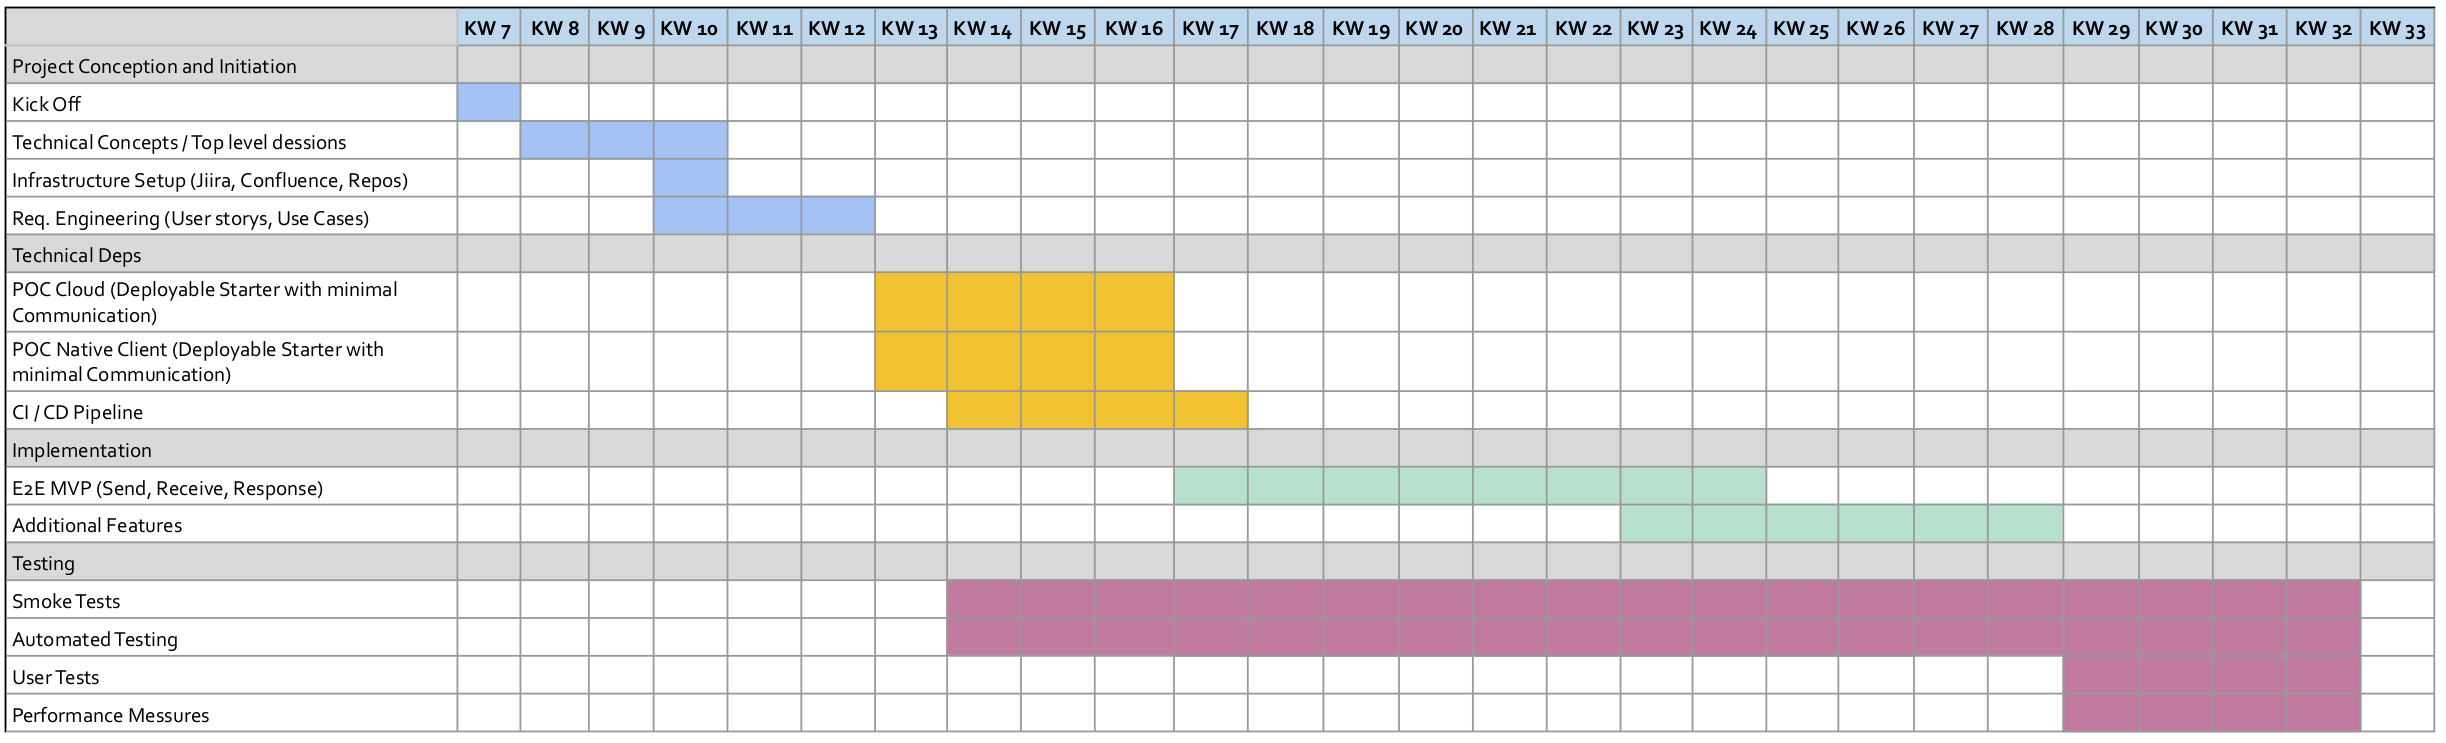
\includegraphics[width=\linewidth]{graphics/Projectplanning}\caption[Projektplan]{Projektplan}
\end{figure}

Das Projekt Cloudbasiertes Praxisrufsystem soll in vier Phasen umgesetzt werden.
Wobei sich diese Phasen teilweise überschneiden.

In der ersten Phase (KW7-KW13) wird die organisatorische Infrastruktur für das Projekt aufgebaut.
Es werden Grobkonzepte für das umzusetzende System erfasst.
Dazu werden Technologien evaluiert, die zur Umsetzung verwendet werden können und
die wichtigsten Ziele des Projektes als Milestones festgehalten.

In der zweiten Phase (KW13-KW17) wird ein Proof Of Concept erstellt.
Dieser soll die gültigkeit der Resultate aus Phase 1 verifizieren.
Wenn nötig werden hier Anpassungen an den gewählten Technologien und erstellten Grobkonzepten gemacht.
Die Architektur und das Konzept werden weiter verfeinert und erste Anforderungen werden konkretisiert.

In der dritten Phase (KW17-KW38) wird das Projekt umgesetzt.
Zur Umsetzung gehört dabei, laufend die als nächstes umzusetzenden Anforderungen im Detail zu definieren und die Konzepte dafür zu erweitern.

Die vierte Phase (KW14-KW32) läuft parallel zur Dritten und beschäftigt sich mit dem Testen des Systems.
Automatisierte Unit und Smoke Tests sollen während der ganzen Projektdauer für die entwickelten Komponenten gemacht werden.
Zum Ende des Projekts soll das System zudem mit dem Benutzer getestet werden und auf Performance geprüft werden.

\clearpage
\subsection{Milestones}

In der Anfangsphase des Projektes wurden folgende Milestones definiert:

\begin{table}[h]
    \centering
    \begin{tabular}{|l|p{15cm}|}
        \hline
        \textbf{Id} & \textbf{Beschreibung}                                                                                                                                                                                         \\
        \hline
        M01         & Proof Of Concept - Setup. Ein Mobile Client kann auf IOS installiert werden und mit einem Backendservice kommunizieren. \\
        \hline
        M02         & Proof Of Concept - Messaging. Ein Mobile Client kann Benachrichtigungen empfangen und Push-Benachrichtigungen anzeigen. \\
        \hline
        M03         & Versenden mit Registration. Mobile Clients können sich beim Praxisrufsystem registrieren und Benachrichtungen empfangen. Alle registrierten Clients erhalten alle Benachrichtigungen. \\
        \hline
        M04         & Benachrichtigungen konfigurierbar. Der Mobile Client lädt seine Konfiguration vom Backend und zeigt dynamisch konfigurierte Buttons an über die Benachrichtigungen versendet werden.\\
        \hline
        M05         & Setup Wizard für Konfiguration. Ein Administrator kann das System über eine Benutzeroberfläche konfigurieren.  \\
        \hline
        M06         & 1:N Versenden Konfigurierbar. Es kann konfiguriert werden, welcher Client sich für welche Benachrichtigungen interessiert. Alle Clients erhalten nur für sie relevante Benachrichtigungen.  \\
        \hline
        M07         & Voice to Speech. Empfangene Benachrichtigungen können dem Benutzer vorgelesen werden. \\
        \hline
        M08         & Raspberry Pi Anbindung. Benachrichtigungen können über ein Raspberry Pi mit angeschlossenem Button versendet werden. \\
        \hline
        M09         & Sprachkommunikation 1:1. Der Mobile Client unterstützt direkte Anrufe zwischen zwei Geräten. \\
        \hline
        M10         & Sprachkommunikation 1:n. Der Mobile Client unterstützt Gruppenanrufe mit mehreren Geräten gleichzeitig. \\
        \hline
    \end{tabular}\label{tab:milestones}
\end{table}
\clearpage



    \section{Anforderungen}\label{sec:anforderungen}

Die umzusetzenden Anforderungen wurden während des Projektes iterativ zusammen mit dem Kunden erarbeitet.
Dieses Kapitel zeigt den Stand der erarbeiteten Anforderungen bei Projektabschluss.
Alle Anforderungen wurden zuerst aus fachlicher Sicht mit User Stories festgehalten.
Jede User Story beschreibt ein konkretes Bedürfnis der Benutzer.
Die erfassten User Stories werden in drei Bereiche unterteilt.
Im ersten Bereich werden Bedürfnisse von Praxismitarbeitenden festgehalten.
Praxismitarbeitende verwendet die mobile Applikation von Praxisruf, um Benachrichtigungen zu versenden und empfangen.
Im zweiten Bereich werden die Bedürfnisse von Praxisveranwotrlichen beschrieben.
Diese Benutzergruppe ist dafür verantwortlich Praxisruf für Praxismitarbeitende zu konfigurieren.
In einem dritten Bereich werden User Stories aus Sicht des Kunden festhalten, welche Rahmenbedingungen und Bedürfnisse des Auftraggebers festhalten.
Aufgrund der User Stories werden Features definiert, welche konkrete testbare Szenarien und die erwarteten Ergebnisse definieren.\footnote{Siehe Anhang E - Features und Testszenarien}

\subsubsection*{Praxismitarbeitende}

\begin{table}[h]
    \centering
    \begin{tabular}{|l|p{13cm}|c|}
        \hline
        \textbf{Id} & \textbf{Anforderung}                                                                                                                                                                                         & \textbf{Feature} \\
        \hline
        U01         & Als Praxismitarbeiter/-in möchte ich Benachrichtigungen versenden können, damit ich andere Mitarbeitende über Probleme und Anfragen informieren kann. & F01 \\
        \hline
        U02         & Als Praxismitarbeiter/-in möchte ich Benachrichtigungen empfangen können, damit ich auf Probleme und Anfragen anderer Mitarbeitenden reagieren kann. & F02 \\
        \hline
        U03         & Als Praxismitarbeiter/-in möchte ich nur Benachrichtigungen sehen, die für mich relevant sind, damit ich meine Arbeit effizient gestalten kann. & F02 \\
        \hline
        U04         & Als Praxismitarbeiter/-in möchte ich über empfangene Benachrichtigungen aufmerksam gemacht werden, damit ich keine Benachrichtigungen verpasse. & F04 \\
        \hline
        U05         & Als Praxismitarbeiter/-in möchte ich sehen welche Benachrichtigungen ich verpasst habe, damit ich auf verpasste Benachrichtigungen reagieren kann. & F04 \\
        \hline
        U06         & Als Praxismitarbeiter/-in möchte ich eine Rückmeldung erhalten, wenn eine Benachrichtigung nicht versendet werden kann, damit Benachrichtigungen nicht verloren gehen. & F03 \\
        \hline
        U07         & Als Praxismitarbeiter/-in möchte ich auswählen können an welchem Gerät ich das Praxisrufsystem verwende und die dafür erstellte Konfiguration erhalten, damit das Praxisrufsystem optimal verwendet werden kann. & F05 \\
        \hline
        U08          & Als Praxismitarbeiter/-in möchte ich einen physischen Knopf am Behandlungsstuhl haben damit ich notifikationen darüber versenden kann. & F07 \\
        \hline
        U09          & Als Praxismitarbeiter/-in möchte ich, dass mir Benachrichtigungen vorgelesen werden, damit ich informiert werde, ohne meine Arbeit unterbrechen zu müssen. & F08 \\
        \hline
        U10         & Als Praxismitarbeiter/-in möchte ich einen anderen Client Unterhaltungen führen können damit Fragen direkt geklärt werden können. & F09 \\
        \hline
        U11         & Als Praxismitarbeiter/-in möchte ich Unterhaltungen mit mehreren anderen Clients gleichzeitig führen können damit komplexe Fragen direkt geklärt werden können. & F10 \\
        \hline
    \end{tabular}\label{tab:userstories1}
\end{table}

\clearpage

\subsubsection*{Praxisverantwortliche}

\begin{table}[h]
    \centering
    \begin{tabular}{|l|p{13cm}|c|}
        \hline
        \textbf{Id} & \textbf{Anforderung}                                                                                                                                                                               & \textbf{Features} \\
        \hline
        U12         & Als Praxisverantwortliche/-r möchte ich mehrere Geräte verwalten können, damit das Praxisrufsystem in mehreren Zimmern gleichzeitig genutzt werden kann. & F06 \\
        \hline
        U13         & Als Praxisverantwortliche/-r möchte ich definieren können, welches Gerät welche Anfragen versenden kann, damit jedes Gerät Verwendungsort optimiert ist. & F06 \\
        \hline
        U14         & Als Praxisverantwortliche/-r möchte ich die Konfiguration des Praxisrufsystems zentral verwalten können, damit das Praxisrufsystem für die Anwender optimiert werden kann. & F06 \\
        \hline
        U15         & Als Praxisverantwortliche/-r möchte ich definieren können, welche Geräte mit welchen anderen Geräten telefonieren können damit alle Mitarbeitenden die Gegensprechanlage nutzen können. & F06 \\
        \hline
        U16         & Als Praxisverantwortliche/-r möchte ich definieren können, welche Benachrichtigung über einen physischen Knopf am Behandlungsstuhl versendet wird damit der Knopf für die Mitarbeitenden optimiert ist. & F06 \\
        \hline
    \end{tabular}\label{tab:userstories2}
\end{table}

\subsubsection*{Auftraggeber}\label{subsec:auftraggeber}

\begin{table}[h]
    \centering
    \begin{tabular}{|l|p{13cm}|c|}
        \hline
        \textbf{Id} & \textbf{Anforderung}                                                                                                                                                                          & \textbf{Features} \\
        \hline
        T01         & Als Auftraggeber möchte ich, dass das Praxisrufsystem über IPads bedient werden kann, damit ich von bestehender Infrastruktur profitieren kann. & n/A \\
        \hline
        T02         & Als Auftraggeber möchte ich, dass das Praxisrufsystem über Android Tablets bedient werden kann, damit es in Zukunft für eine weitere Zielgruppe verwendet werden kann. & n/A \\
        \hline
        T03         & Als Auftraggeber möchte ich, dass die Codebasis für das Praxisrufsystem für Android und IOS verwendet werden kann, damit ich die Weiterentwicklung optimieren kann. & n/A \\
        \hline
        T04         & Als Auftraggeber möchte ich, dass wo möglich der Betrieb von Serverseitigen Dienstleistungen über AWS betrieben wird, damit ich von bestehender Infrastruktur und Erfahrung profitieren kann. & n/A               \\
        \hline
    \end{tabular}\label{tab:userstories3}
\end{table}

\clearpage


    \section{Evaluation Technologien}\label{sec:evaluation-technologien}

\subsection{Mobile Client Evaluation}\label{subsec:mobile-client-eval}



\url{https://kotlinlang.org/lp/mobile/}
	

    +Jet Brains Infrastructure 
    +We like Kotlin 

    -IoS Env. Needed to develop for Apple 
    -Still has to develop separate API und UI Modules for Platforms 

\url{https://web.dev/progressive-web-apps/ }
	
    +No need of Native Codebase
    +Perfect for Android 
    -Eventually drawbacks because no entire API Access 
    -PWAs on IOS suck

\url{https://cordova.apache.org/} 
	

    + Popular Framework 
    + Tons of plugins to access apis 

    -Still need to have a Mac for IoS development  
    -Not a truly native app -> API Issues
 

\url{https://nativescript.org/ }

    +Provides a Workaround for nasty X-tools 
    +Claims to be truly Native 
    -Do we really trust it? (sorta new and passion project of a few people) 

 
 \url{https://flutter.dev}

    -Why do you hate me?


"Simply Write Everything twice"

    +Would definitely work

    -Do most things twice
    -We don't have time for that
    -Kunde wünscht ausdrücklich nur eine Codebasis für beide Clients.

\url{https://stackshare.io/stackups/apache-cordova-vs-nativescript}

\url{https://nativescript.org/blog/build-nativescript-apps-remotely-from-windows-or-linux/ }

\subsection{Messaging Service}\label{subsec:messaging-eval}

Für das Praxisrufsystem wird ein Dienst benötigt mit dem Benachrichtigungen an eine Mobile Applikation gesendet werden können.
Als Reaktion auf eine empfangene Benachrichtigung muss es möglich sein, Push-Benachrichtigungen auf dem Gerät anzuzeigen.
Die Technologie die dazu verwendet wird, muss dabei mit der für den Mobile Client gewählten Technologie kompatibel sein.
Für den Mobile Client wurde das Native Script Framework ausgewählt.
Damit sind Push-Benachrichtigungen auf iOS und Android möglich.
Push-Benachrichtigungen auf iOS sind dabei nur über die Anbindung von Firebase Messaging (FCM) möglich.\cite{nativescript-push}

Um Mobile CLients über Benachrichtigungen zu informieren ist es möglich mit EventSources\cite{event-source} Anfragen von der Serverseite an einen Client zu senden.
Dies hat allerdings den Nachteil, dass eine Konstante HTTP Verbindung zwischen Client und Server bestehen muss.

Weiter besteht die Möglichkeit, über einen Messaging Broker Benachrichtigungen an den Mobile Client zu senden.
Hier besteht allerdings dasselbe Problem.
Damit Benachrichtigungen auf der Client Seite Empfangen werden können, muss eine Verbindung zum Messaging Broker bestehen. //TODO @Kevin: Any Idea how to cite this? I know it's true, but citable source would be nice.

Sowohl die Option "EventSources" als auch die Option "Message Broker" haben zudem die Einschränkung, dass sie es nicht ermöglichen Push-Benachrichtigungen anzuzeigen.
Um dies auf iOS mit Nativescript zu ermöglichen müsste zusätzlich ein Firebase Messaging Service angebunden werden.

FCM ermöglicht es dabei selbst von einem Server Umfeld Benachrichtigungen an Endgeräte zu versenden.\cite{fcm-java}
Firebase Messaging unterstützt damit die Anforderungen, von einem Cloud Server Benachrichtigungen an einen Mobile Client zu senden und Push-Benachrichtigungen auf dem Gerät anzuzeigen.
In der Folge wird für das Praxisrufsystem auschliessliche Firebase Messaging als Messaging Service verwendet.

\subsection{Cloud Service}\label{subsec:cloud-service2}

Cloud Services die für das Praxisrufsystem nötig sind, werden mit Java und Spring Boot umgesetzt.
Spring Boot vereinfacht Grundlagenarbeit die zum Aufsetzen eines Backendservices nötig sind und bietet
gleichzeitig die Werkzeuge die nötig sind um sichere, skalierbare Microservices zu implementieren.\cite{why-spring}
Spring und Java sind zudem Technologien, mit welchen alle Projektteilnehmer bereits Erfahrung gesammelt haben.
Diese für die Umsetzung in diesem Projekt zu verwenden, ermöglicht es die nötigen Services noch effizienter umzusetzen
und den Fokus auf das Technische Konzept sowie die Anforderungsanalyse zu legen.

In der Anforderung T04\footnote{Siehe Kapitel 3} ist vorgegeben, dass der Betrieb aller Cloud- und Web-Applikationen mit Amazon Webservices erfolgen muss.
Mit Elastic Beanstalk von AWS ist die der Betrieb von Java Applikationen auf AWS möglich.\cite{aws-spring-java}



    \section{Konzept}\label{sec:konzept}

\subsection{Systemarchitektur}\label{subsec:systemarchitektur}
\subsubsection*{Abgrenzung}

Dieses Kapitel gibt einen Übersicht über die Systemarchitektur als ganzes. Die Architektur beschränkt sich dabei auf die
Anforderungen die innerhalb des Projektrahmens umgesetzt wurden. Komponenten für Teile die Out Of Scope gefallen sind,
werden hier nicht behandelt.

\subsubsection*{Übersicht}

Das cloudbasierte Praxisrufsystem wird in vier Komponenten unterteilt.
Im Zentrum steht eine cloudbasierte Applikation (Cloud Service) welche es ermöglicht Konfigurationen persistent zu verwalten und das Versenden von Benachrichtigungen anhand dieser Konfigurationen koordiniert.
Der Cloud Service benutzt einen externen Messaging Service zum Versenden von Benachrichtigungen. Dabei ist der Messaging Service lediglich für die Zustellung von Benachrichtigungen verantwortlich.
Zur Verwaltung der Konfigurationen wird ein Web Frontend (Admin UI) erstellt. Dieses bietet einem Administrator die Möglichkeit Konfigurationen aus dem Cloud Service zu lesen, erstellen, bearbeiten und löschen.
Die Konfigurationen die über Admin UI und Cloud Service erstellt wurden, werden schliesslich von einem Mobile Client. Mit dem Mobile Client kann der Benutzer Benachrichtigungen an andere Mobile Clients senden.
Welche Benachrichtigungen ein Mobile Client senden kann und an wen diese Benachrichtungen zugstellt werden, wird anhand der Konfiguration aus dem Cloud Service bestimmt.

\begin{figure}[h]
    \centering
    \begin{minipage}[b]{1.0\textwidth}
        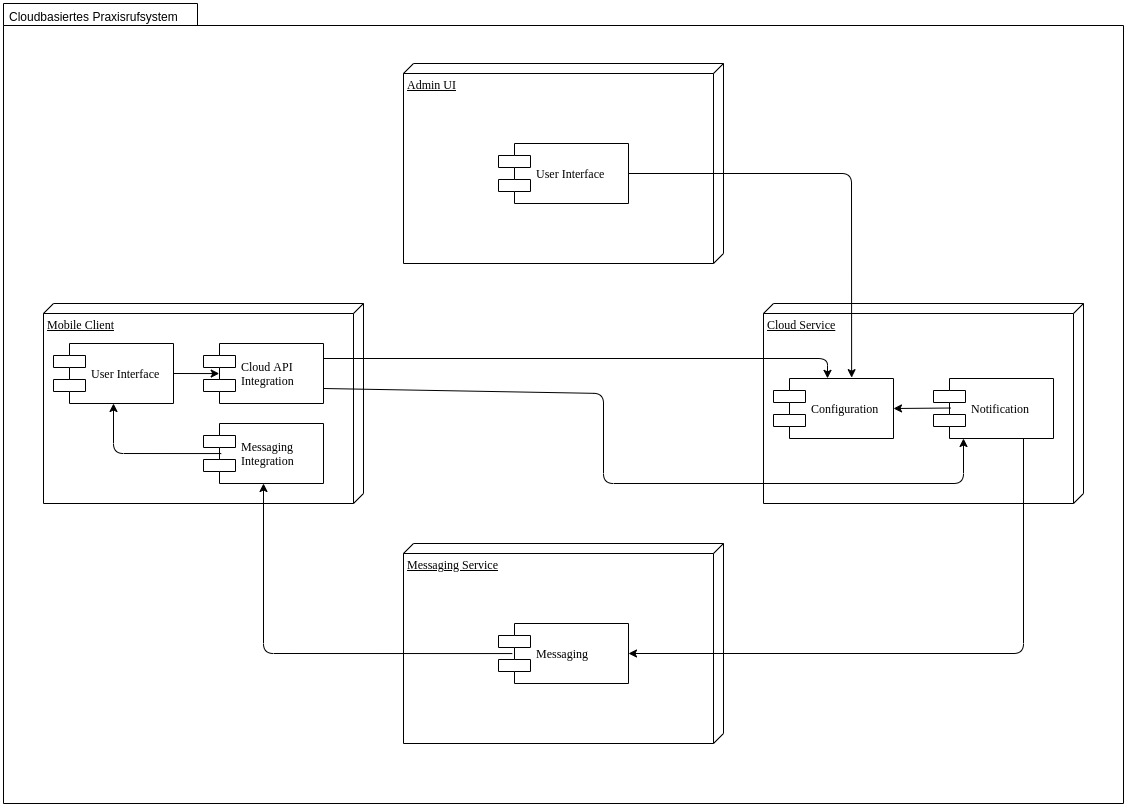
\includegraphics[width=\textwidth]{graphics/Component_System}
        \caption{System}
    \end{minipage}
\end{figure}

\clearpage

Die Anforderungen U12 setzt voraus, dass die Kommunikation im Praxisrufsystem
zwischen mehreren Geräten erfolgen kann.

Die Anforderungen U06, U07 und U13 setzten voraus, dass die es eine zentrale Stelle gibt
die Konfigurationen zur Verfügung stellt und das Versenden von Notifikationen koordiniert.


\subsubsection*{Mobile Client}

\begin{itemize}
    \item Der Mobile Client implementiert die Anbindung an den Messaging Service.
    \item Als Reaktion auf eine Notification wird eine Rückmeldung im UI angezeigt.
    \item Als Reaktion auf eine Notification wird eine OS Push Notifikation gesendet.
    Das UI bietet einen Button der eine Anfrage an die REST Schnittstelle im Cloud Service sendet.
\end{itemize}


\subsubsection*{Cloud Service}

\begin{itemize}
    \item Responsibilities (Notification and Configuration)
    \item Microservice Granularity
\end{itemize}


\subsubsection*{Messaging Service}

\begin{itemize}
    \item Dies wird ein externer Service den wir in die Applikationen einbinden. Standard hierfür ist Firebase Notifications.
    \item Der Messaging Service nimmt Notifikationen vom Cloud Service entgegen und gibt diese an den Mobile Client wieder.
    \item Dafür müssen auf beiden Seiten Komponenten eingebaut werden, die mit dem Messaging Service kommunizieren.
\end{itemize}

\clearpage

\subsubsection{Mobile Client}\label{subsec:mobile-client-realisation}

Dieses Kapitel zeigt die umgesetzten Ansichten des Mobile Clients.
Weitere Informationen zur Bedienung des Mobile Clients sind dem Benutzerhandbuch zu entnehmen\footnote{Siehe Anhang C}.

\subsubsection*{Anmeldung und Konfiguration}

Wird die Mobile Client Applikation zu ersten Mal geöffnet, muss die korrekte Konfiguration geladen werden.
So können Buttons für die benötigten Benachrichtigungen angezeigt und relevante Benachrichtigungen empfangen werden.
In einem ersten Schritt wird dem Benutzer deshalb eine einfache Login-Maske angezeigt.
Darin kann sich der Benutzer mit Benutzername und Passwort anmelden.
War die Anmeldung erfolgreich, werden alle Konfigurationen geladen, die dem Benutzer zur Verfügung stehen.
Die verfügbaren Konfigurationen werden dem Benutzer in einer Liste angezeigt und er wird aufgefordert, die gewünschte Konfiguration auszuwählen.
Nachdem die Auswahl erfolgt ist, wird der Benutzer zur Startseite weitergeleitet.

\begin{figure}[h]
    \centering
    \begin{minipage}[b]{0.4\textwidth}
        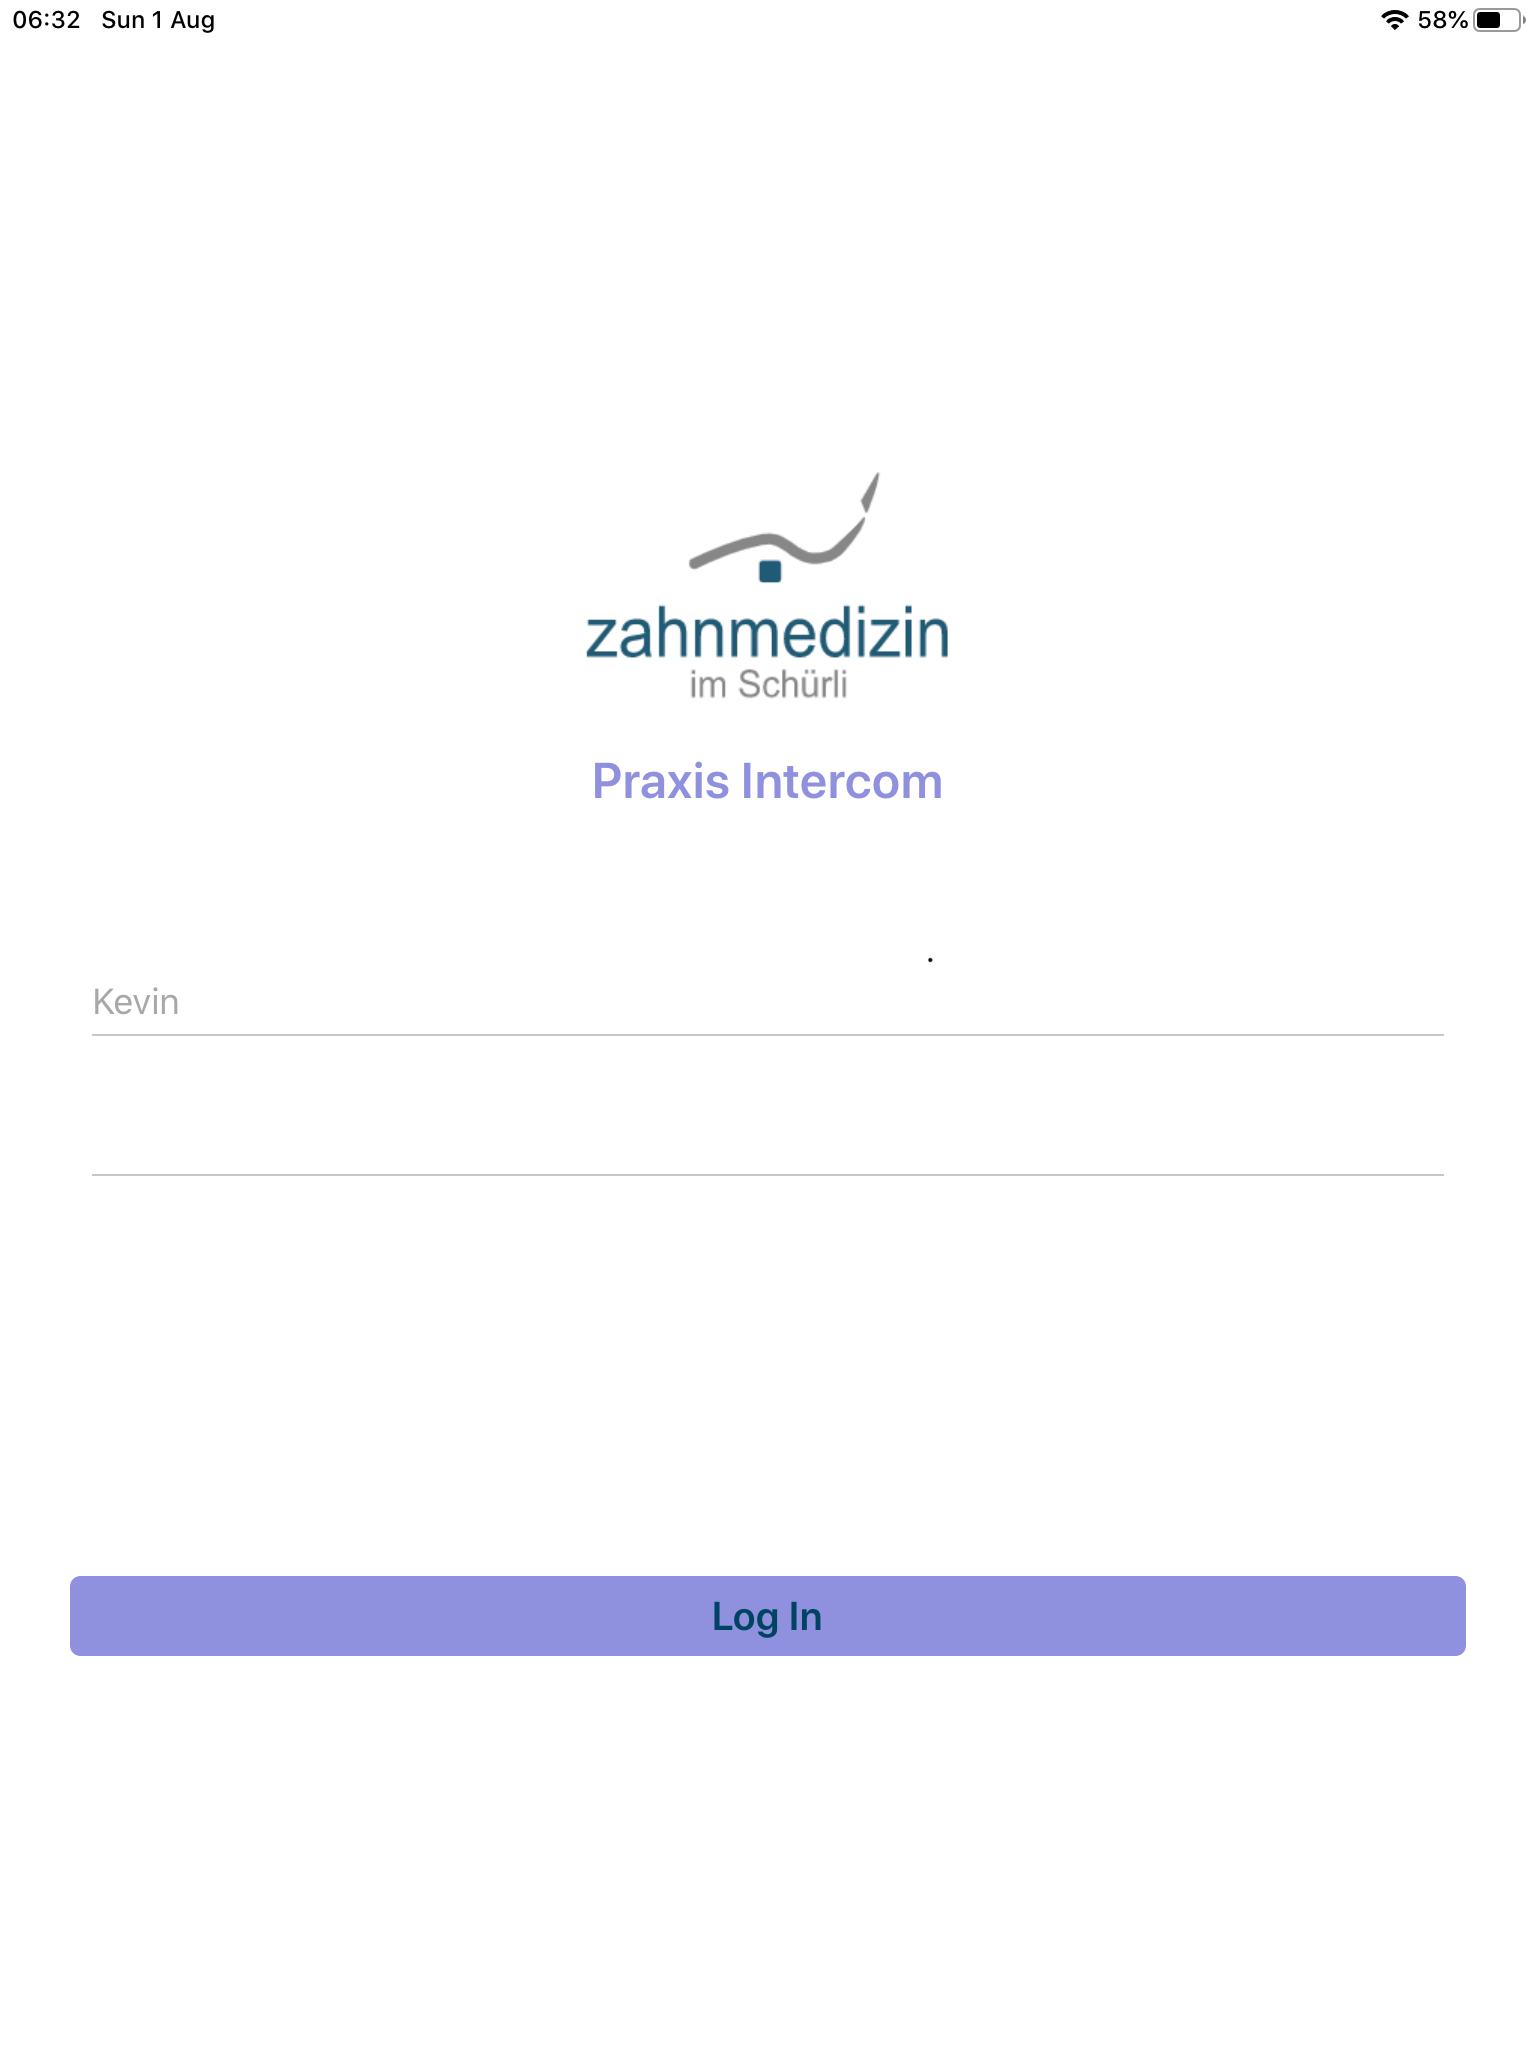
\includegraphics[width=\textwidth]{graphics/screenshots/mobileclient/screenshots-login}
        \caption{Login}
    \end{minipage}
    \hfill
    \begin{minipage}[b]{0.4\textwidth}
        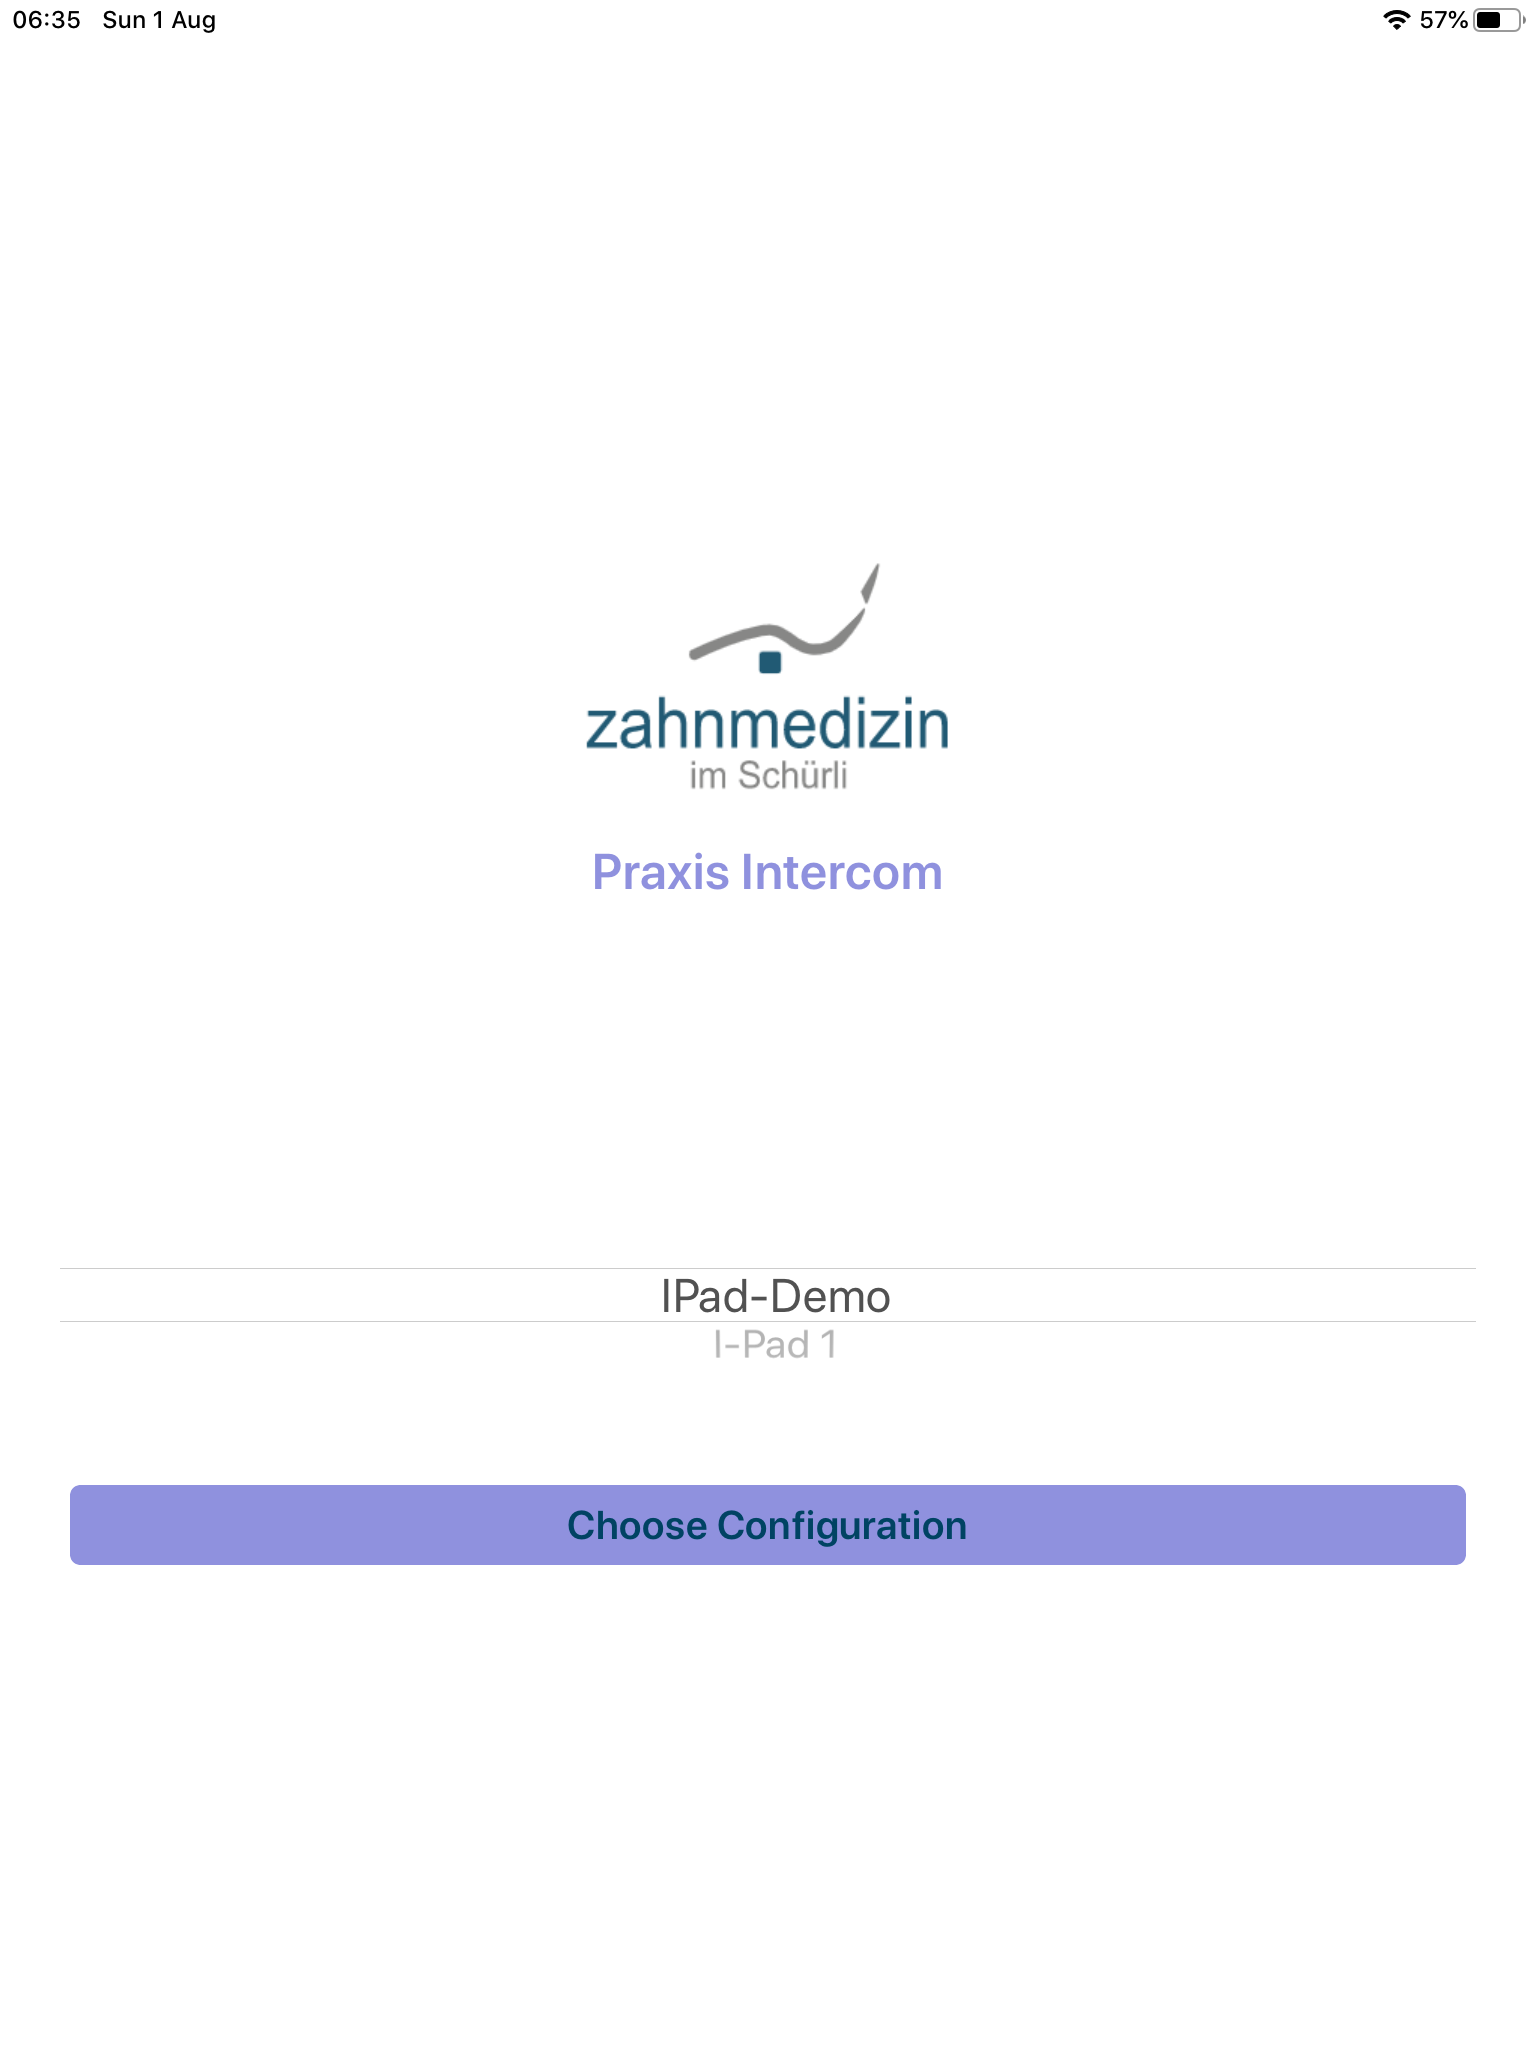
\includegraphics[width=\textwidth]{graphics/screenshots/mobileclient/screenshot-select-config}
        \caption{Konfiguration}
    \end{minipage}
    \label{fig:MobileClient-Screens1}
\end{figure}

\clearpage

\subsubsection*{Benachrichtigungen versenden}

Im Tab Home der Startseite werden Buttons angezeigt, um Benachrichtigungen zu versenden.
Die Buttons werden dynamisch aus der geladenen Konfiguration generiert.
Dabei gibt die Konfiguration den Text vor, der auf dem Button angezeigt wird.
Der Inhalt der Benachrichtigung, die der Button auslöst, ist in der Konfiguration im Cloud Service hinterlegt.

Tippt der Benutzer auf einen der Buttons, wird die entsprechende Benachrichtigung versendet.
Die Vermittlung, an die relevanten Empfänger übernimmt dabei der Cloud Service.
Dieser entscheidet anhand der vorhandenen Konfiguration, welchen Clients die Benachrichtigung zugestellt wird.
Schlägt das Versenden der Benachrichtigung an mindestens einen Empfänger fehl, wird dies dem Benutzer angezeigt.
Der Benutzer hat dann die Möglichkeit, das Versenden an diese Empfänger wiederholen.

\begin{figure}[h]
    \centering
    \begin{minipage}[b]{0.4\textwidth}
        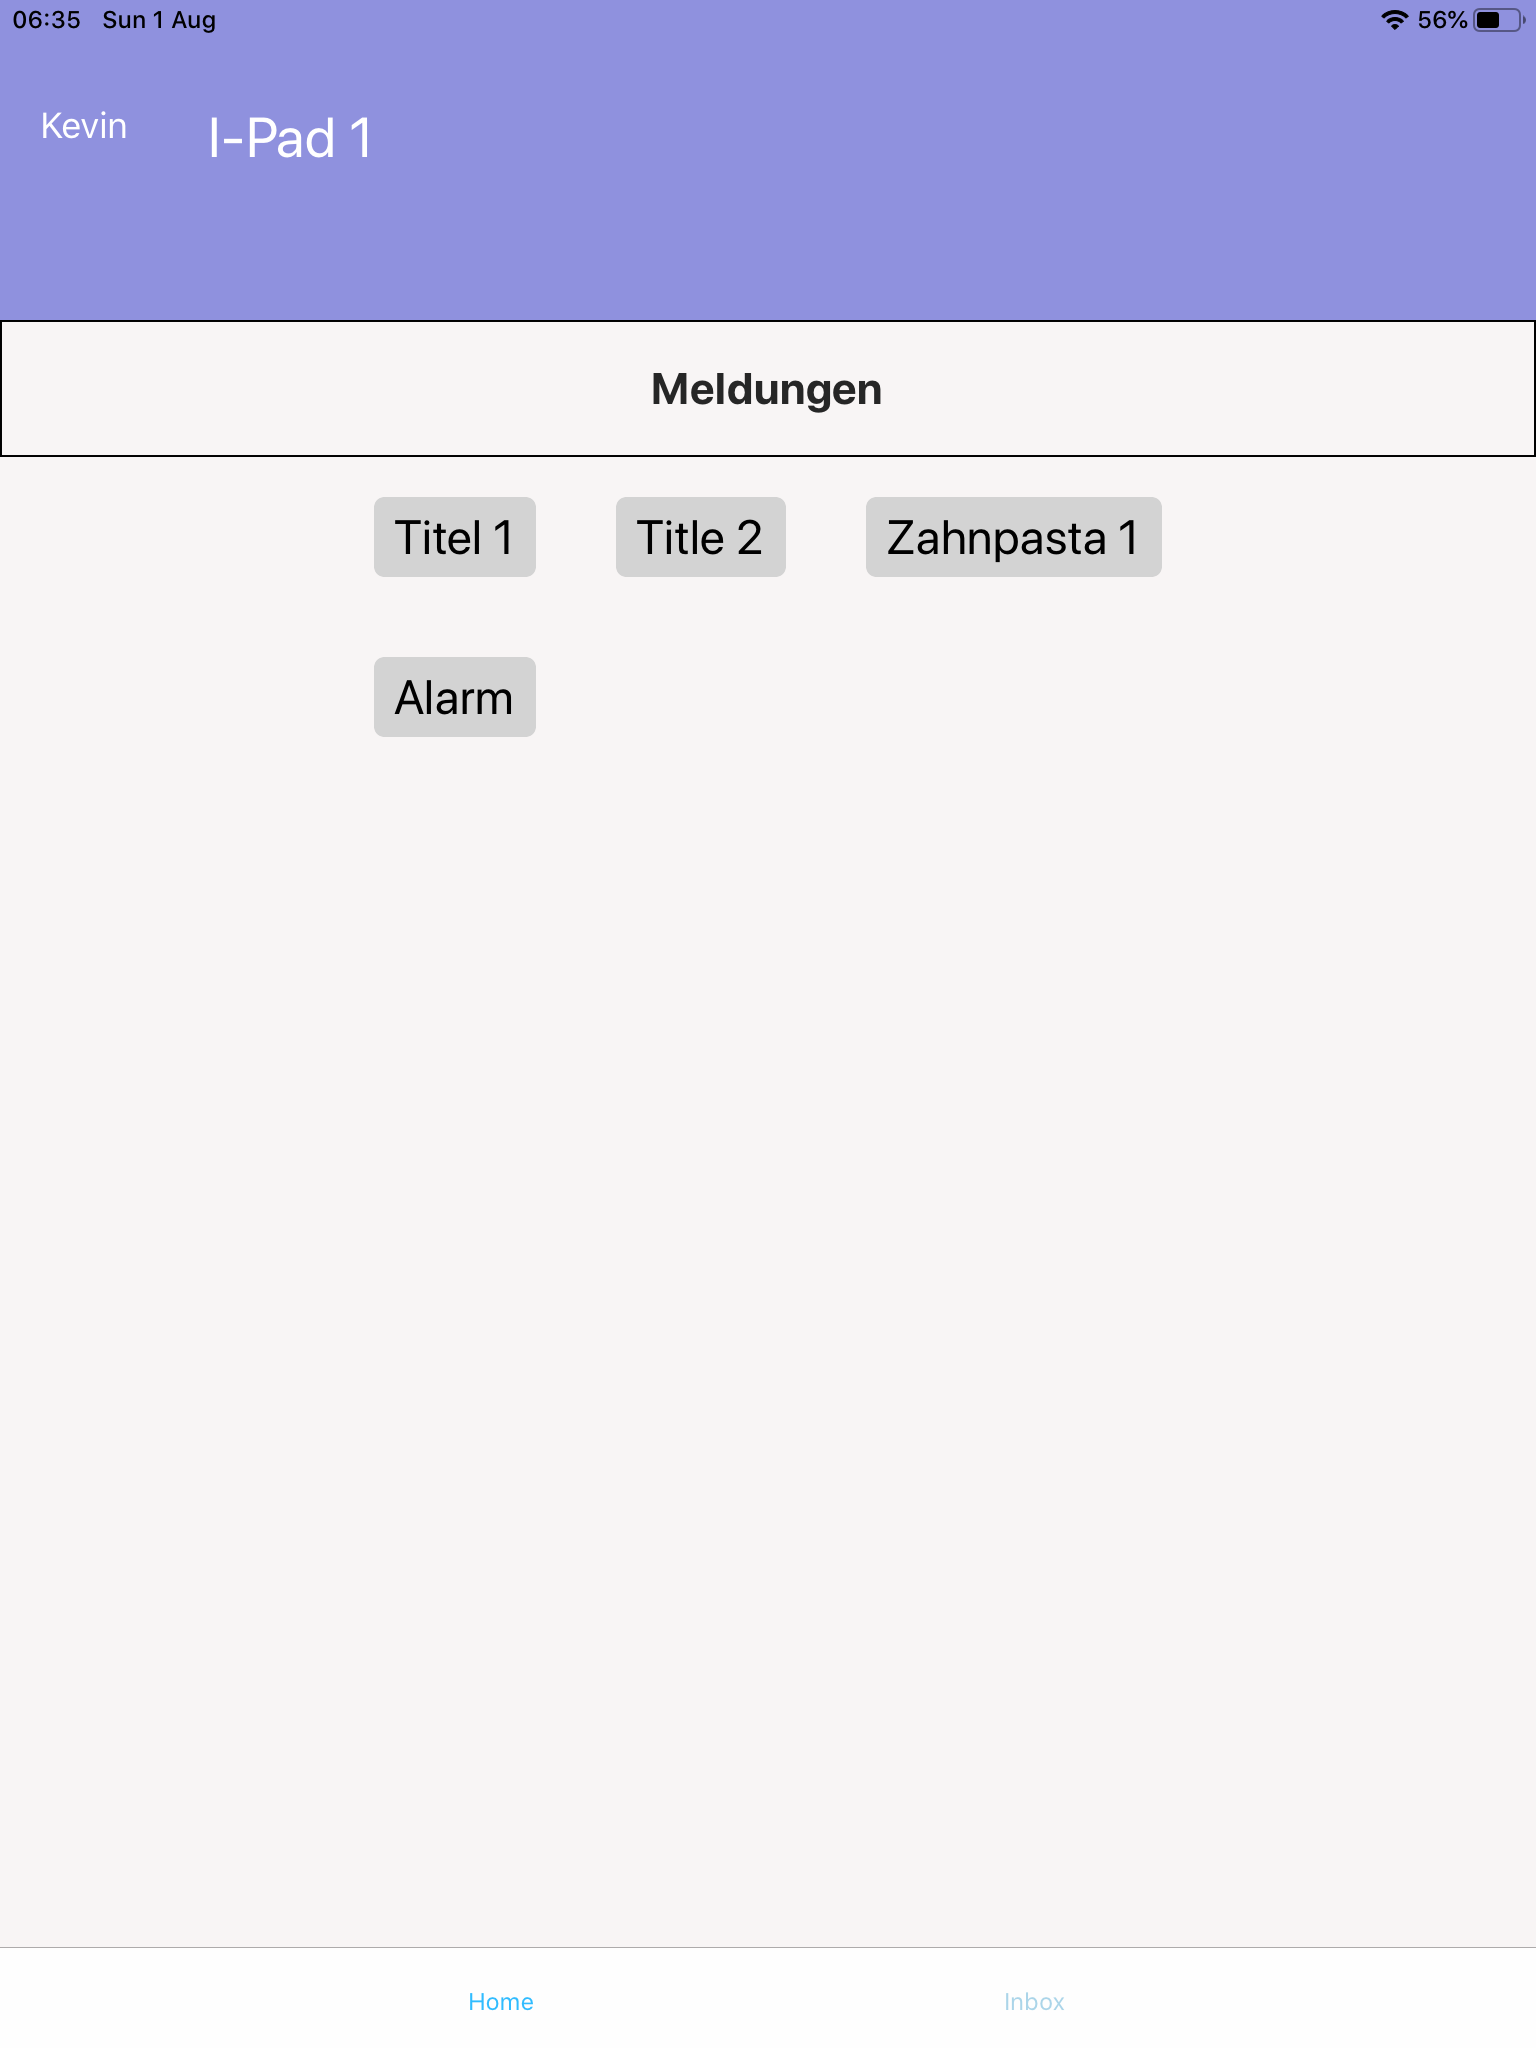
\includegraphics[width=\textwidth]{graphics/screenshots/mobileclient/screenshot-homescreen}
        \caption{Home}
    \end{minipage}
    \hfill
    \begin{minipage}[b]{0.4\textwidth}
        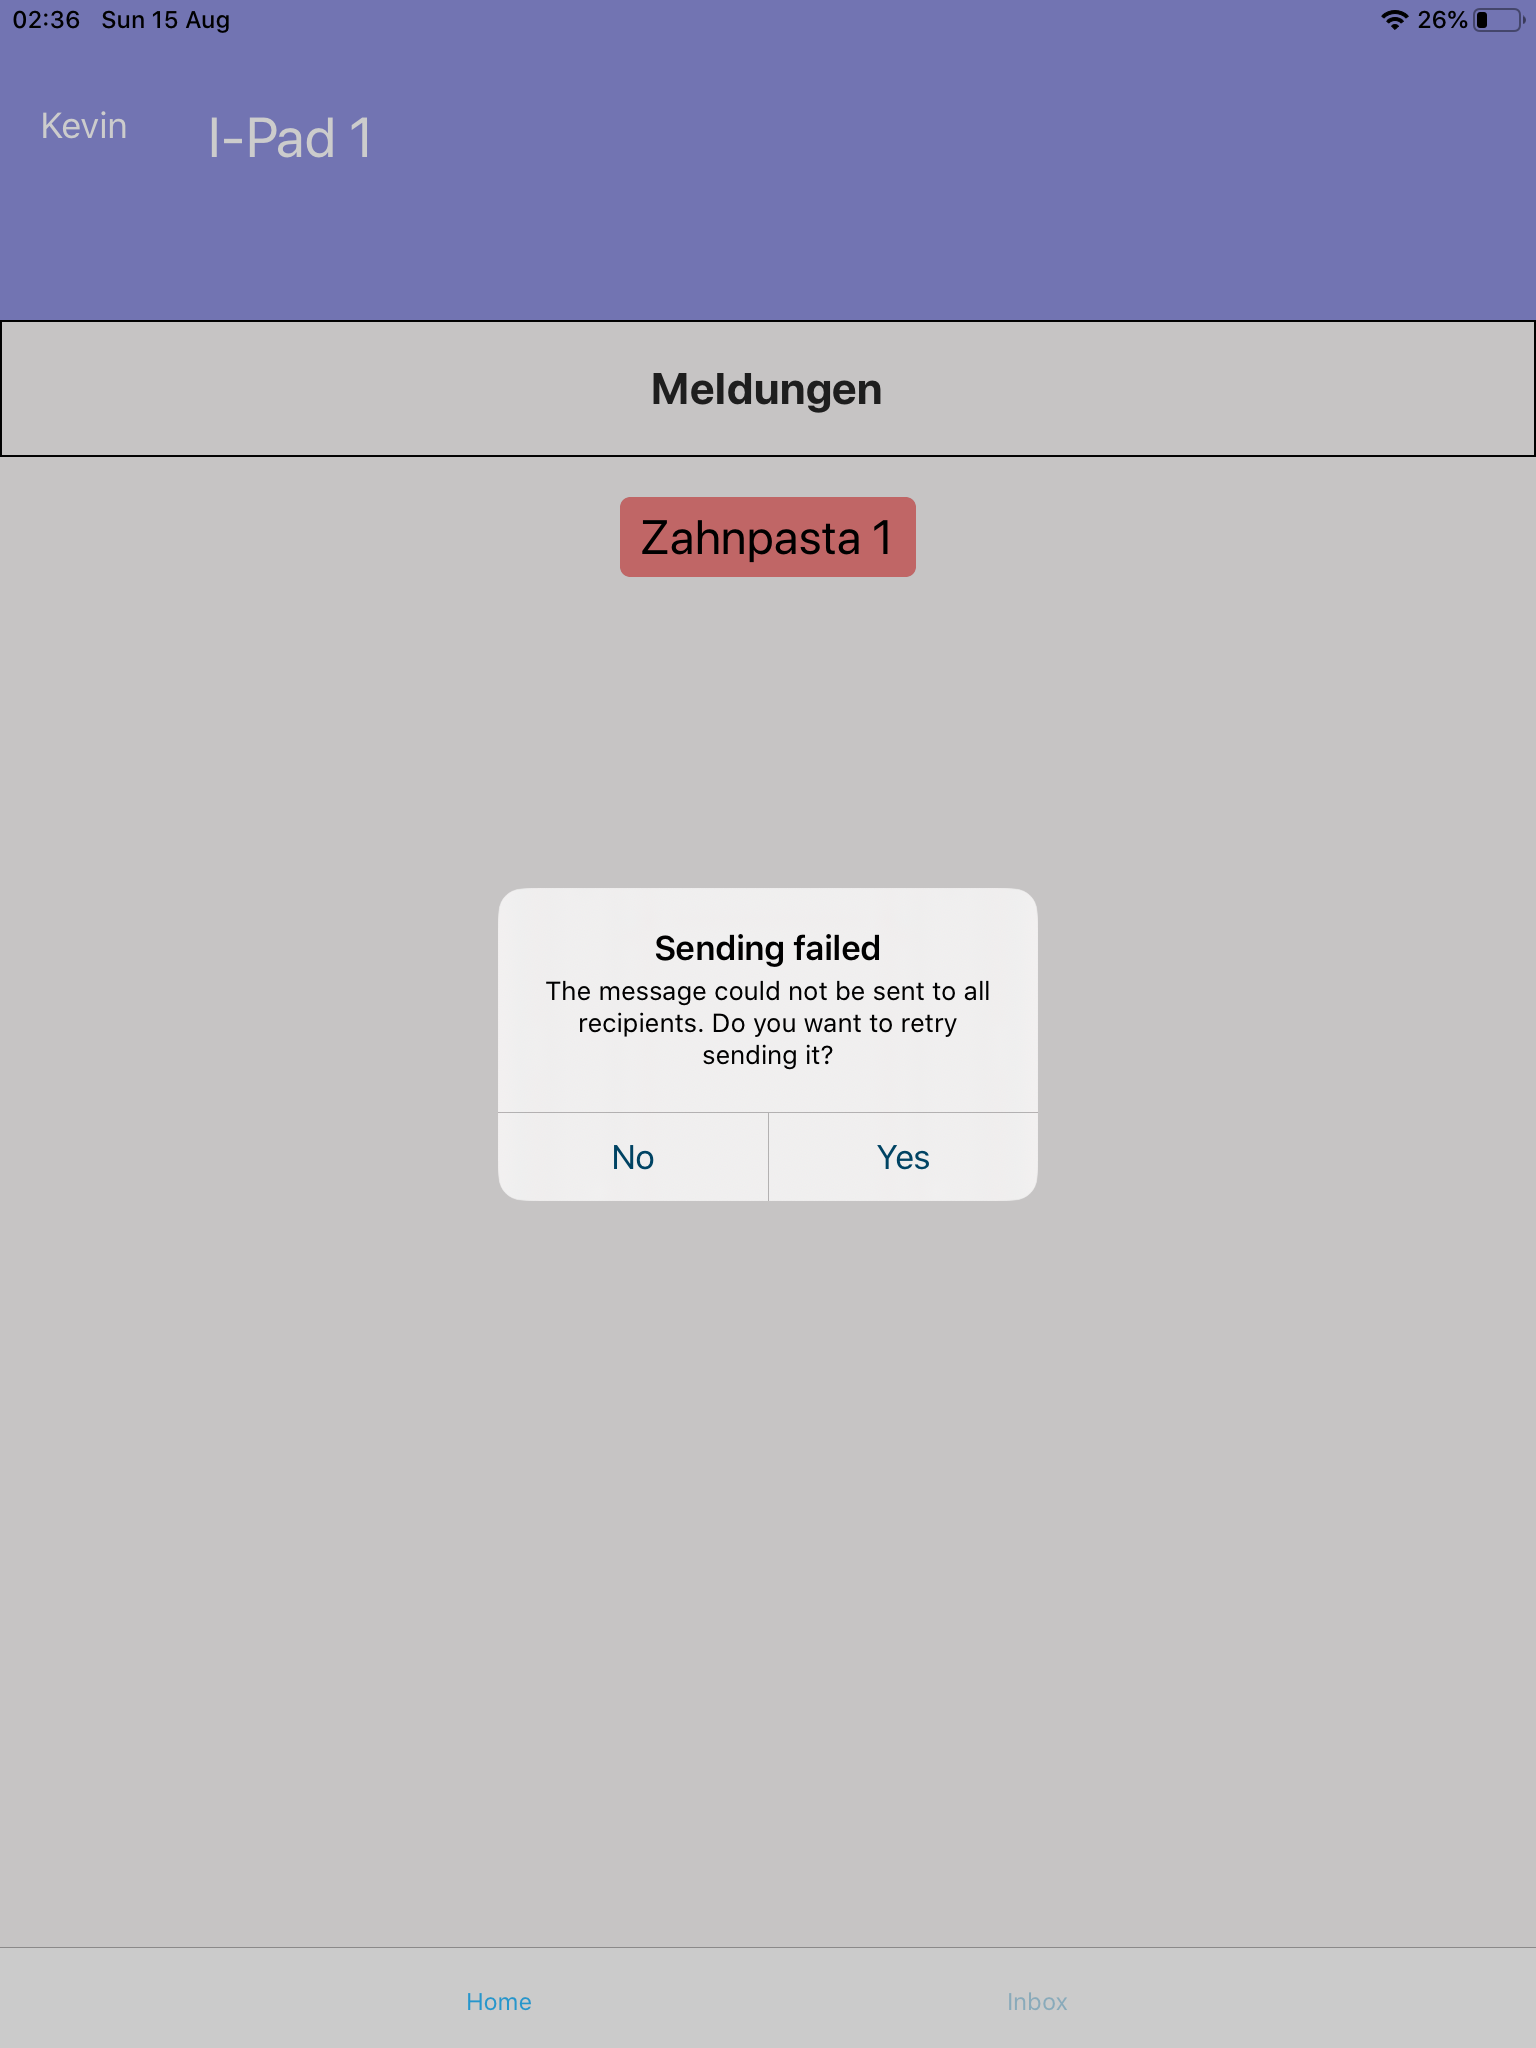
\includegraphics[width=\textwidth]{graphics/screenshots/mobileclient/screenshot-retry}
        \caption{Retry}
    \end{minipage}
    \label{fig:MobileClient-Screens2}
\end{figure}

\clearpage

\subsubsection*{Benachrichtigungen empfangen}

Wurde eine Benachrichtigung empfangen, ertönt ein Audio Signal und die Benachrichtigung ist im Tab Inbox auf der Startseite ersichtlich.
Durch Klick auf einen der Einträge in der Liste, kann der Benutzer die empfangene Benachrichtigung quittieren.
Wenn die Inbox Benachrichtigungen enthält, die nicht quittiert wurden, wiederholt der Client im Abstand von 30 Sekunden.
Die Quittierung von Benachrichtigungen erfolgt nur lokal auf dem Gerät.
Der Versender wird nicht über die Quittierung benachrichtigt.
Wurde eine Benachrichtigung im Hintergrund empfangen, wird diese als Push-Benachrichtigung auf dem Gerät angezeigt.
Auch wenn die Benachrichtigung im Hintergrund empfangen wurde, wird diese in der Inbox angezeigt.

\begin{figure}[h]
    \centering
    \begin{minipage}[b]{0.4\textwidth}
        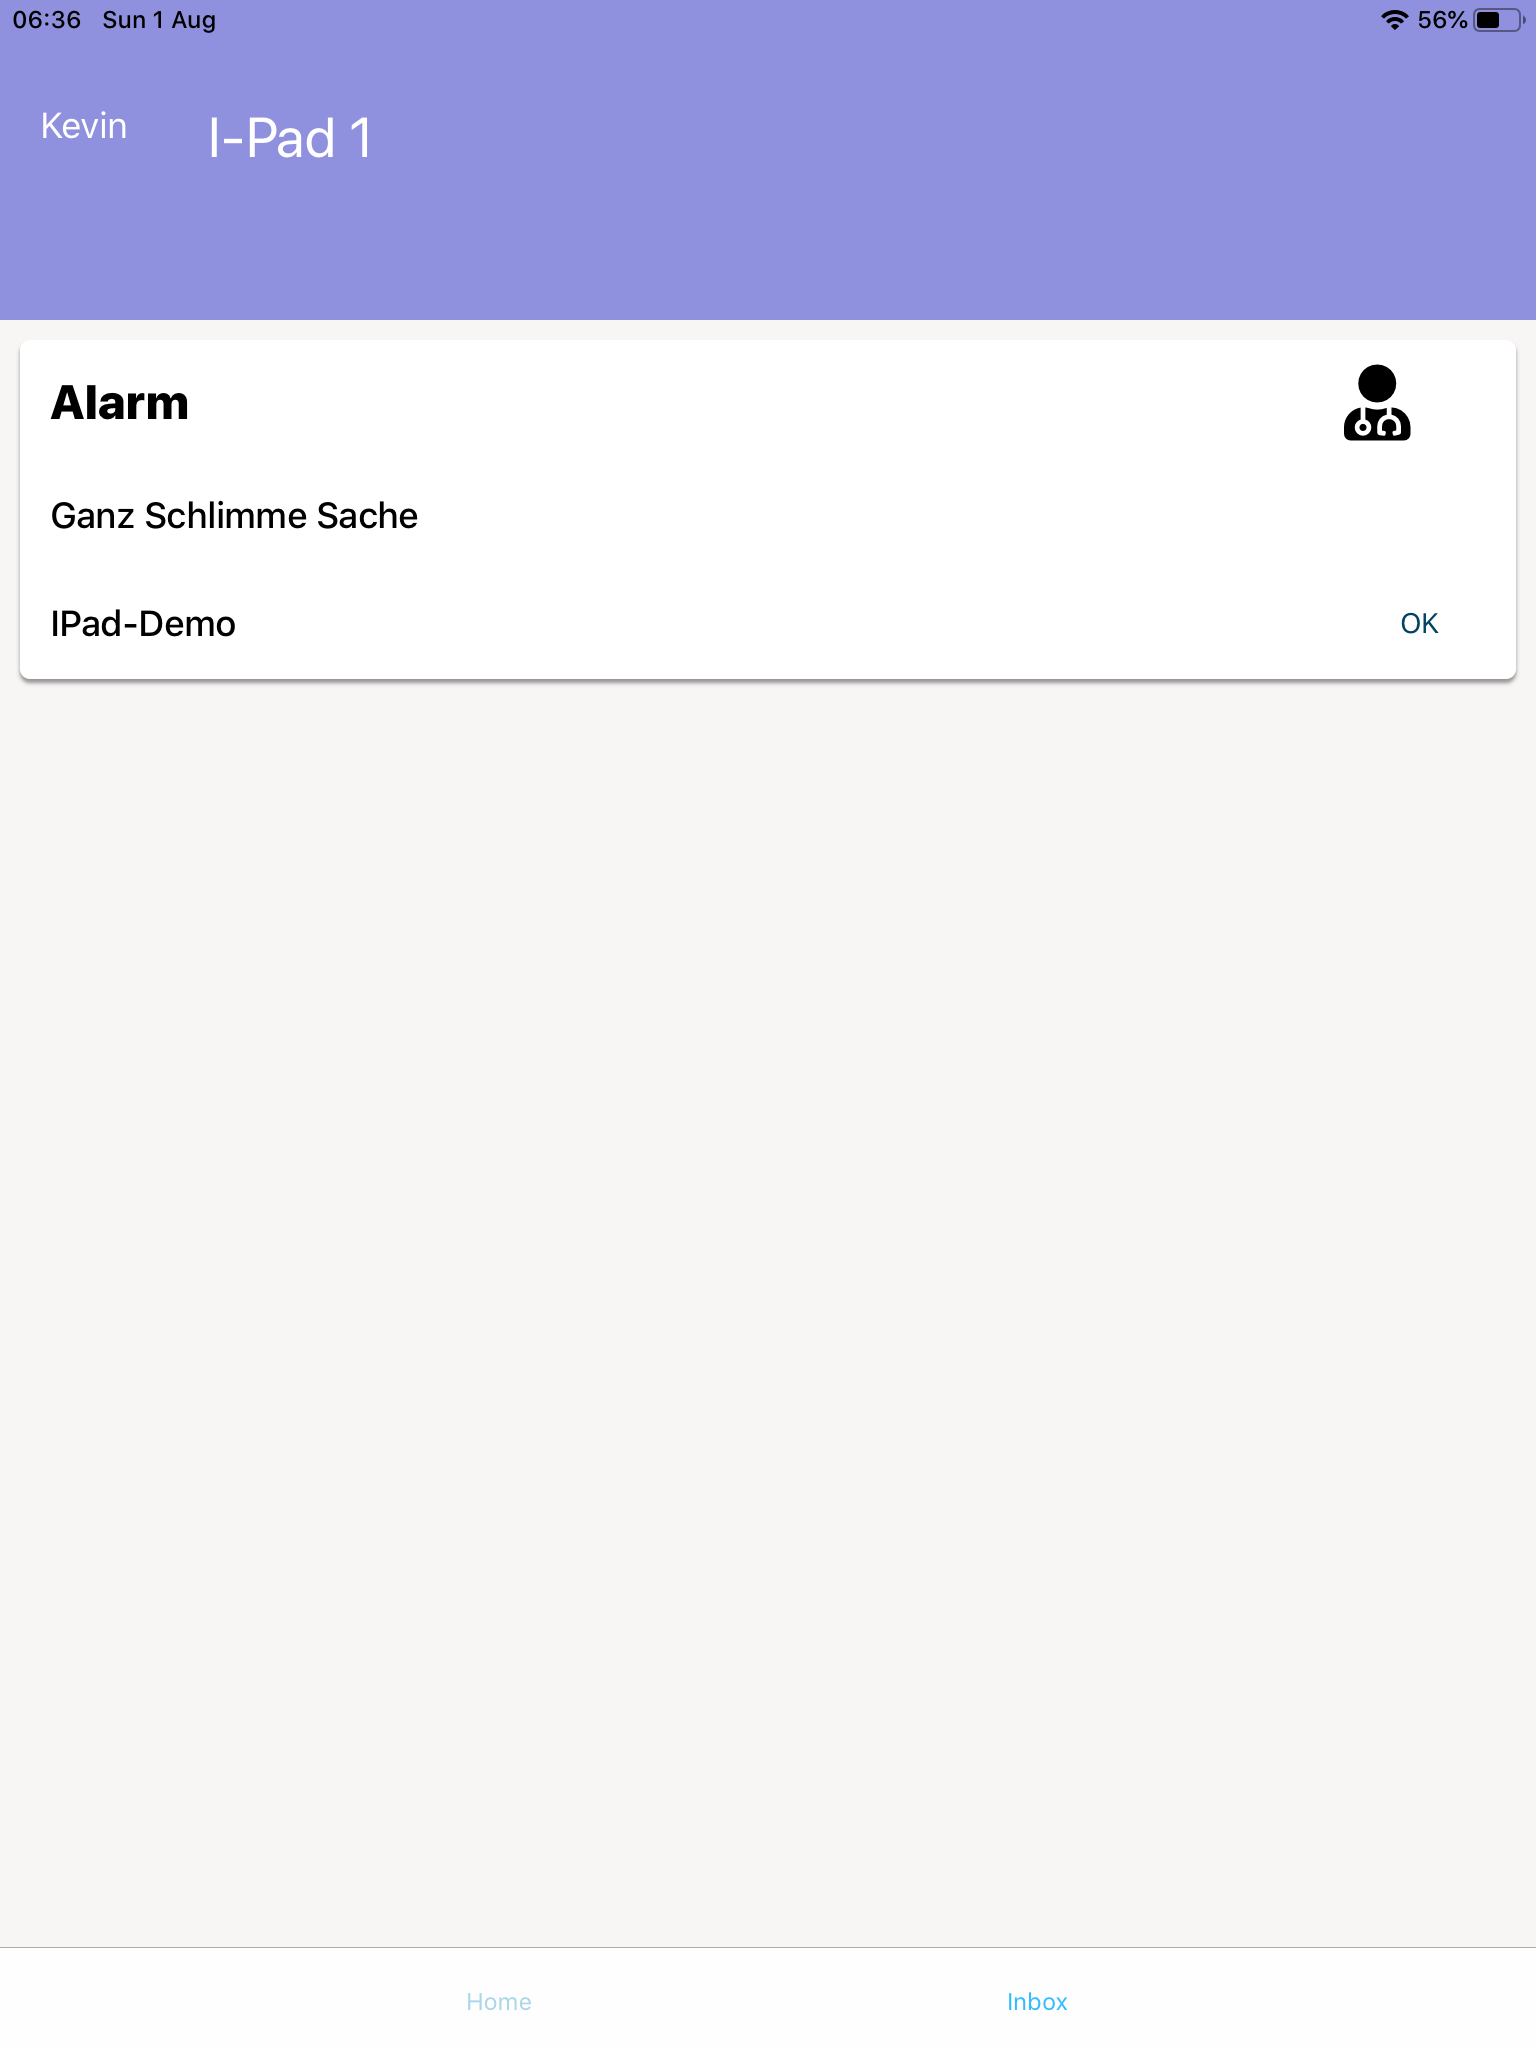
\includegraphics[width=\textwidth]{graphics/screenshots/mobileclient/screenshots-inbox}
        \caption{Inbox}
    \end{minipage}
    \hfill
    \begin{minipage}[b]{0.4\textwidth}
        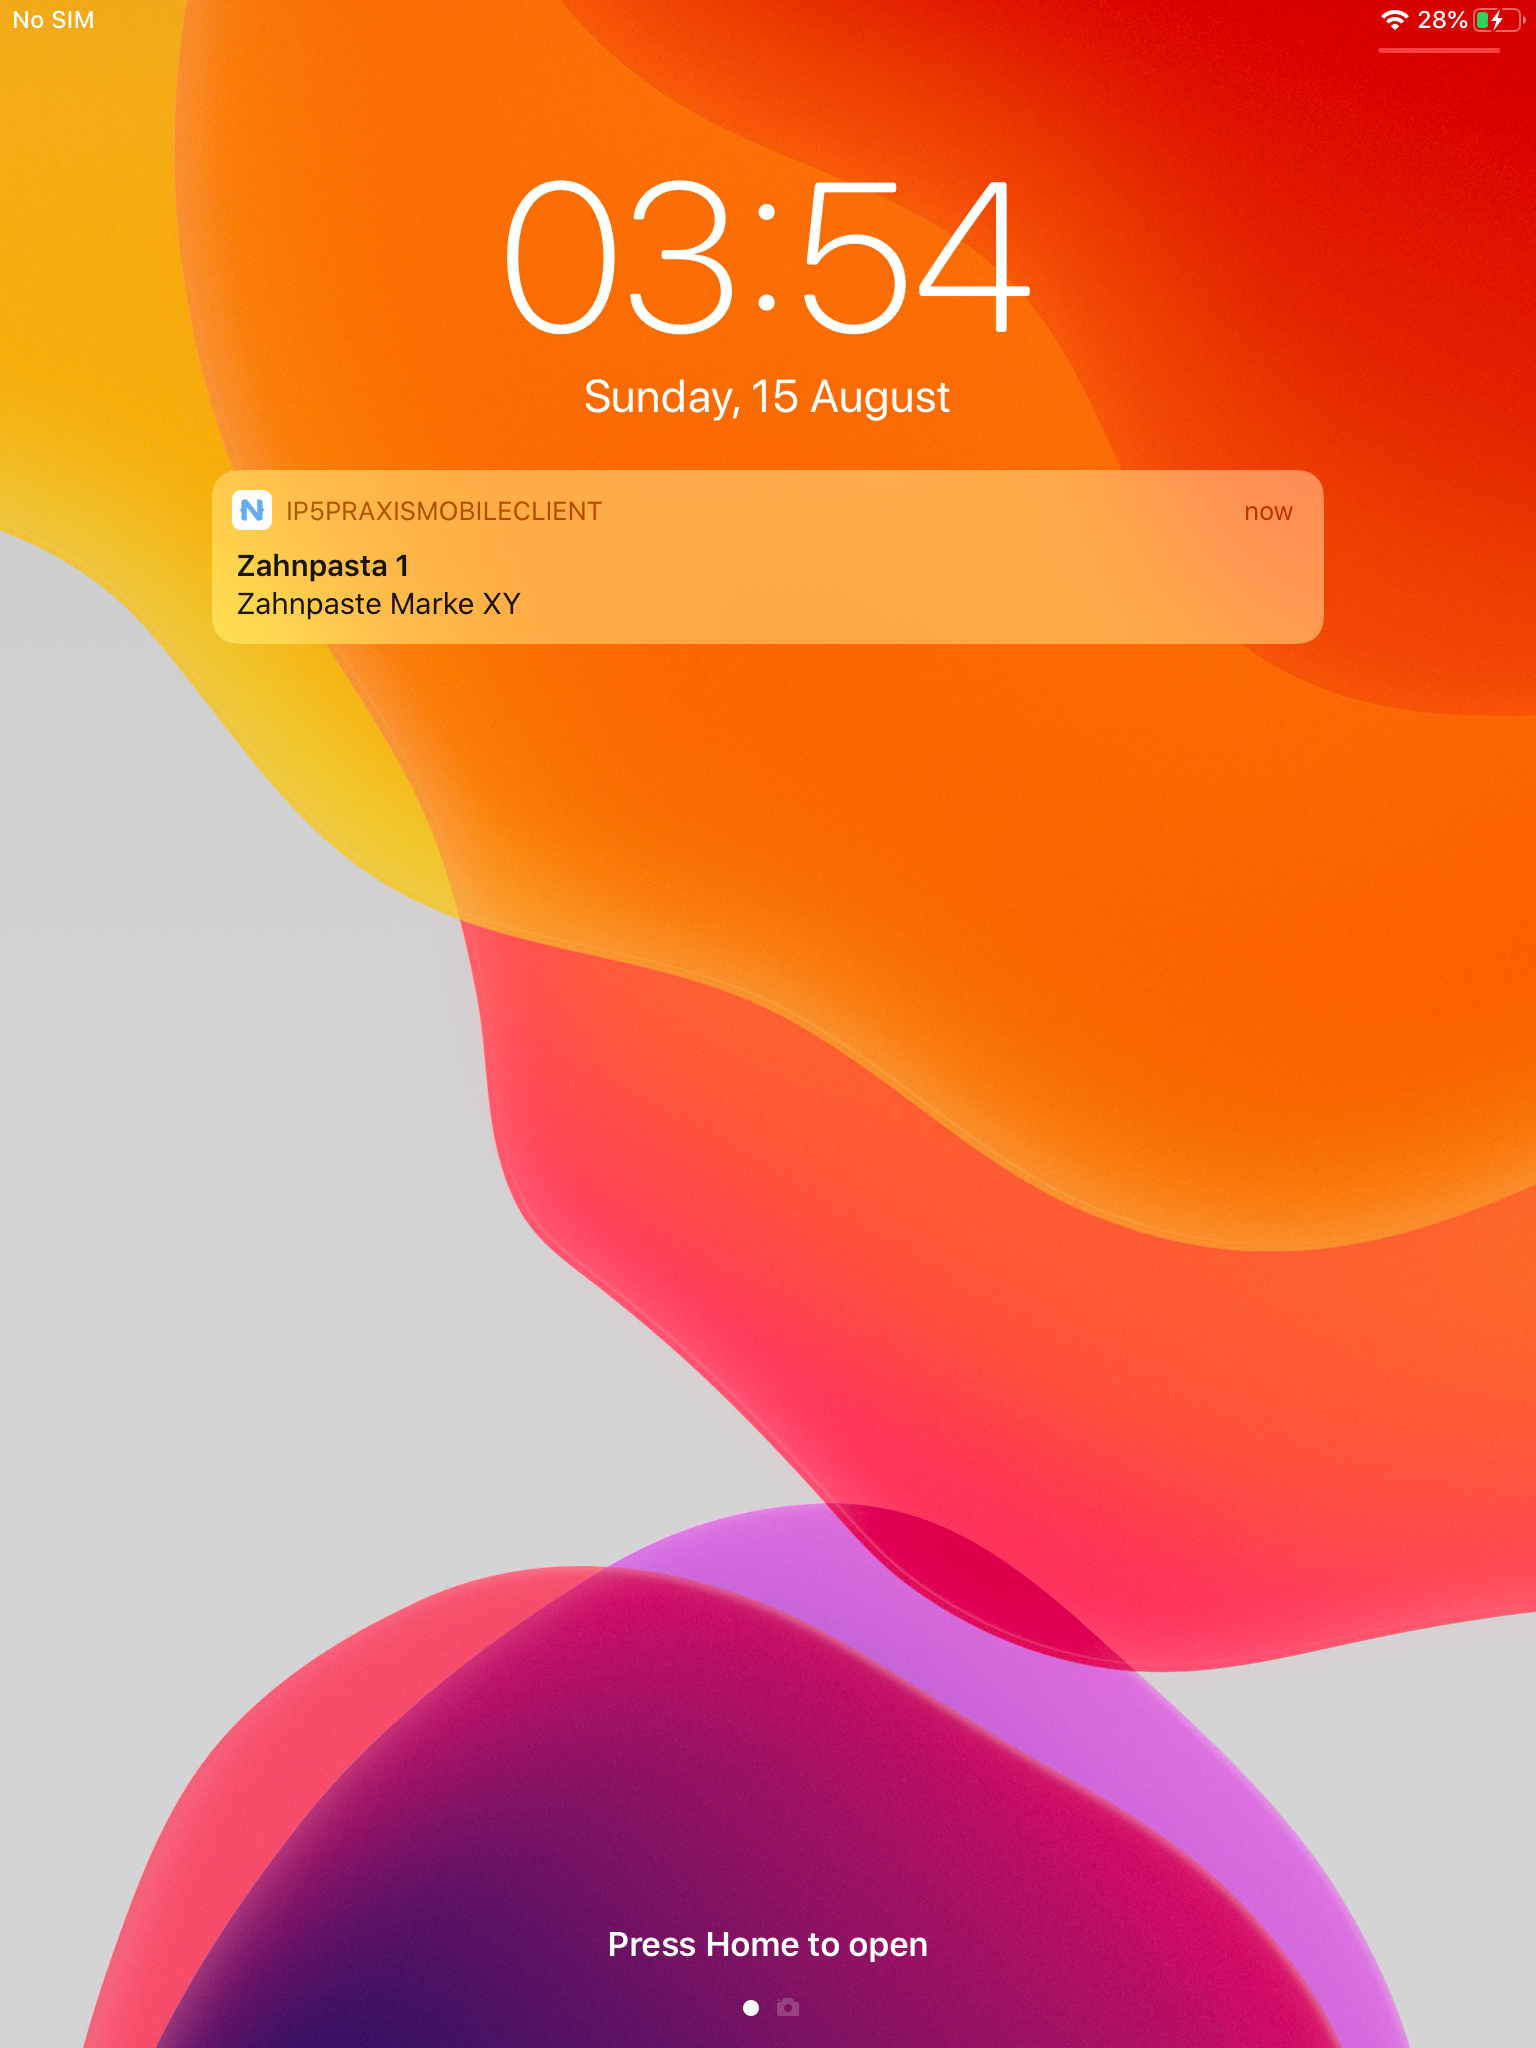
\includegraphics[width=\textwidth]{graphics/screenshots/mobileclient/screenshot-push}
        \caption{Push Benachrichtigung}
    \end{minipage}
    \label{fig:MobileClient-Screens3}
\end{figure}

\clearpage



\subsection{Cloud Service}\label{subsec:cloud-service}

\subsubsection{Architektur}

Es gibt deren Domänen 2. Configuration und Notification.

So quasi als ob man 2 Microservices haben kann. Aber wär halt doof das für den stand jetzt schon so zu trennen, deshalb vorerst mal erst ein einzelnes.

\clearpage

\subsubsection{Domänenmodell}


Für die beiden Domänen gibt es natürlich auch so n paar Diagramme. Die gibts jetzt hier:


\subsubsection*{Domäne Configuration}

\begin{figure}[h]
    \centering
    \begin{minipage}[b]{1.0\textwidth}
        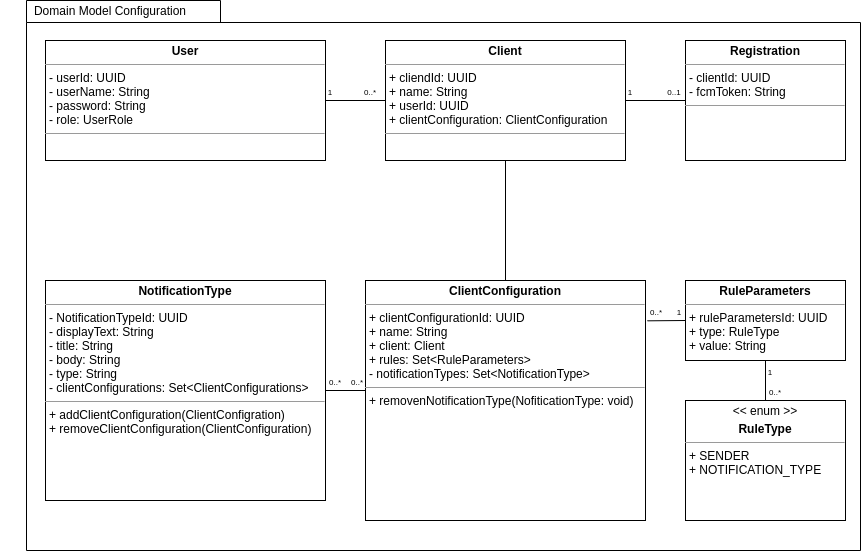
\includegraphics[width=\textwidth]{graphics/Class_Configuration_Domain}
        \caption{Domänenmodell Configuration}
    \end{minipage}
\end{figure}

\clearpage
\subsubsection*{Domäne Notification}

\begin{figure}[h]
    \centering
    \begin{minipage}[b]{1.0\textwidth}
        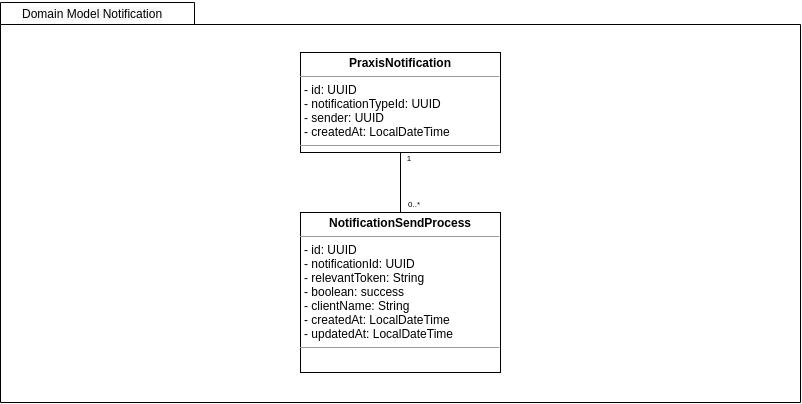
\includegraphics[width=\textwidth]{graphics/Class_Notification_Domain}
        \caption{Domänenmodell Notification}
    \end{minipage}
\end{figure}

\clearpage
\subsubsection*{Rules Engine}

Strategy Pattern mit Spring is noch nice.

\begin{figure}[h]
    \centering
    \begin{minipage}[b]{1.0\textwidth}
        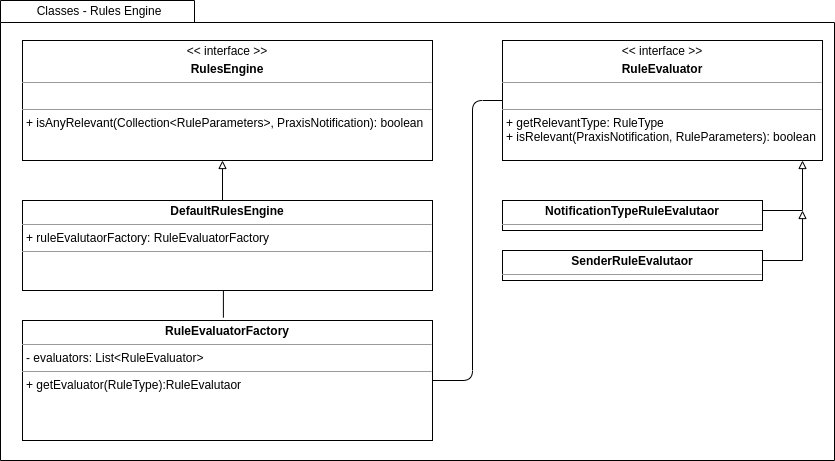
\includegraphics[width=\textwidth]{graphics/Class_Configuration_RulesEngine}
        \caption{Klassendiagramm Rules Engine}
    \end{minipage}
\end{figure}



\clearpage
\subsubsection{API}

S gibt da n paar controller und die brauchen ein paar services.

\clearpage
\subsubsection{Laufzeitmodell}

\clearpage

\subsubsection{Admin UI}

Das Admin UI bietet Praxisverantwortlichen die Möglichkeit die Konfiguration des Praxisrufsystems zu verwalten.
Da nur Praxisverantworliche das Admin UI verwenden dürfen, ist die Benutzeroberfläche durch ein Login geschützt.
Die entsprechenden Anmeldeinformationen müssen bei Installation des Cloud Services vom Betreiber manuell konfiguriert werden.\footnote{Siehe Anhang D}

\begin{figure}[h]
    \centering
    \begin{minipage}[b]{0.4\textwidth}
        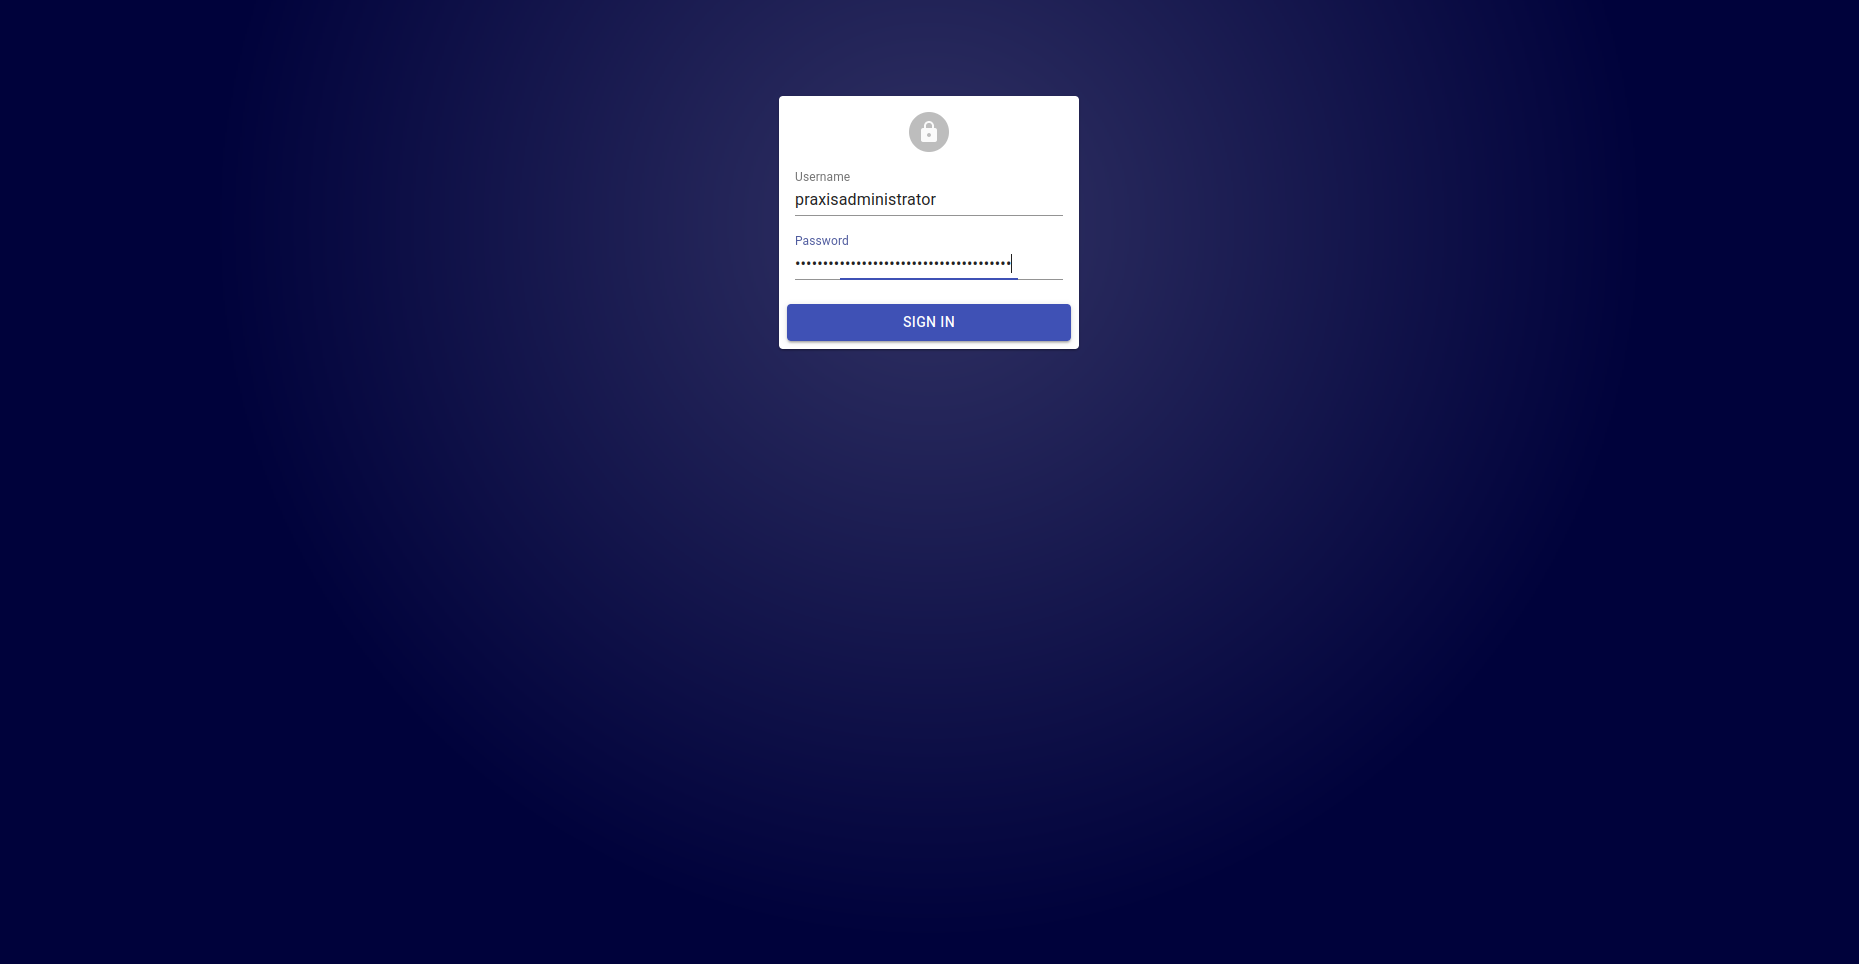
\includegraphics[width=\textwidth]{graphics/screenshots/adminui/login}
        \caption{Login}
    \end{minipage}
    \hfill
    \begin{minipage}[b]{0.4\textwidth}
        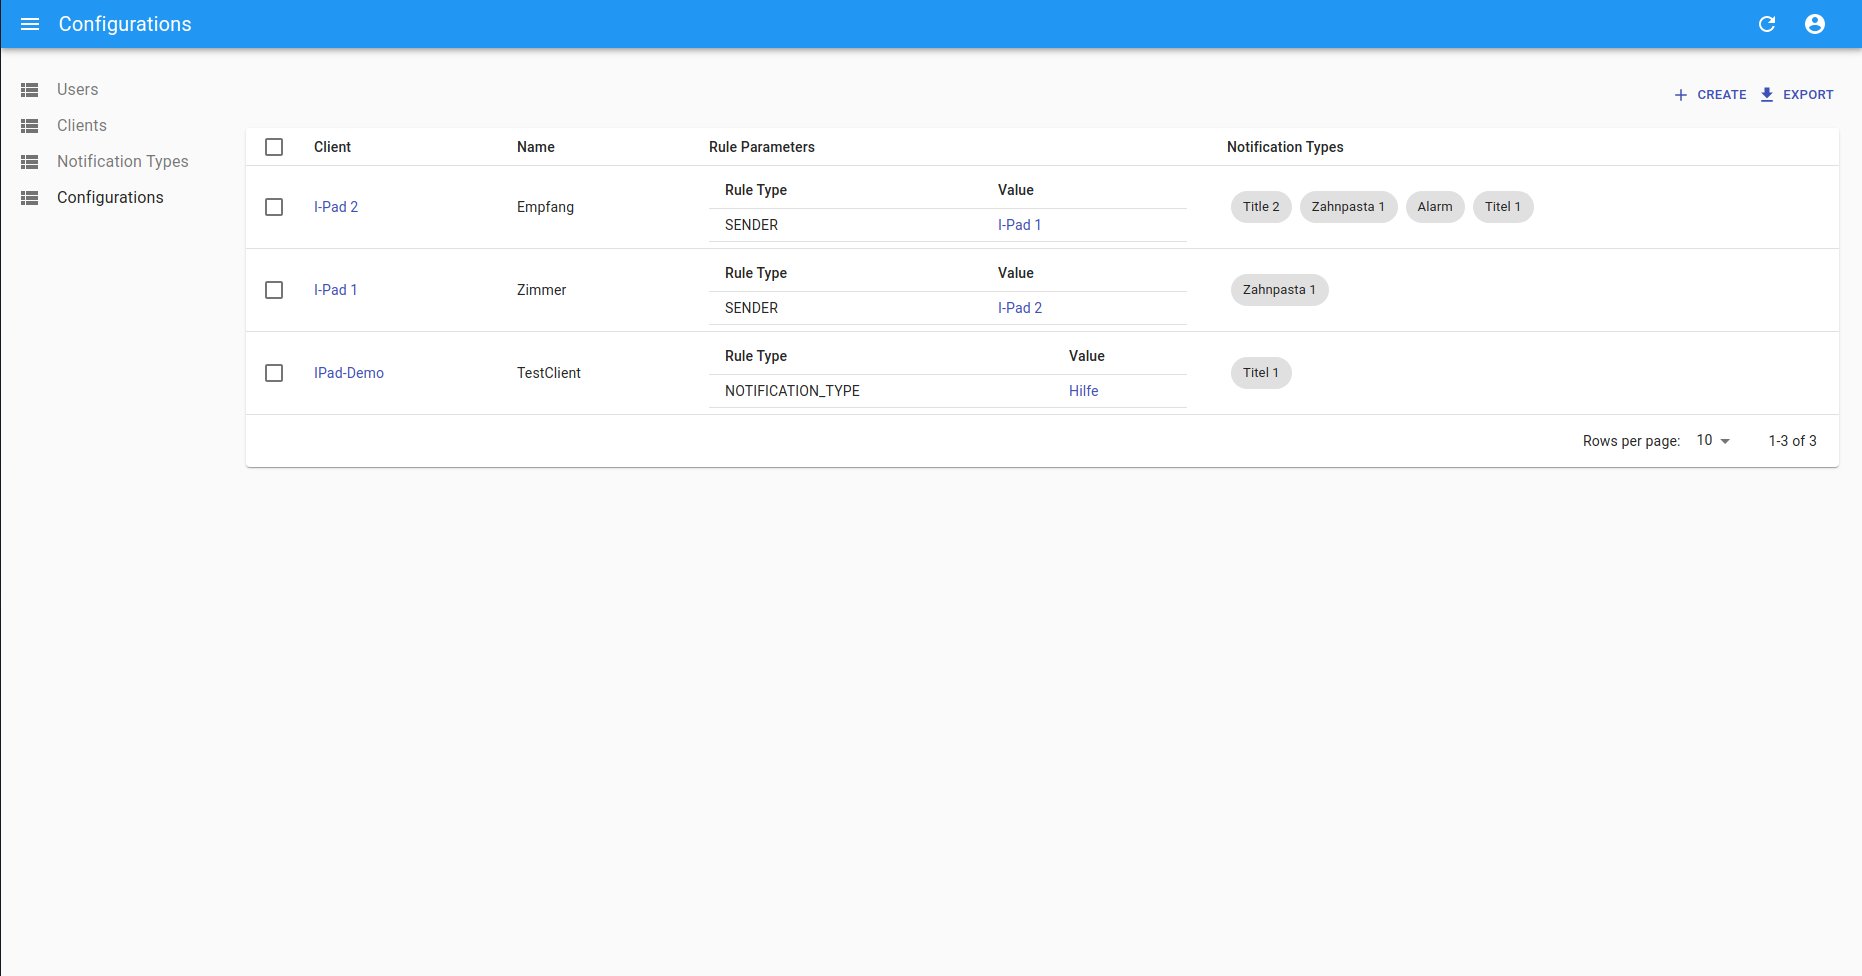
\includegraphics[width=\textwidth]{graphics/screenshots/adminui/configuration-all}
        \caption{Configuration Overview}
    \end{minipage}
    \label{fig:AdminUI-Screens1}
\end{figure}

Das Admin UI beinhaltet vier Bereiche.
Der Bereich Users dient dazu Benutzer zu erstellen, welche sich als Benutzer am Mobile Client anmelden können.
Unter dem Bereich Clients können Geräte verwaltet werden.
Jeder Client ist eindeutig einem Benutzer zugewiesen.
Im Bereich Notification Types können Benachrichtigungen verwaltet werden.
Hier wird konfiguriert, welchen Text der Button für diese Benachrichtigungen im Mobile Client hat und welchen Inhalt die Benachrichtigung hat, wenn sie versendet wird.
Unter dem Bereich Configurations wird die zentrale Konfiguration eines Clients verwaltet.
Jede Konfiguration wird genau einem Client zugewiesen.
Die Konfiguration beinhaltet eine Liste von Notification Types, welche auf dem zugewiesenen Mobile Client als Versenden Button angezeigt werden.
Weiter definiert die Konfiguration eine Liste von Regel Parametern, welche bestimmen, welche Benachrichtigungen dem zugewiesenen Client weitergeleitet werden.

\begin{figure}[h]
    \centering
    \begin{minipage}[b]{0.4\textwidth}
        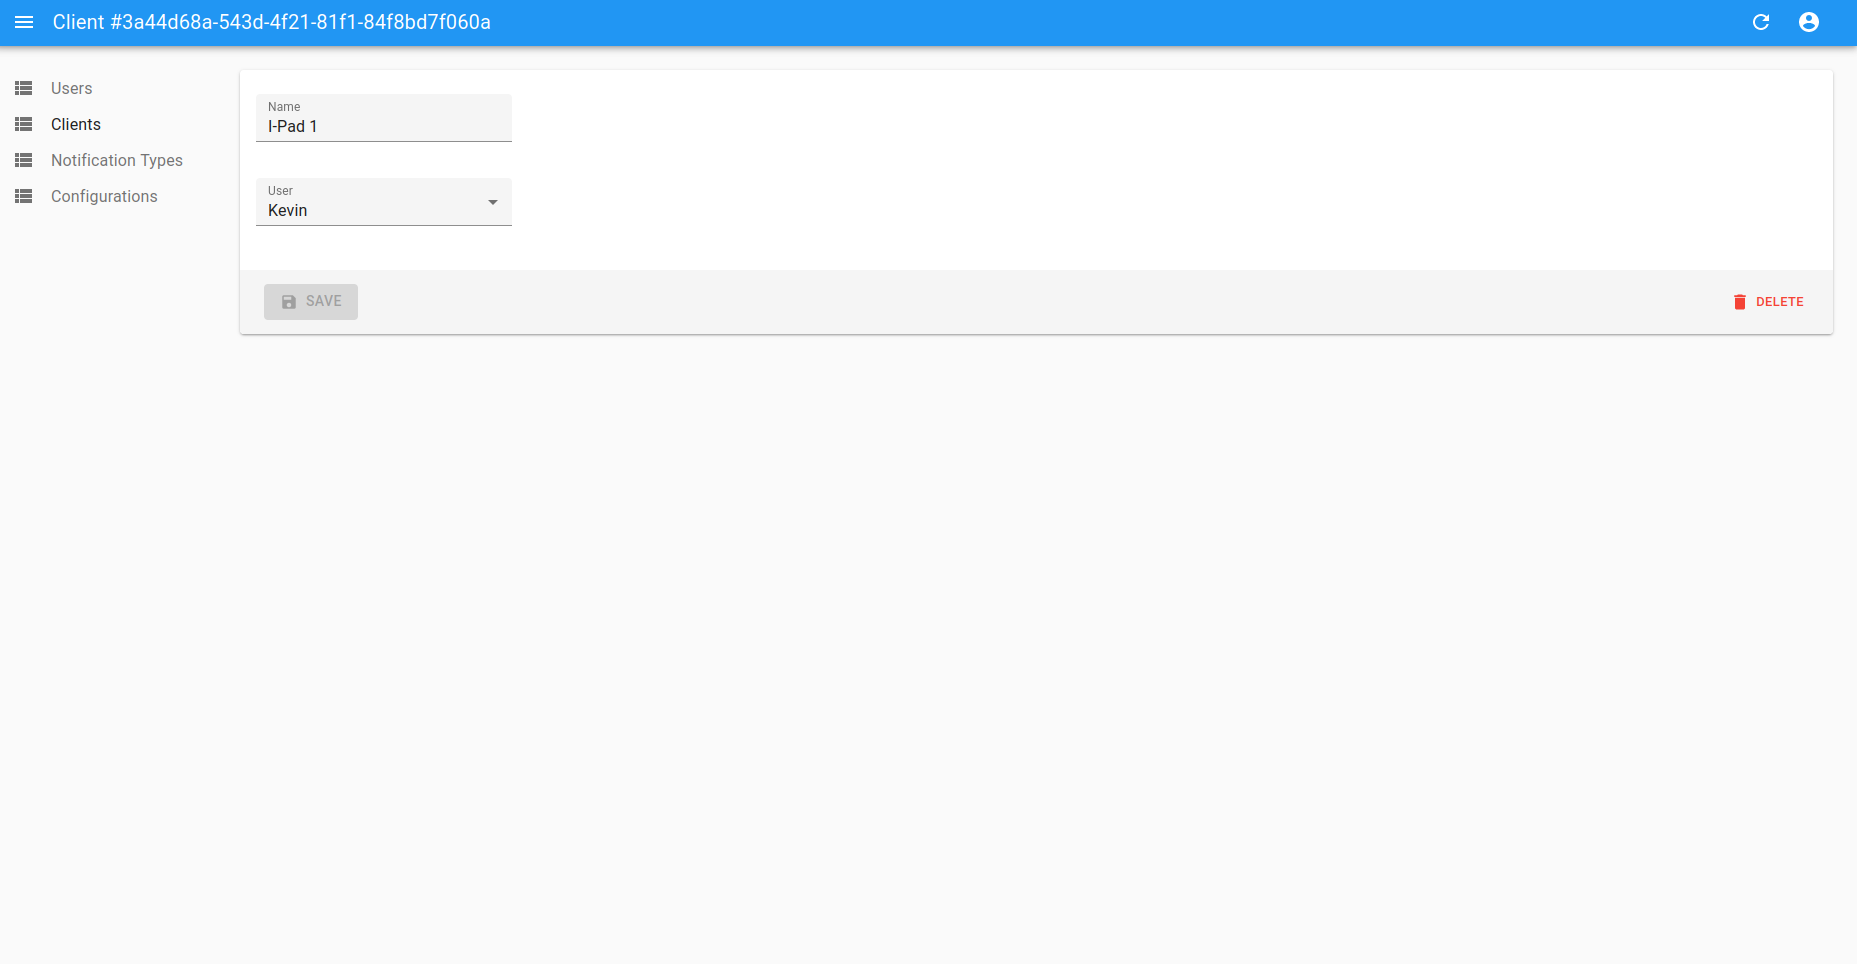
\includegraphics[width=\textwidth]{graphics/screenshots/adminui/configuration}
        \caption{Login}
    \end{minipage}
    \hfill
    \begin{minipage}[b]{0.4\textwidth}
        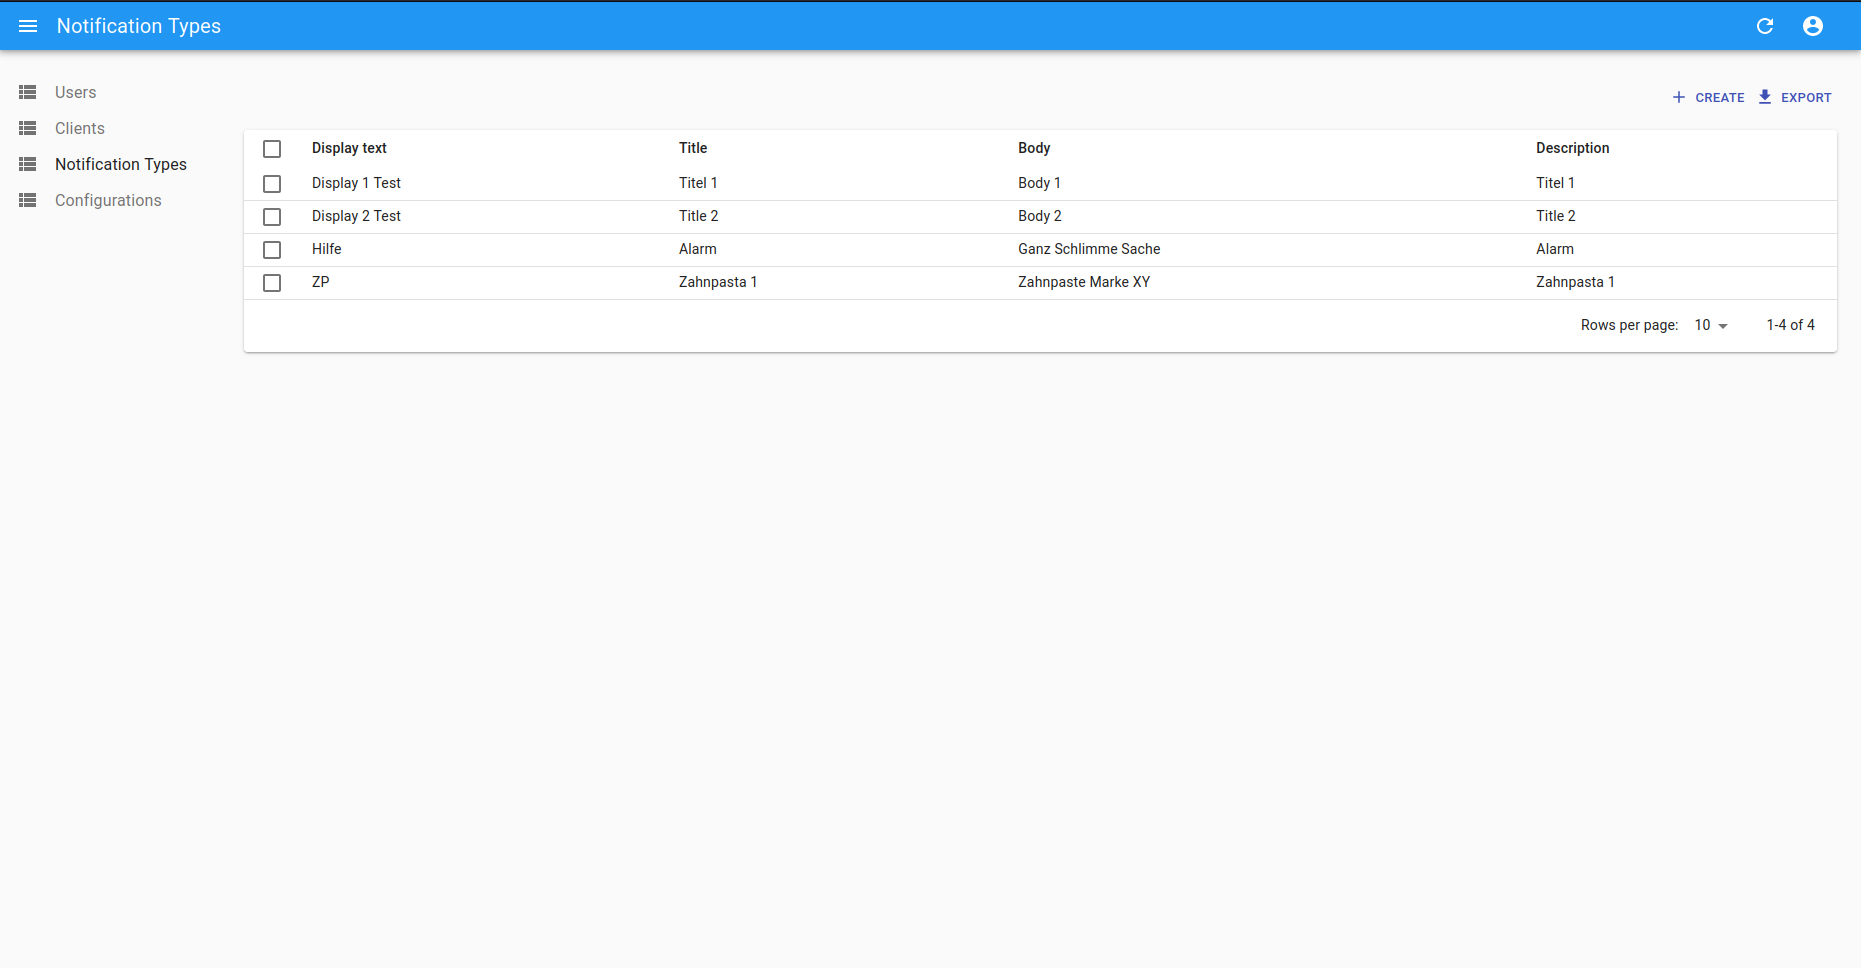
\includegraphics[width=\textwidth]{graphics/screenshots/adminui/notification-type}
        \caption{Configuration Overview}
    \end{minipage}
    \label{fig:AdminUI-Screens2}
\end{figure}

Jeder der Bereiche im Admin UI bietet dem Benutzer die Möglichkeit, den jeweiligen Teil der Konfiguration zu lesen, erstellen, bearbeiten und löschen.
Auf der Startseite jedes Bereiches wird eine Liste mit allen relevanten Einträgen angezeigt.
Mehr Informationen zur Bedienung des Admin UIs befinden sich im Benutzerhandbuch.\footnote{Siehe Anhang C}

\clearpage


\clearpage

\subsection{Proof Of Concept}\label{subsec:poc}

Um sicherzustellen, dass die Anforderungen an das System mit den gewählten Technologien umgesetzt werden können, wird zunächst ein Proof Of Concept implementiert.
Dieser Proof Of Concept hat einen deutlich kleineren Funktionsumfang als das Endprodukt.
Im Wesentlichen muss der Proof Of Concept beweisen, dass es möglich ist mit den gewählten Technologien Benachrichtigungen zu Versenden und zu empfangen.

\subsubsection{Funktionale Anforderungen}

Um dies zu ermöglichen werden die folgenden Features in eingeschränktem Umfang umgesetzt.

\textbf{F01 - Benachrichtigungen Versenden}

Mit dem Proof Of Concept muss es möglich sein, Benachrichtigungen von einem Client zu versenden.
Dementsprechend wird das Szenario "Benachrichtigung versenden" mit den folgenden Einschränkungen umgesetzt:

\begin{itemize}
    \item Es erfolgt kein Login und keine Authentifizierung.
    \item Es gibt nur einen vordefinierten Button.
    \item Es wird immer dieselbe vordefinierte Benachrichtigung versendet.
    \item Es werden keine Empfänger konfiguriert, die Benachrichtigung wird zurück an den Absender versendet.
\end{itemize}


\textbf{F02 - Benachrichtigungen empfangen}

Mit dem Proof Of Concept muss es möglich sein, Benachrichtigungen mit einem Client zu empfangen.
Dementsprechend wird das Szenario "Benachrichtigung empfangen" mit den folgenden Einschränkungen umgesetzt:

\begin{itemize}
    \item Es wird keine Liste von Benachrichtigungen geführt.
    \item Die Benachrichtigung wird in einem einfachen Textfeld im Mobile Client angezeigt.
\end{itemize}


\textbf{F04 - Über Benachrichtigungen Notifizieren}

Mit dem Proof Of Concept muss es möglich sein, über den Einfang von Benachrichtigungen notifiziert zu werden.
Dementsprechend werden die Szenarien "Foreground" und "Background" mit den folgenden Einschränkungen umgesetzt:

\begin{itemize}
    \item Die Notifizierung erfolgt ohne Audio Signal.
\end{itemize}

\clearpage
\subsubsection{Technische Anforderungen}

Damit der Proof Of Concept aussagekräftig ist, müssen die folgenden technischen Anforderungen umgesetzt werden:

\textbf{T01 - IPad Client}

Der für den Proof Of Concept umgesetzte Client muss auf einem IPad funktionieren und alle Anforderungen die an den
Proof Of Concept gestellt werden erfüllen. Kommunikation mit Cloud Service muss funktionieren. Kommunikation mit Messaging Service muss funktionieren.


\textbf{T04 - AWS Platform}

Der Cloud Service muss auf AWS deployed werden. Die Kommunikation zwischen Mobile Client und Cloud Service muss funktionieren.
Die Kommunikation mit Messaging Service muss funktionieren.


\subsubsection{Laufzeitsicht}

Im Wesentlichen muss der Proof Of Concept beweisen, dass es möglich ist mit den gewählten Technologien Benachrichtigungen zu Versenden und zu Empfangen.

Der Benutzer muss den Mobile Client auf dem IPad öffnen können. Aus dem Mobile Client muss der Benutzer über einen Butten eine Benachrichtigung versenden können.
Das Versenden dieser Benachrichtigung erfolgt an den Cloud Service.
Im Rahmen des Proof Of Concept wird eine Benachrichtigung immer an den Sender zurückgesendet. Dabei ist aber wichtig, dass die Benachrichtigung nicht direkt als
Antwort auf die Versenden-Anfrage geschickt wird. Stattdessen muss das Versenden der Benachrichtigung aus dem Cloud Service über den Message Service erfolgen. .

\begin{figure}[h]
    \centering
    \begin{minipage}[b]{1.0\textwidth}
        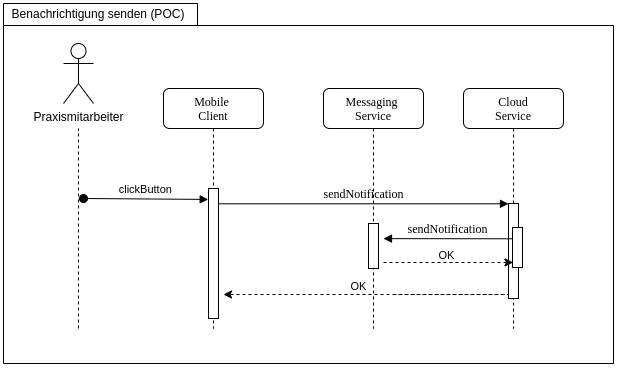
\includegraphics[width=\textwidth]{graphics/Sequence_POC_Send}
        \caption{Proof Of Concept - Benachrichtigung versenden}
    \end{minipage}
\end{figure}

\clearpage


Wurde eine Benachrichtigung über den Message Service an den Mobile Client versendet, muss diese vom Mobile Client empfangen werden.
Als Reaktion auf den Empfang der Benachrichtigung, muss der Inhalt der Benachrichtigung im Mobile Client angezeigt werden. Zudem
muss eine Push Benachrichtigung auf dem Host Gerät erfolgen.

\begin{figure}[h]
    \centering
    \begin{minipage}[b]{1.0\textwidth}
        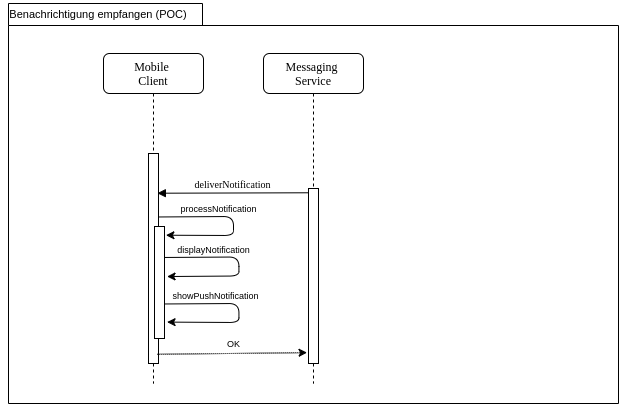
\includegraphics[width=\textwidth]{graphics/Sequence_POC_Receive}
        \caption{Proof Of Concept - Benachrichtigung empfangen}
    \end{minipage}
\end{figure}

\clearpage


    \section{Umsetzung}\label{sec:umsetzung}

    \subsection{Resultate}

        Das Praxisrufsystem wurde wie im Kapitel 5 - Konzept beschrieben umgesetzt.
Es wurden die drei Komponenten Mobile Client, Cloud Service und Admin UI implementiert.
Über den angebundenen Messaging Service Firebase Messaging ist es möglich, Benachrichtigungen zwischen Mobile Clients zu versenden.
Cloud Service und Admin UI ermöglichen es dabei die Benachrichtigungen die Versendet werden können und welcher Client welche Benachrichtungen erhalten soll zu konfigurieren.
Weiter wurde mit Amazon Web Services (AWS) eine CI/CD Umgebung aufgebaut, die es erlaubt Cloud Service und das Admin UI zu betreiben und testen.
Diese Umgebung wird dem Kunden als Template dienen, wie er das Praxisrufsystem in der Praxis betreiben kann\footnote{Siehe Anhang Betriebshandbuch}.

Im Rahmen des Projektes wurden damit die Milestones M01 bis M06\footnote{Siehe Kapitel 2.2} erreicht.
Umgesetzt wurden die Milestones mit den folgenden User Stories inklusive aller dazu definierten Features und Szenarien\footnote{Siehe Kapitel 3}:

\begin{itemize}
    \item U01 - Benachrichtigung versenden
    \item U02 - Benachrichtigungen empfangen
    \item U03 - Nur relevante Benachrichtigungen empfangen
    \item U04 - Auf Benachrichtigungen aufmerksam machen
    \item U05 - Verpasste Benachrichtigungen anzeigen
    \item U06 - Fehler beim Versenden von Benachrichtigungen anzeigen
    \item U07 - Konfiguration auf Mobile Client auswählen
    \item U12 - Mehrere Mobile Clients konfigurieren
    \item U13 - Individuelle Konfiguration pro Mobile Client
    \item U14 - Zentrale Konfigurationsverwaltung
    \item T01 - Mobile Client unterstützt IPads
    \item T02 - Mobile Client unterstützt Android Tablets
    \item T03 - Geteilte Code Basis für Android and IOS
    \item T04 - Betrieb mit AWS
\end{itemize}

Die Milestones M06 bis M10 konnten im Rahmen dieses Projektes nicht umgesetzt werden.
Damit sind folgende User Stories ausserhalb des Projektrahmens gefallen:

\begin{itemize}
    \item U08 - Physicher Knopf am Behandlungsstuhl
    \item U09 - Text To Speech für Benachrichtigungen
    \item U10 - Direkte Unterhaltungen zwischen Mobile Clients
    \item U11 - Gruppenunterhaltungen zwischen Mobile Clients
    \item U15 - Konfiguration von direkten Anrufen
    \item U16 - Konfiguration von Gruppenanrufen
\end{itemize}

        \subsubsection{Mobile Client}\label{subsec:mobile-client-realisation}

Dieses Kapitel zeigt die umgesetzten Ansichten des Mobile Clients.
Weitere Informationen zur Bedienung des Mobile Clients sind dem Benutzerhandbuch zu entnehmen\footnote{Siehe Anhang C}.

\subsubsection*{Anmeldung und Konfiguration}

Wird die Mobile Client Applikation zu ersten Mal geöffnet, muss die korrekte Konfiguration geladen werden.
So können Buttons für die benötigten Benachrichtigungen angezeigt und relevante Benachrichtigungen empfangen werden.
In einem ersten Schritt wird dem Benutzer deshalb eine einfache Login-Maske angezeigt.
Darin kann sich der Benutzer mit Benutzername und Passwort anmelden.
War die Anmeldung erfolgreich, werden alle Konfigurationen geladen, die dem Benutzer zur Verfügung stehen.
Die verfügbaren Konfigurationen werden dem Benutzer in einer Liste angezeigt und er wird aufgefordert, die gewünschte Konfiguration auszuwählen.
Nachdem die Auswahl erfolgt ist, wird der Benutzer zur Startseite weitergeleitet.

\begin{figure}[h]
    \centering
    \begin{minipage}[b]{0.4\textwidth}
        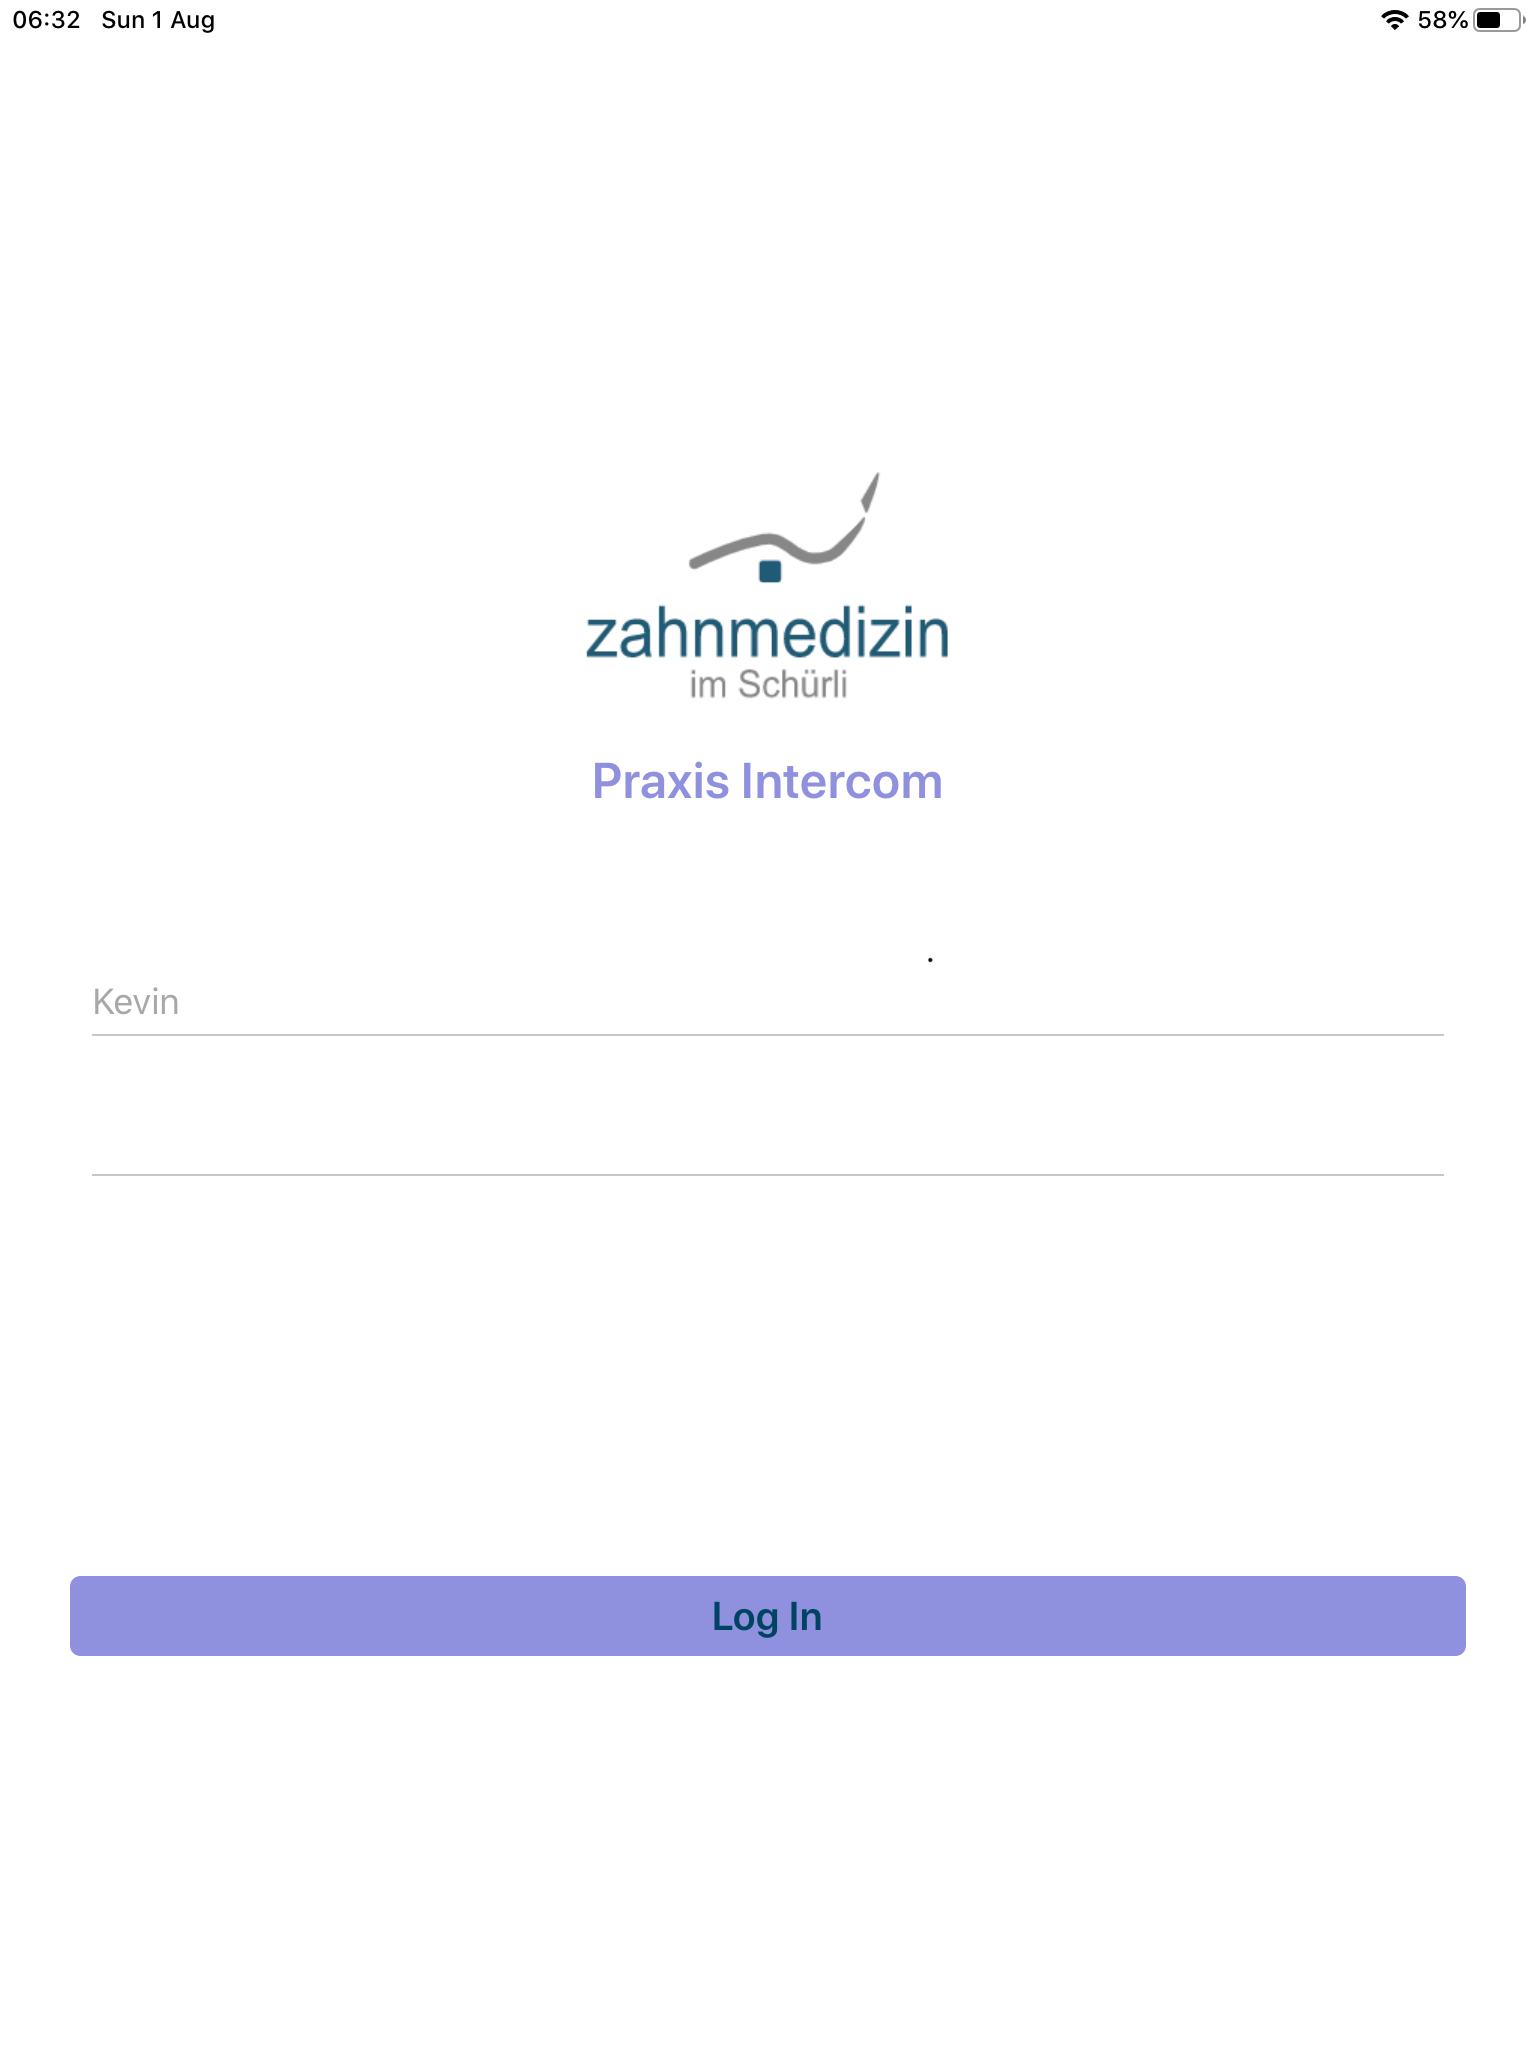
\includegraphics[width=\textwidth]{graphics/screenshots/mobileclient/screenshots-login}
        \caption{Login}
    \end{minipage}
    \hfill
    \begin{minipage}[b]{0.4\textwidth}
        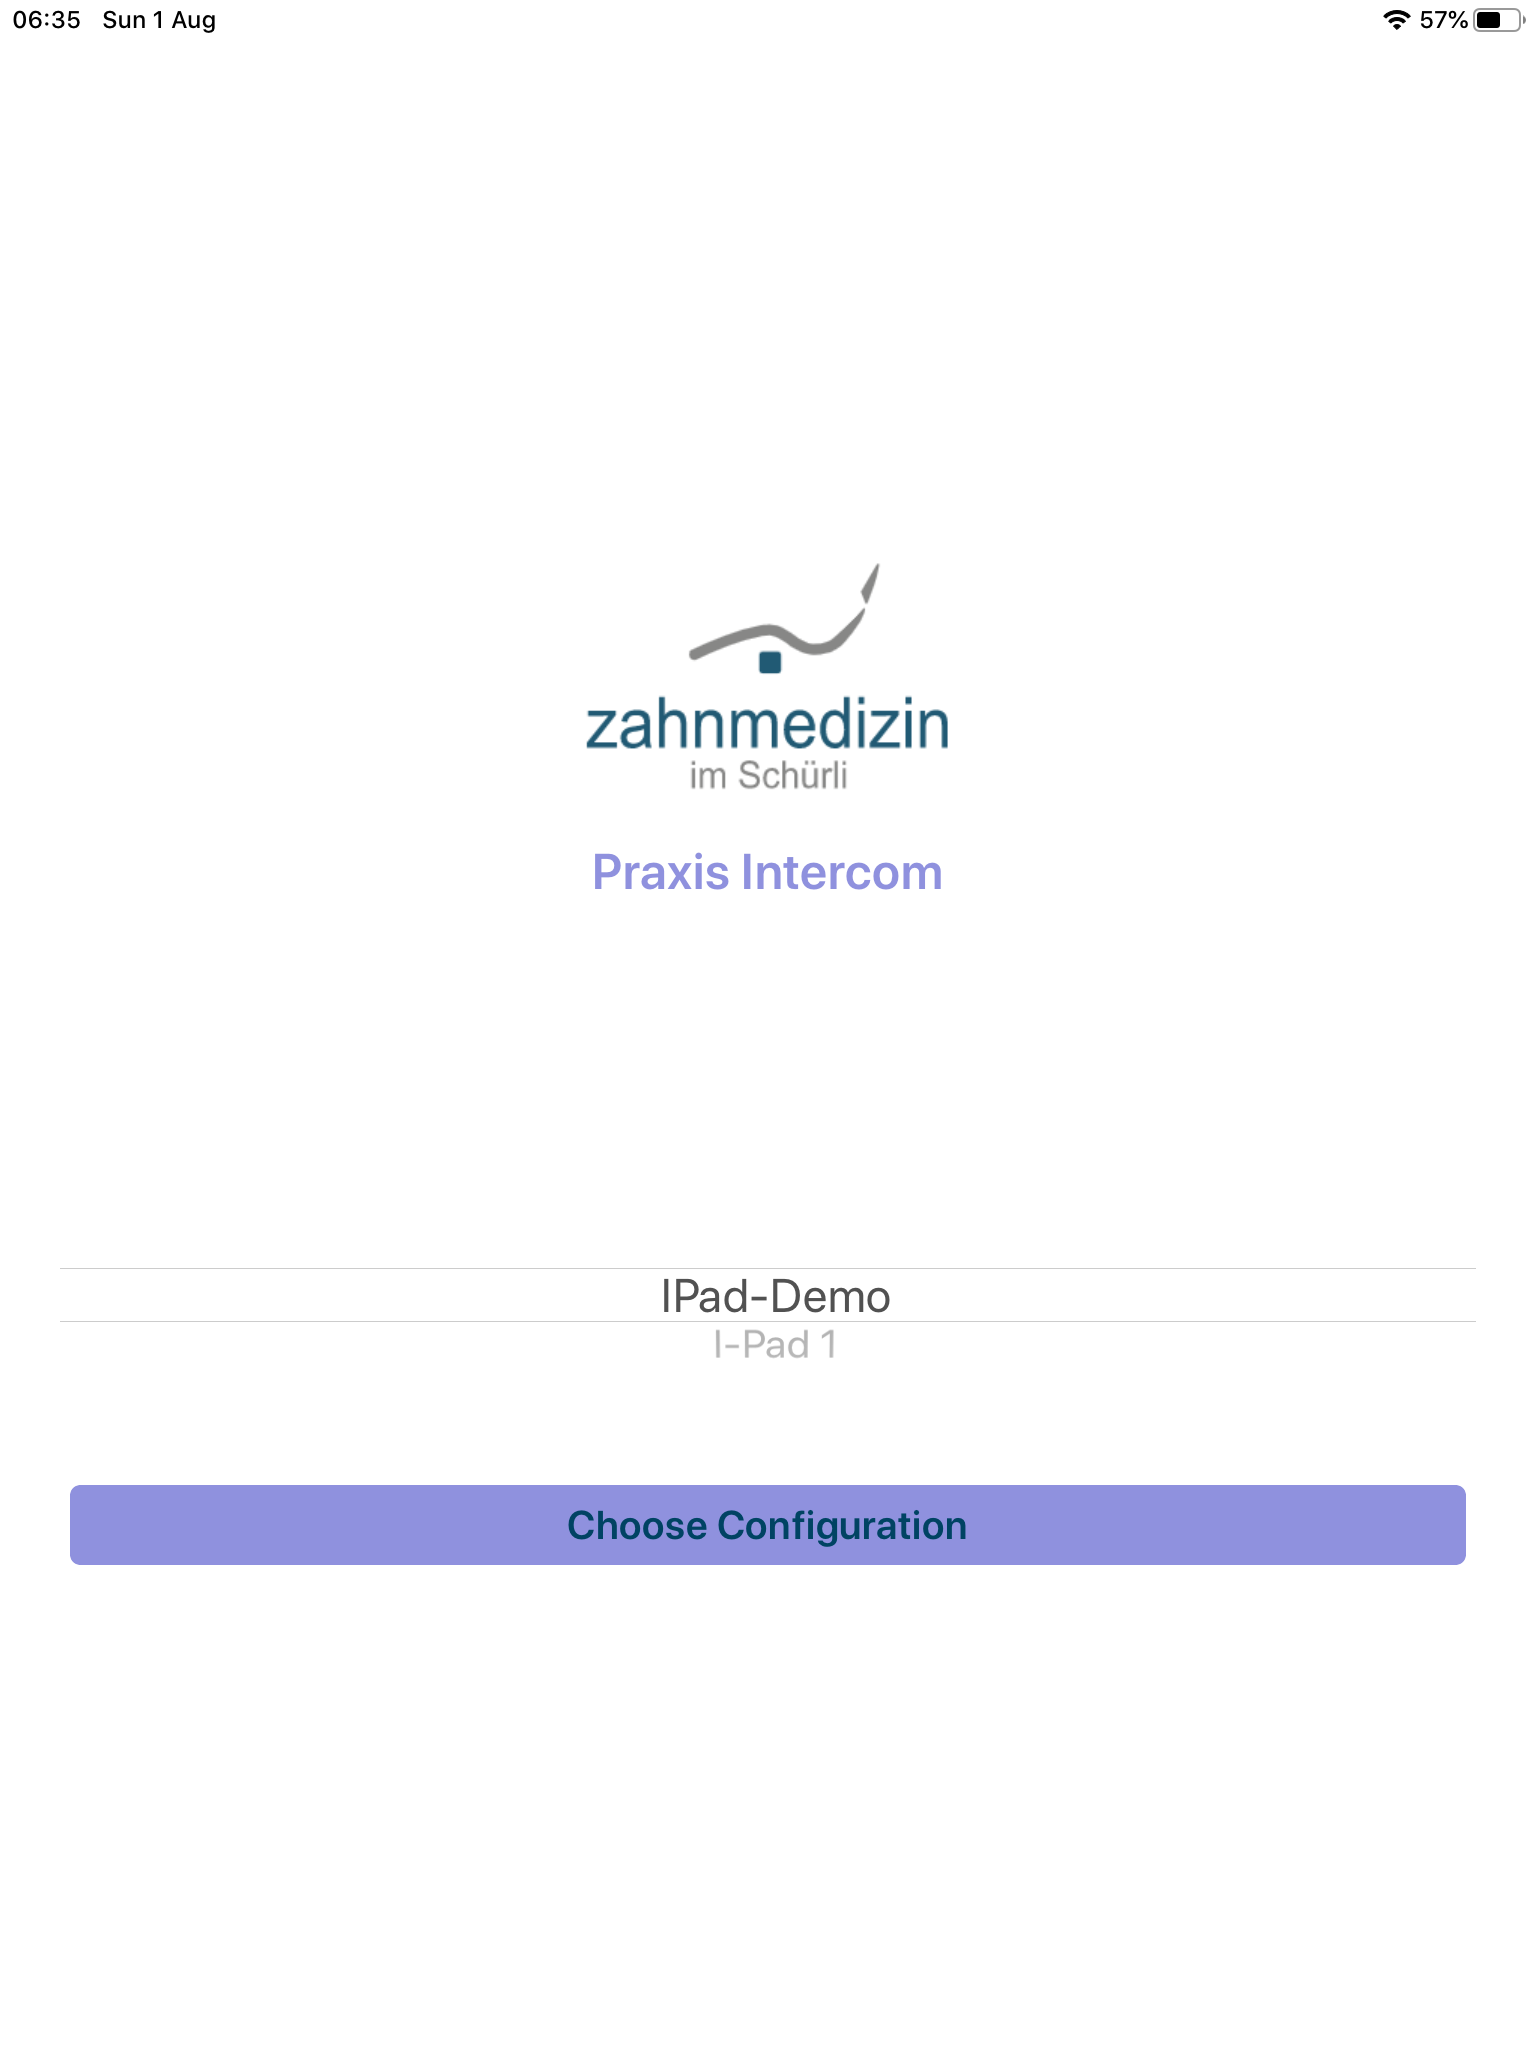
\includegraphics[width=\textwidth]{graphics/screenshots/mobileclient/screenshot-select-config}
        \caption{Konfiguration}
    \end{minipage}
    \label{fig:MobileClient-Screens1}
\end{figure}

\clearpage

\subsubsection*{Benachrichtigungen versenden}

Im Tab Home der Startseite werden Buttons angezeigt, um Benachrichtigungen zu versenden.
Die Buttons werden dynamisch aus der geladenen Konfiguration generiert.
Dabei gibt die Konfiguration den Text vor, der auf dem Button angezeigt wird.
Der Inhalt der Benachrichtigung, die der Button auslöst, ist in der Konfiguration im Cloud Service hinterlegt.

Tippt der Benutzer auf einen der Buttons, wird die entsprechende Benachrichtigung versendet.
Die Vermittlung, an die relevanten Empfänger übernimmt dabei der Cloud Service.
Dieser entscheidet anhand der vorhandenen Konfiguration, welchen Clients die Benachrichtigung zugestellt wird.
Schlägt das Versenden der Benachrichtigung an mindestens einen Empfänger fehl, wird dies dem Benutzer angezeigt.
Der Benutzer hat dann die Möglichkeit, das Versenden an diese Empfänger wiederholen.

\begin{figure}[h]
    \centering
    \begin{minipage}[b]{0.4\textwidth}
        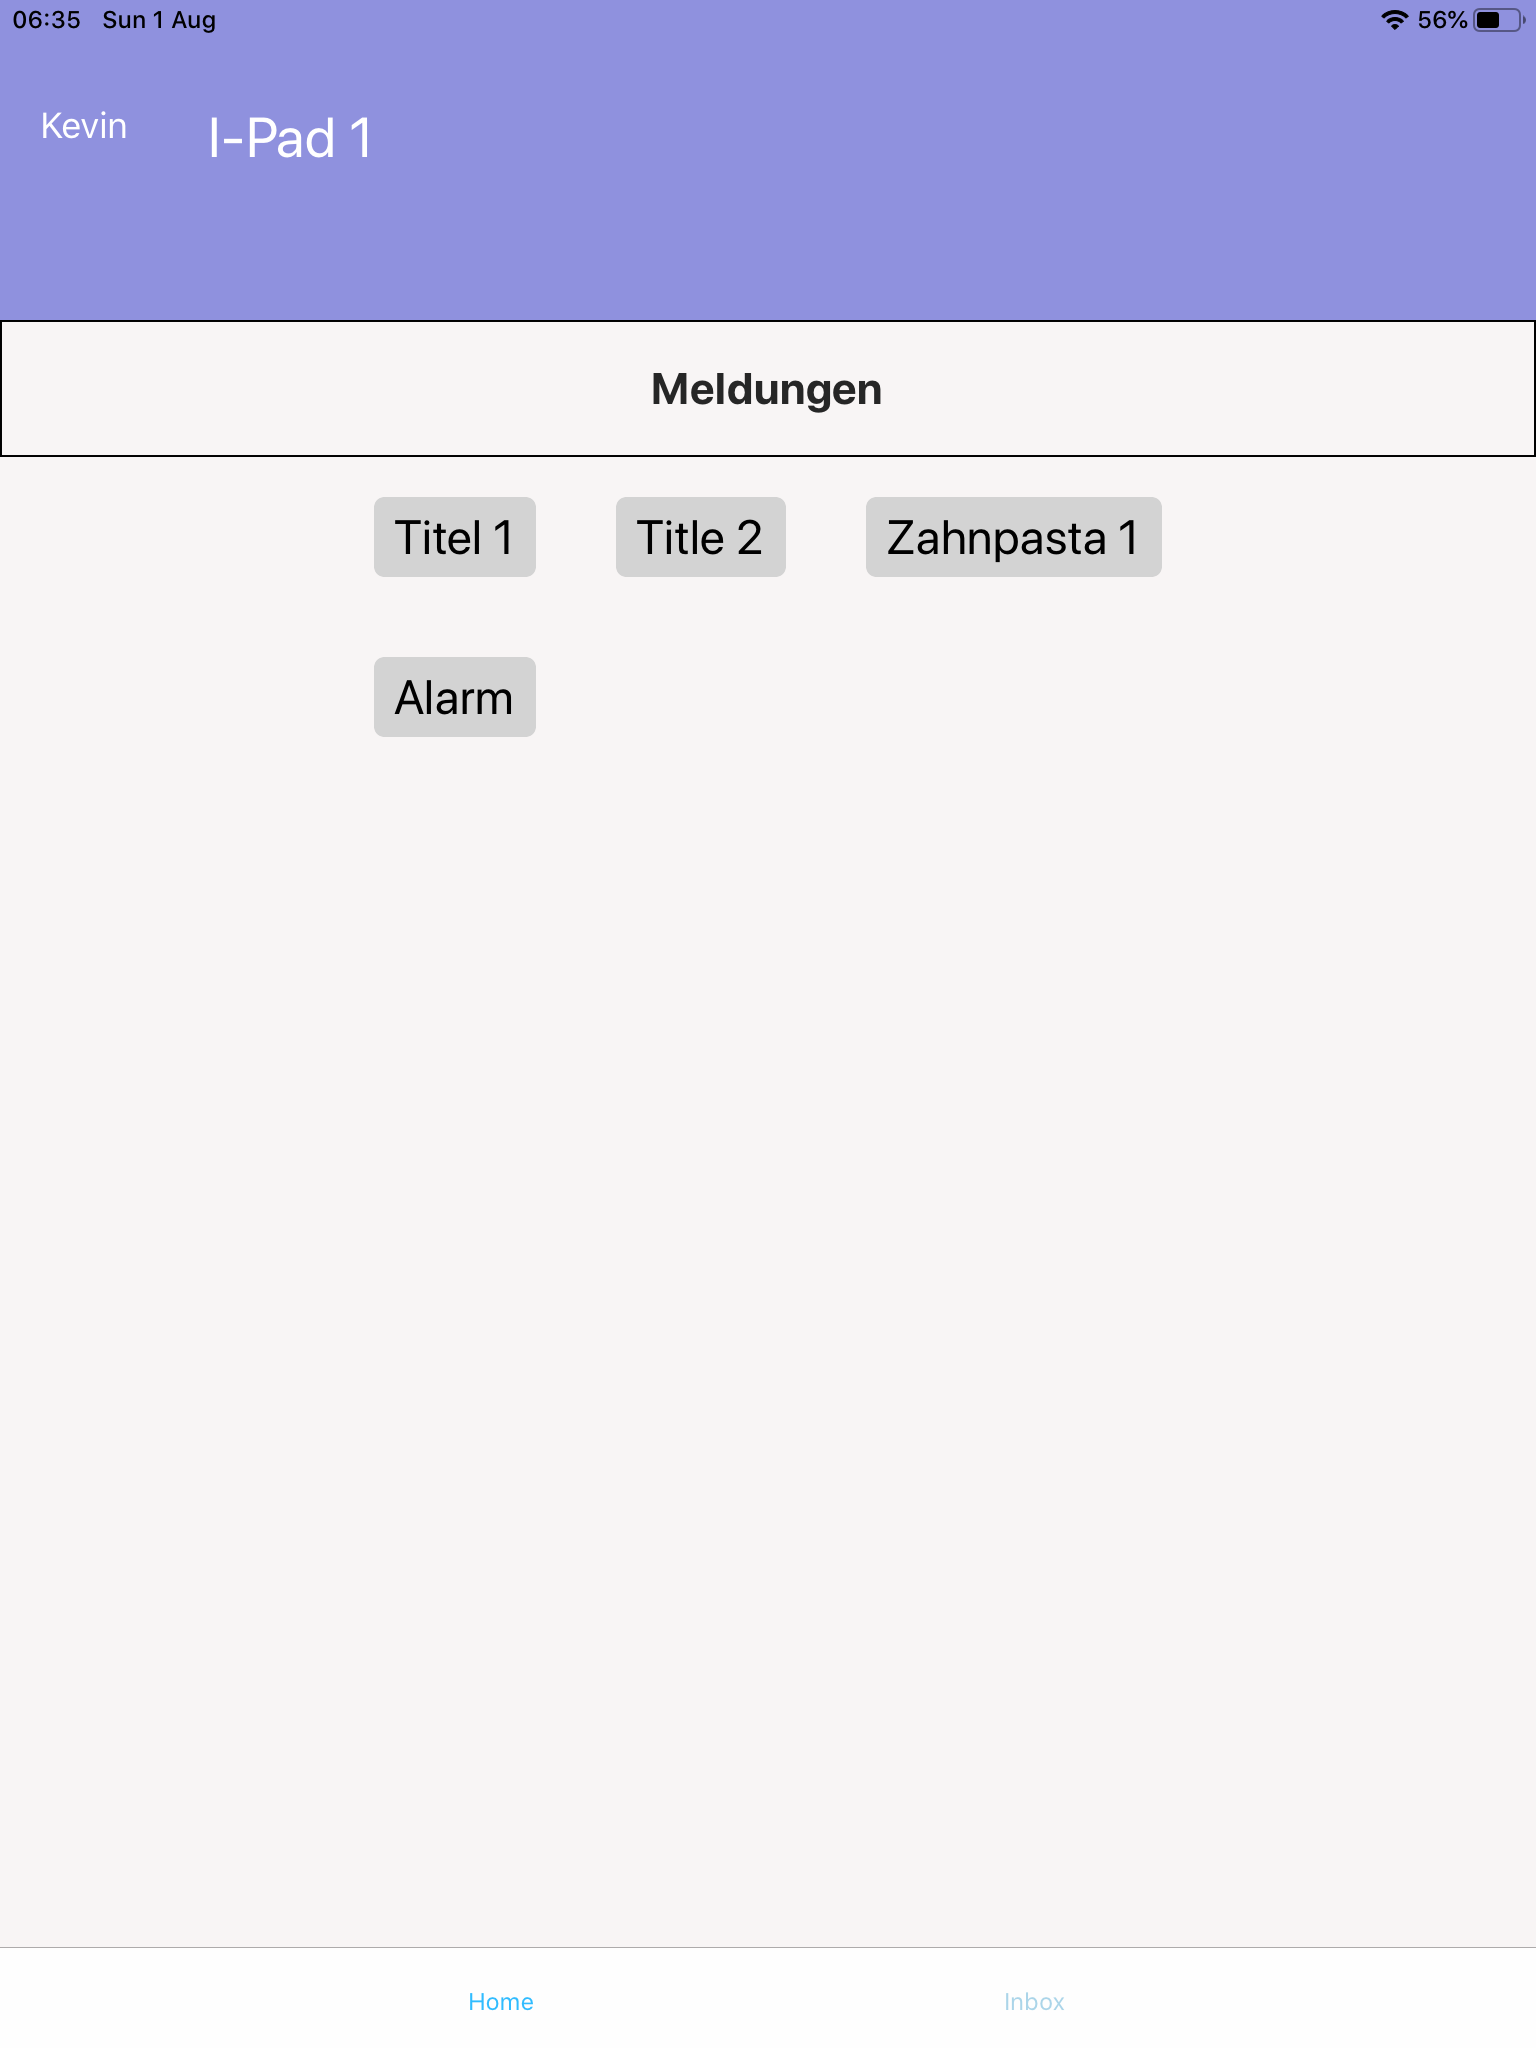
\includegraphics[width=\textwidth]{graphics/screenshots/mobileclient/screenshot-homescreen}
        \caption{Home}
    \end{minipage}
    \hfill
    \begin{minipage}[b]{0.4\textwidth}
        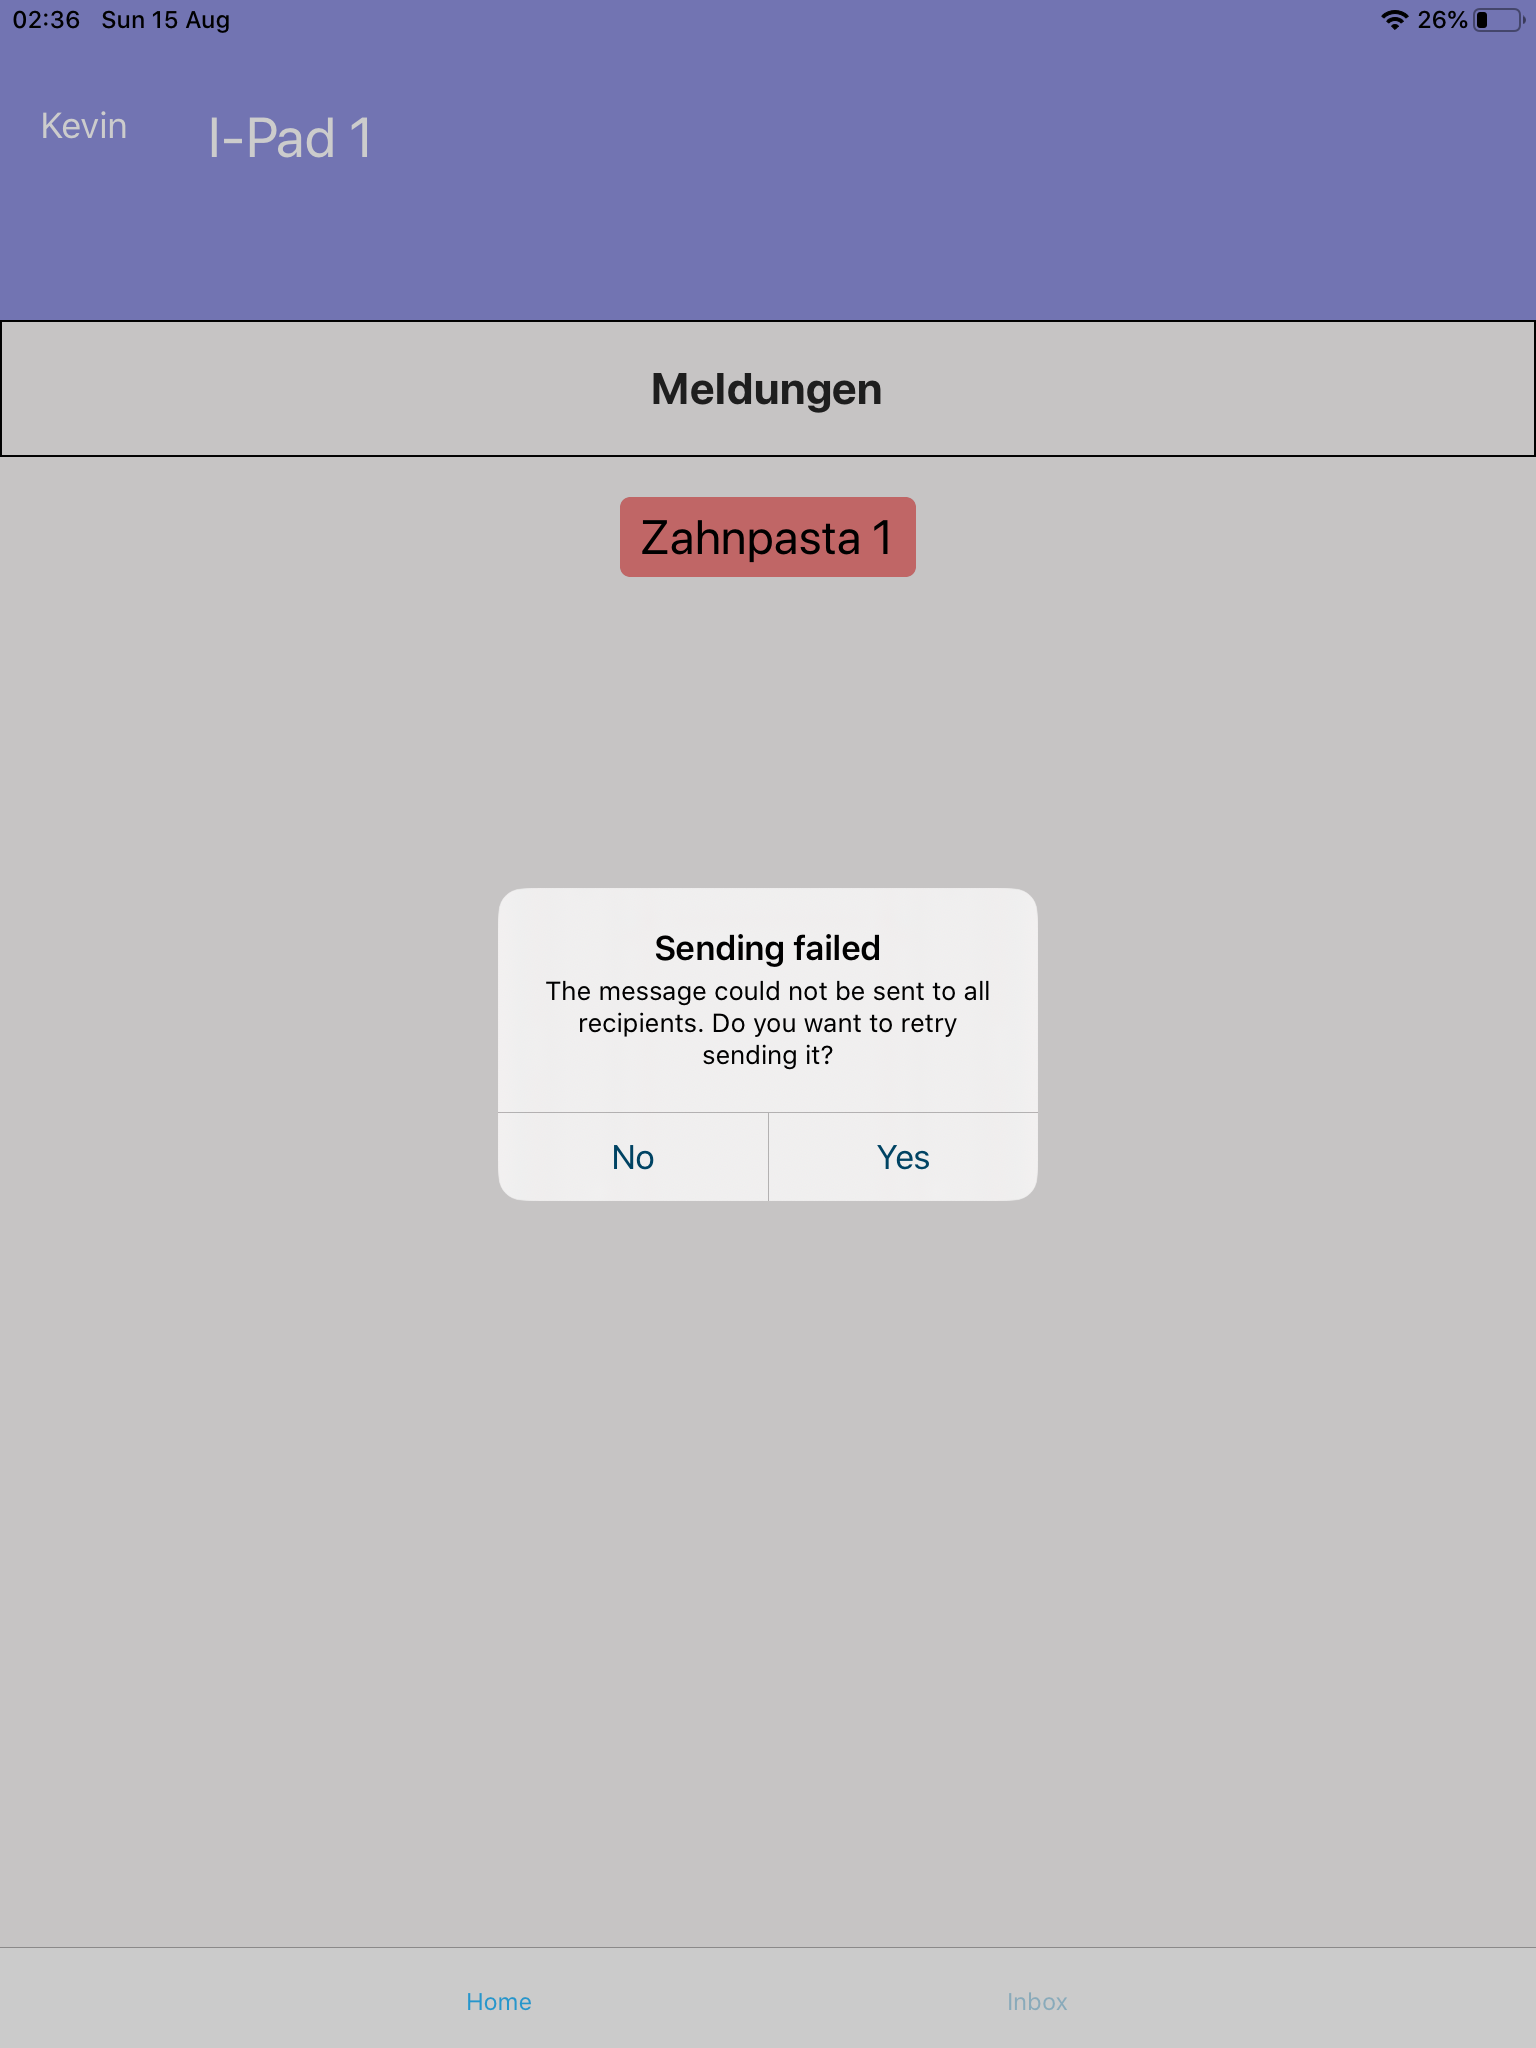
\includegraphics[width=\textwidth]{graphics/screenshots/mobileclient/screenshot-retry}
        \caption{Retry}
    \end{minipage}
    \label{fig:MobileClient-Screens2}
\end{figure}

\clearpage

\subsubsection*{Benachrichtigungen empfangen}

Wurde eine Benachrichtigung empfangen, ertönt ein Audio Signal und die Benachrichtigung ist im Tab Inbox auf der Startseite ersichtlich.
Durch Klick auf einen der Einträge in der Liste, kann der Benutzer die empfangene Benachrichtigung quittieren.
Wenn die Inbox Benachrichtigungen enthält, die nicht quittiert wurden, wiederholt der Client im Abstand von 30 Sekunden.
Die Quittierung von Benachrichtigungen erfolgt nur lokal auf dem Gerät.
Der Versender wird nicht über die Quittierung benachrichtigt.
Wurde eine Benachrichtigung im Hintergrund empfangen, wird diese als Push-Benachrichtigung auf dem Gerät angezeigt.
Auch wenn die Benachrichtigung im Hintergrund empfangen wurde, wird diese in der Inbox angezeigt.

\begin{figure}[h]
    \centering
    \begin{minipage}[b]{0.4\textwidth}
        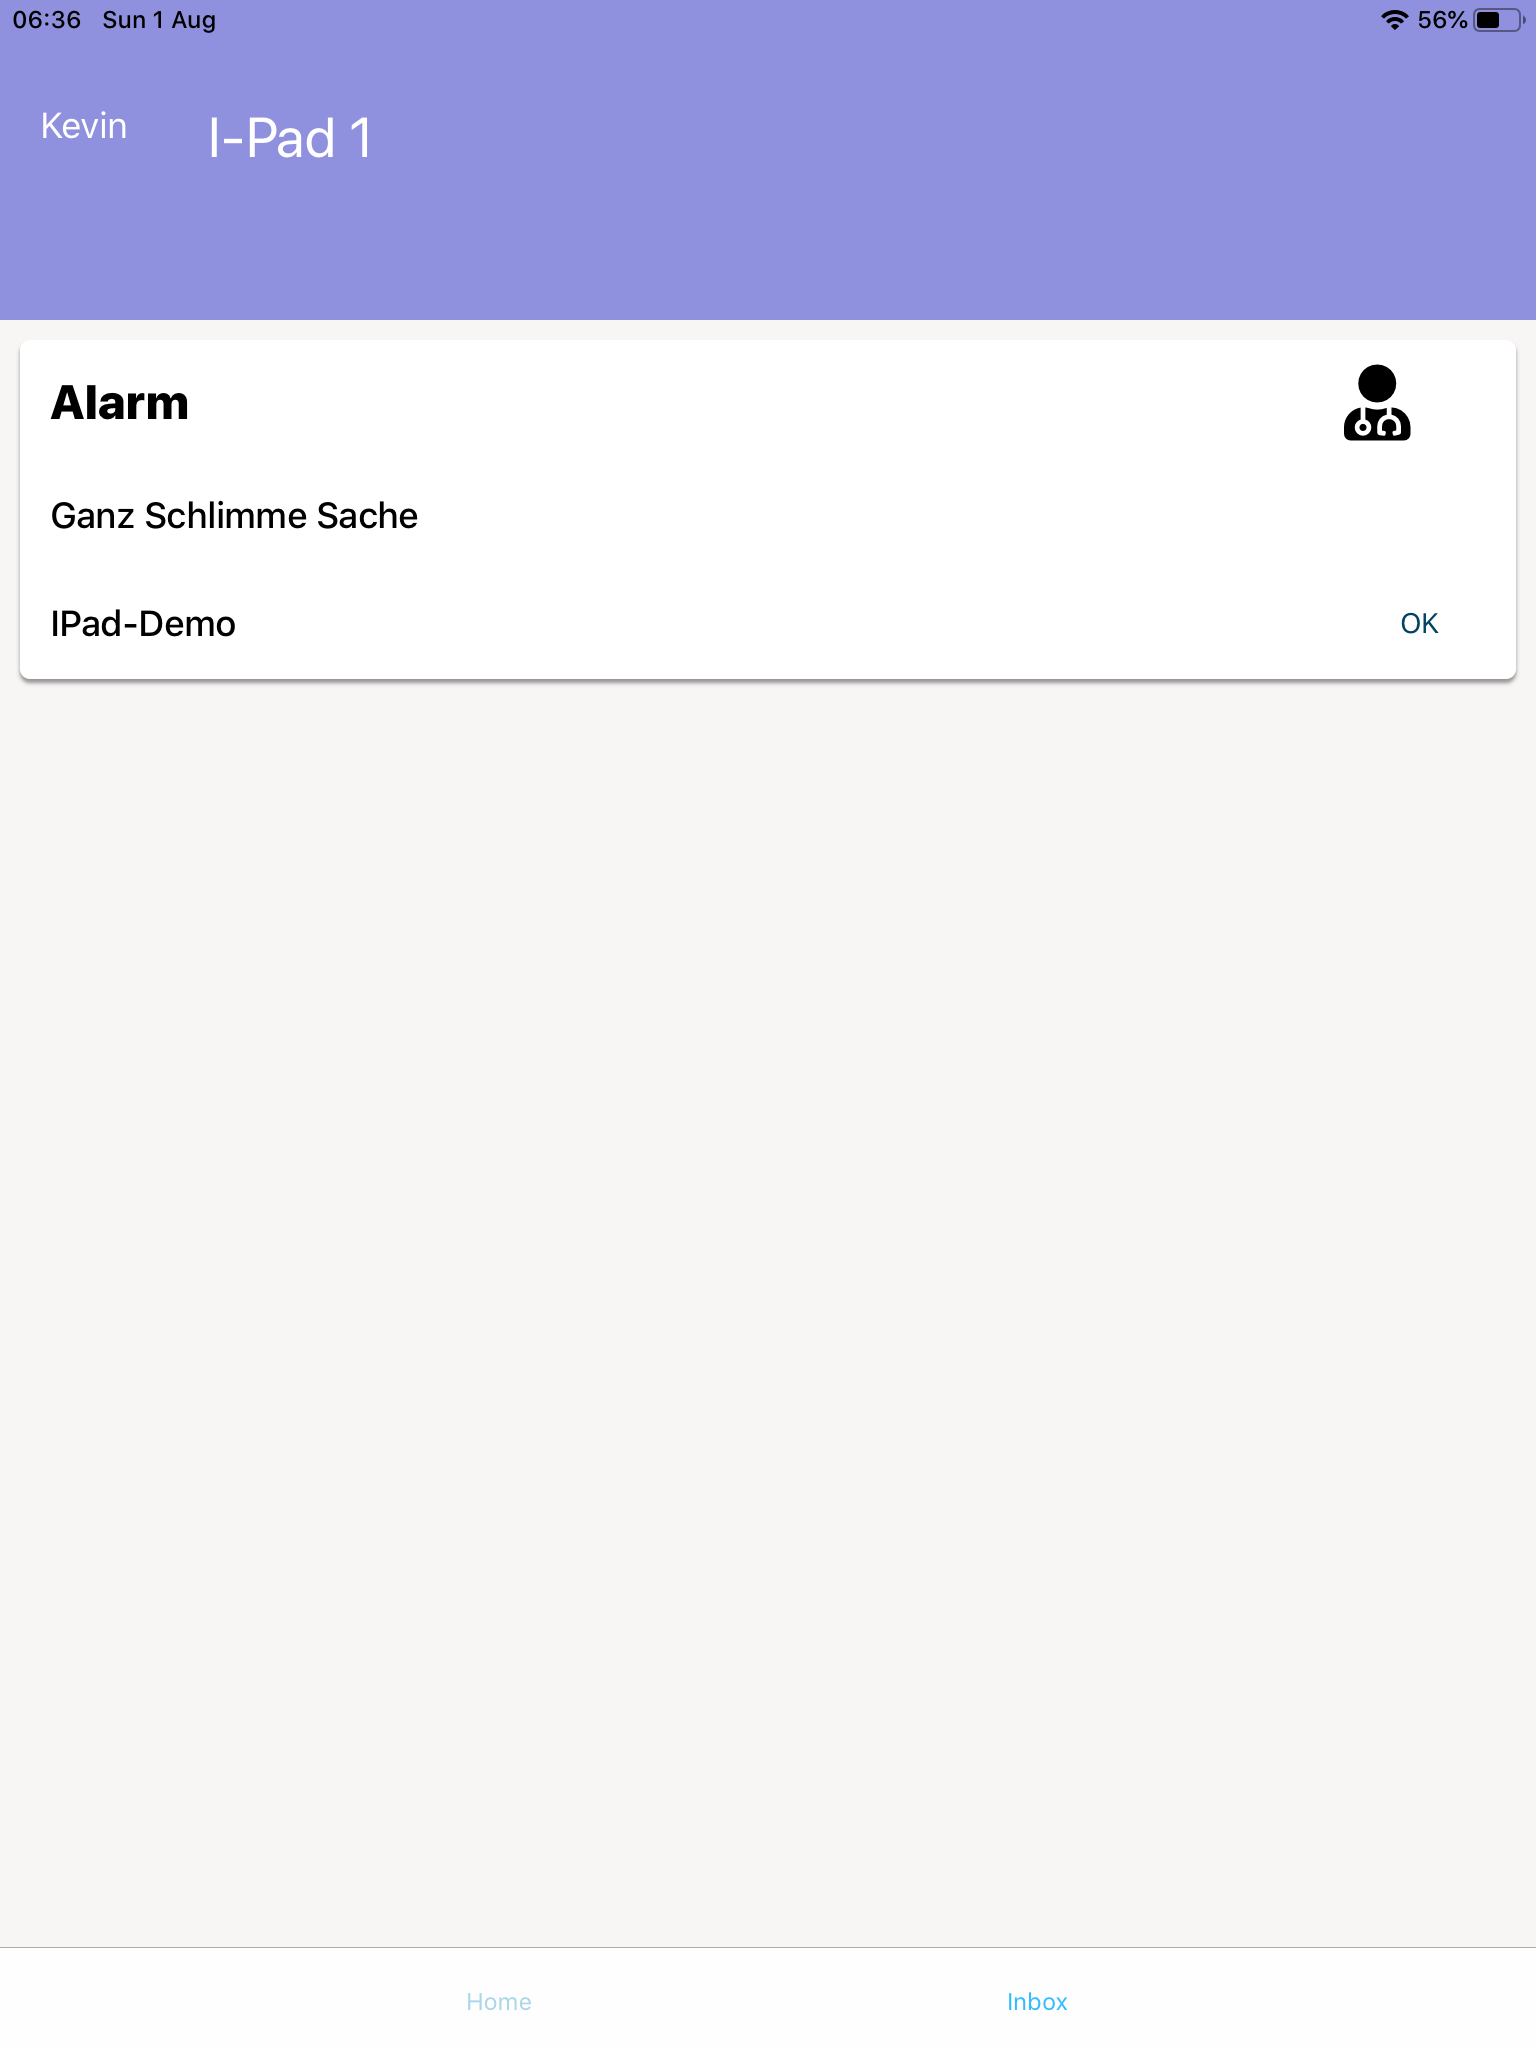
\includegraphics[width=\textwidth]{graphics/screenshots/mobileclient/screenshots-inbox}
        \caption{Inbox}
    \end{minipage}
    \hfill
    \begin{minipage}[b]{0.4\textwidth}
        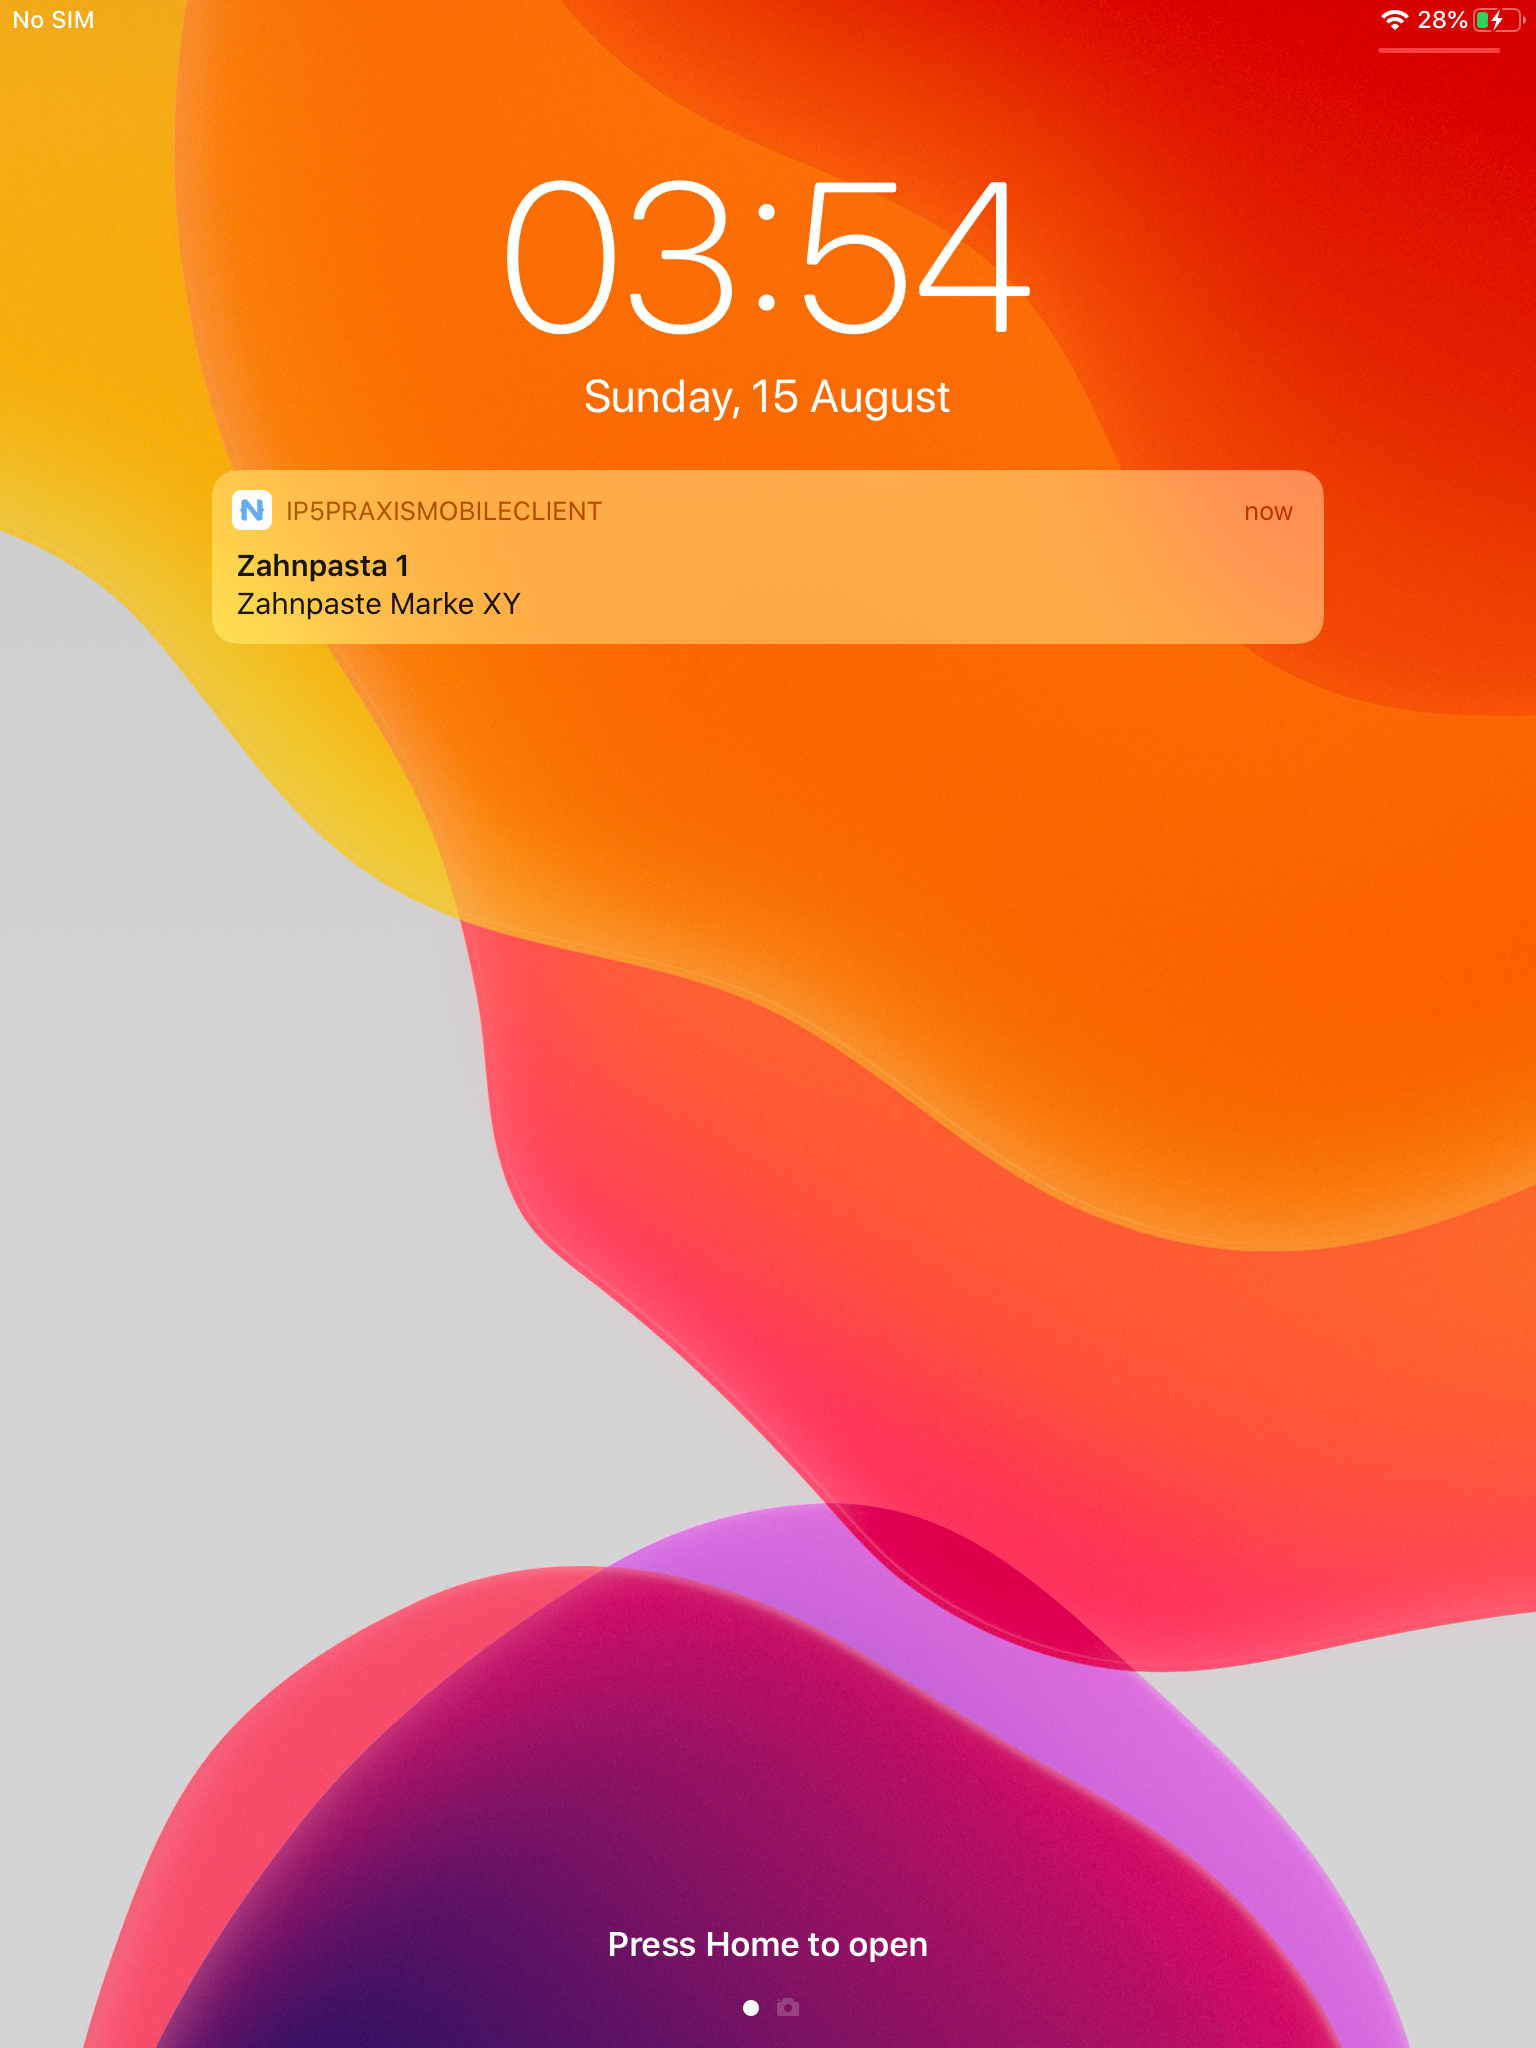
\includegraphics[width=\textwidth]{graphics/screenshots/mobileclient/screenshot-push}
        \caption{Push Benachrichtigung}
    \end{minipage}
    \label{fig:MobileClient-Screens3}
\end{figure}

\clearpage


        
\subsection{Cloud Service}\label{subsec:cloud-service}

\subsubsection{Architektur}

Es gibt deren Domänen 2. Configuration und Notification.

So quasi als ob man 2 Microservices haben kann. Aber wär halt doof das für den stand jetzt schon so zu trennen, deshalb vorerst mal erst ein einzelnes.

\clearpage

\subsubsection{Domänenmodell}


Für die beiden Domänen gibt es natürlich auch so n paar Diagramme. Die gibts jetzt hier:


\subsubsection*{Domäne Configuration}

\begin{figure}[h]
    \centering
    \begin{minipage}[b]{1.0\textwidth}
        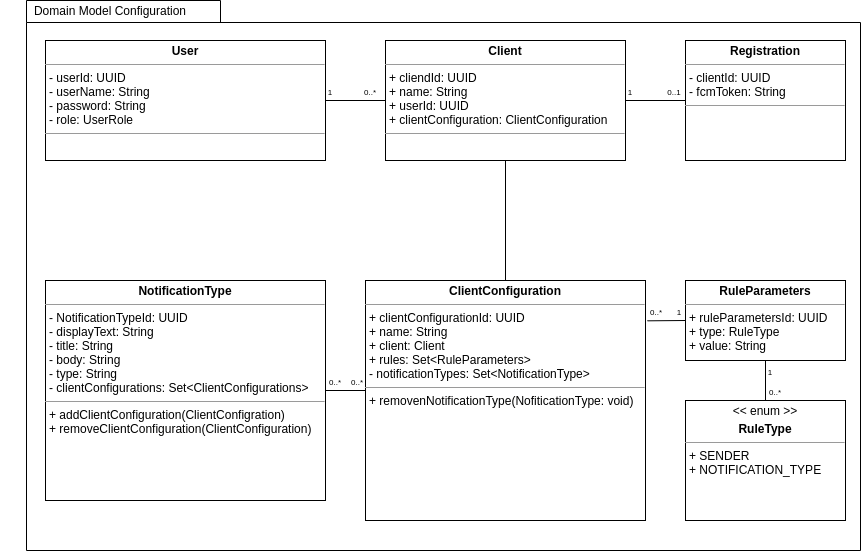
\includegraphics[width=\textwidth]{graphics/Class_Configuration_Domain}
        \caption{Domänenmodell Configuration}
    \end{minipage}
\end{figure}

\clearpage
\subsubsection*{Domäne Notification}

\begin{figure}[h]
    \centering
    \begin{minipage}[b]{1.0\textwidth}
        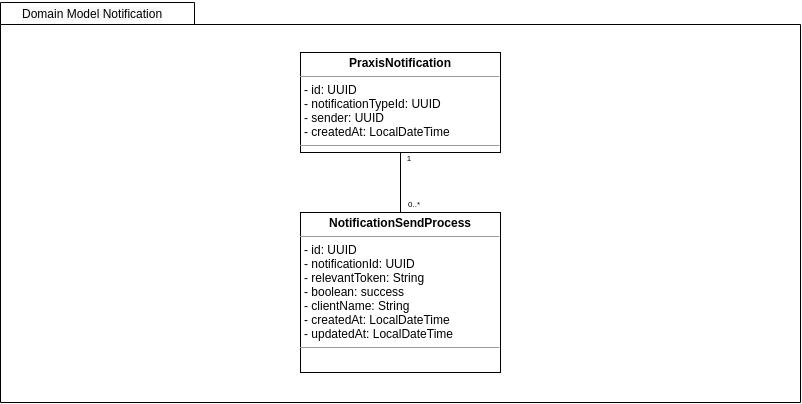
\includegraphics[width=\textwidth]{graphics/Class_Notification_Domain}
        \caption{Domänenmodell Notification}
    \end{minipage}
\end{figure}

\clearpage
\subsubsection*{Rules Engine}

Strategy Pattern mit Spring is noch nice.

\begin{figure}[h]
    \centering
    \begin{minipage}[b]{1.0\textwidth}
        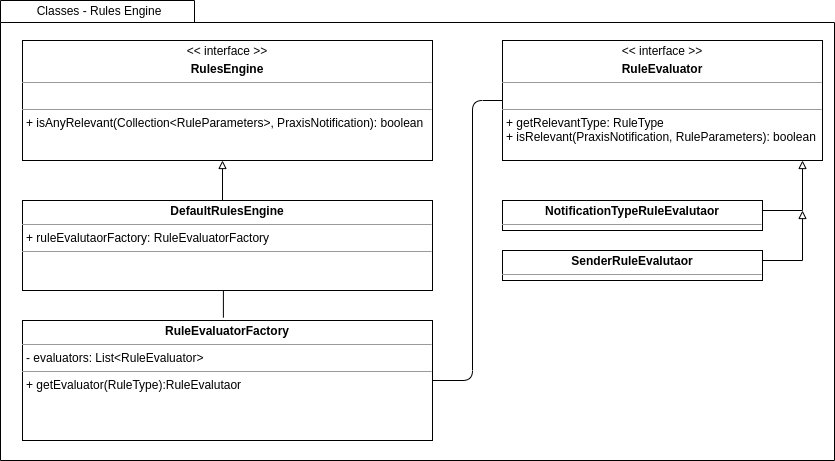
\includegraphics[width=\textwidth]{graphics/Class_Configuration_RulesEngine}
        \caption{Klassendiagramm Rules Engine}
    \end{minipage}
\end{figure}



\clearpage
\subsubsection{API}

S gibt da n paar controller und die brauchen ein paar services.

\clearpage
\subsubsection{Laufzeitmodell}

\clearpage

        \subsubsection{Admin UI}

Das Admin UI bietet Praxisverantwortlichen die Möglichkeit die Konfiguration des Praxisrufsystems zu verwalten.
Da nur Praxisverantworliche das Admin UI verwenden dürfen, ist die Benutzeroberfläche durch ein Login geschützt.
Die entsprechenden Anmeldeinformationen müssen bei Installation des Cloud Services vom Betreiber manuell konfiguriert werden.\footnote{Siehe Anhang D}

\begin{figure}[h]
    \centering
    \begin{minipage}[b]{0.4\textwidth}
        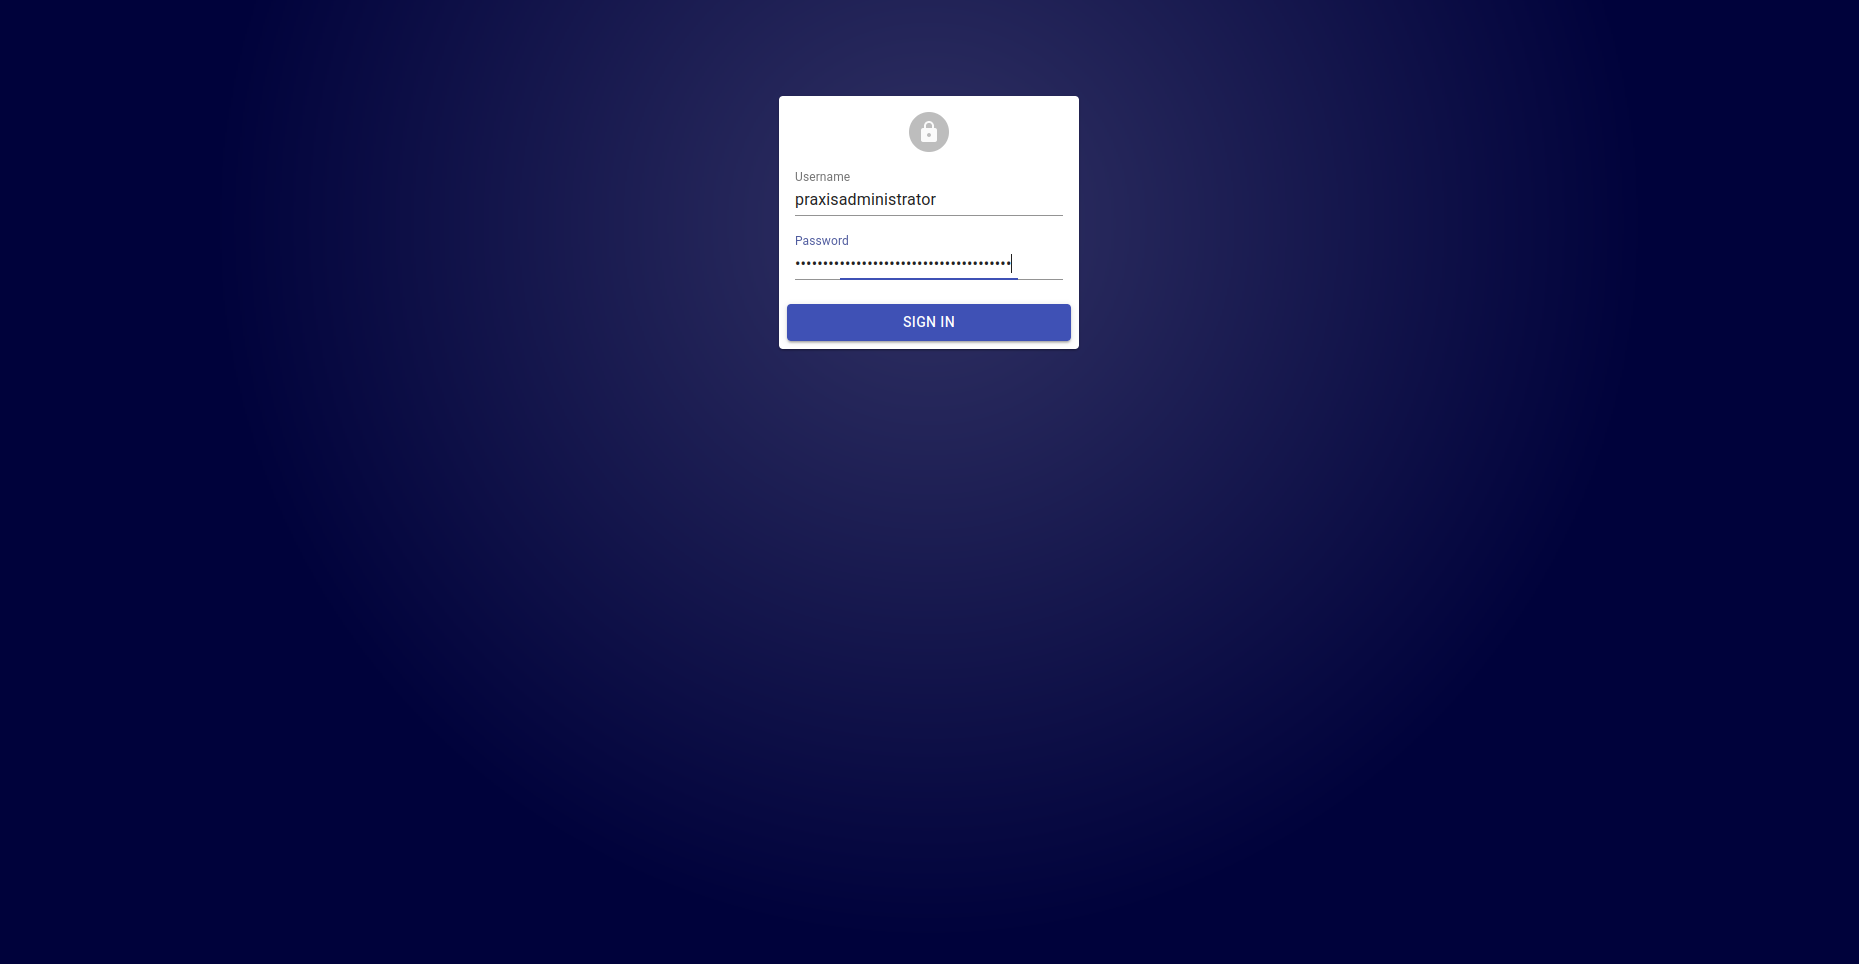
\includegraphics[width=\textwidth]{graphics/screenshots/adminui/login}
        \caption{Login}
    \end{minipage}
    \hfill
    \begin{minipage}[b]{0.4\textwidth}
        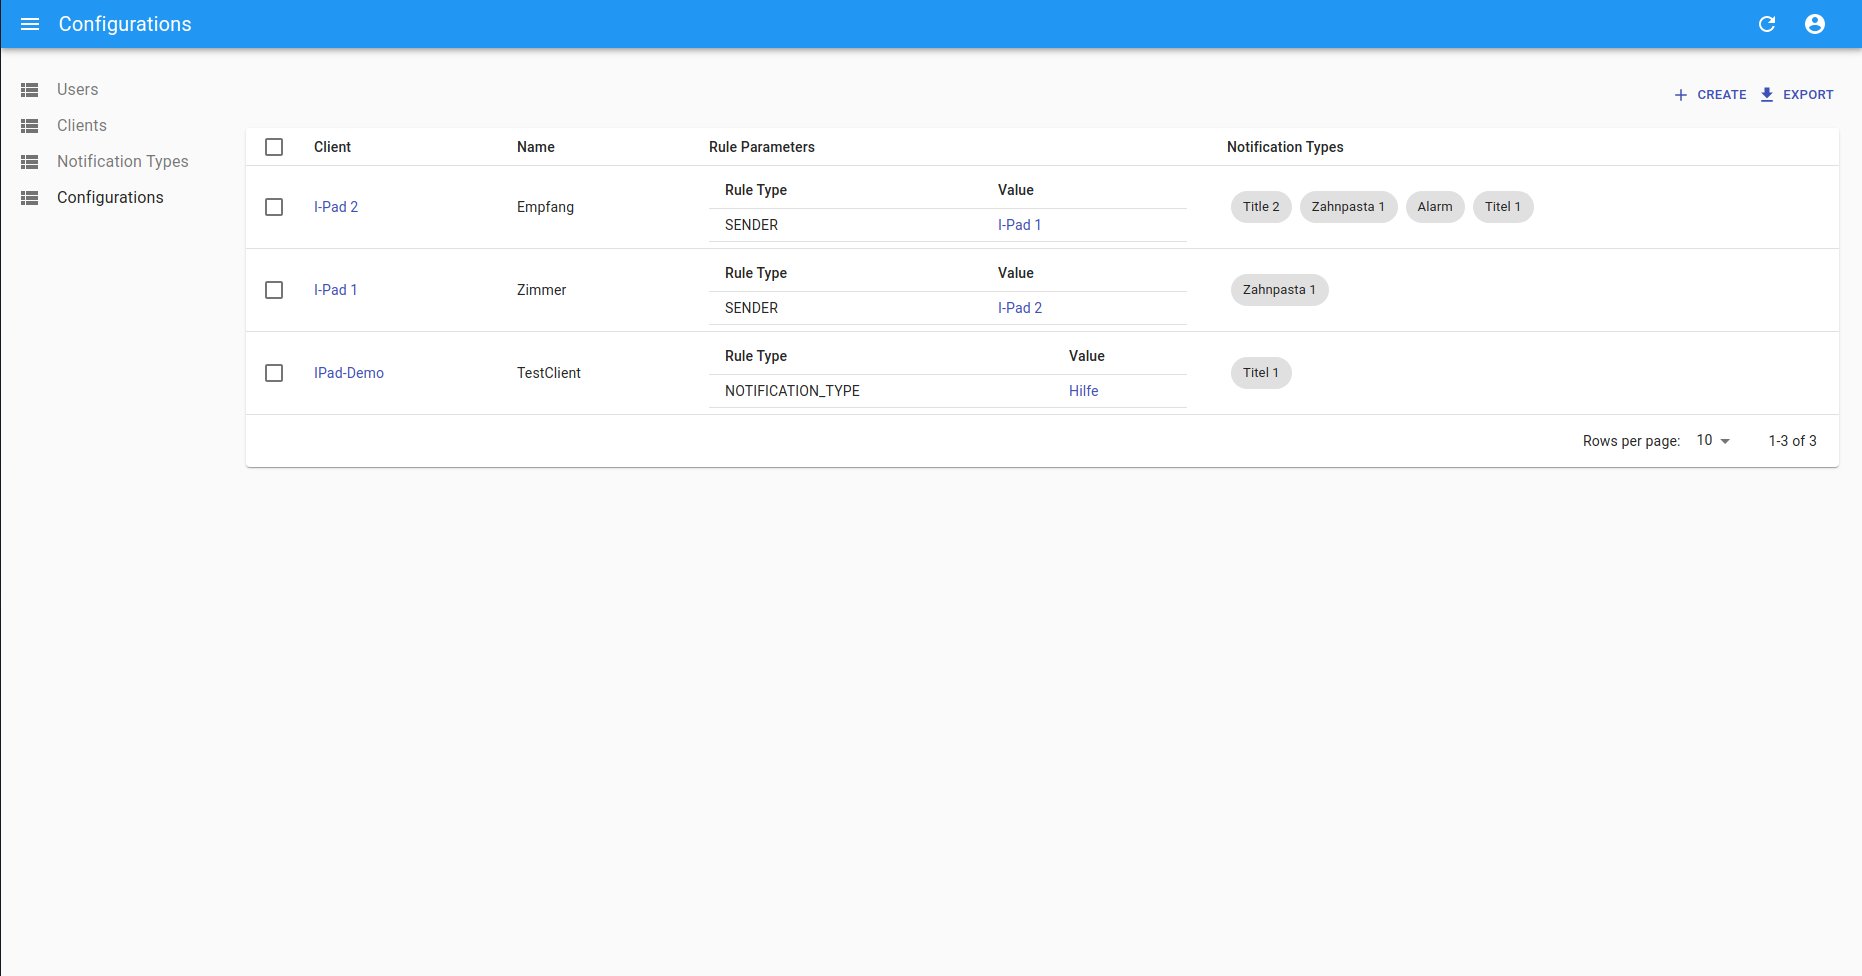
\includegraphics[width=\textwidth]{graphics/screenshots/adminui/configuration-all}
        \caption{Configuration Overview}
    \end{minipage}
    \label{fig:AdminUI-Screens1}
\end{figure}

Das Admin UI beinhaltet vier Bereiche.
Der Bereich Users dient dazu Benutzer zu erstellen, welche sich als Benutzer am Mobile Client anmelden können.
Unter dem Bereich Clients können Geräte verwaltet werden.
Jeder Client ist eindeutig einem Benutzer zugewiesen.
Im Bereich Notification Types können Benachrichtigungen verwaltet werden.
Hier wird konfiguriert, welchen Text der Button für diese Benachrichtigungen im Mobile Client hat und welchen Inhalt die Benachrichtigung hat, wenn sie versendet wird.
Unter dem Bereich Configurations wird die zentrale Konfiguration eines Clients verwaltet.
Jede Konfiguration wird genau einem Client zugewiesen.
Die Konfiguration beinhaltet eine Liste von Notification Types, welche auf dem zugewiesenen Mobile Client als Versenden Button angezeigt werden.
Weiter definiert die Konfiguration eine Liste von Regel Parametern, welche bestimmen, welche Benachrichtigungen dem zugewiesenen Client weitergeleitet werden.

\begin{figure}[h]
    \centering
    \begin{minipage}[b]{0.4\textwidth}
        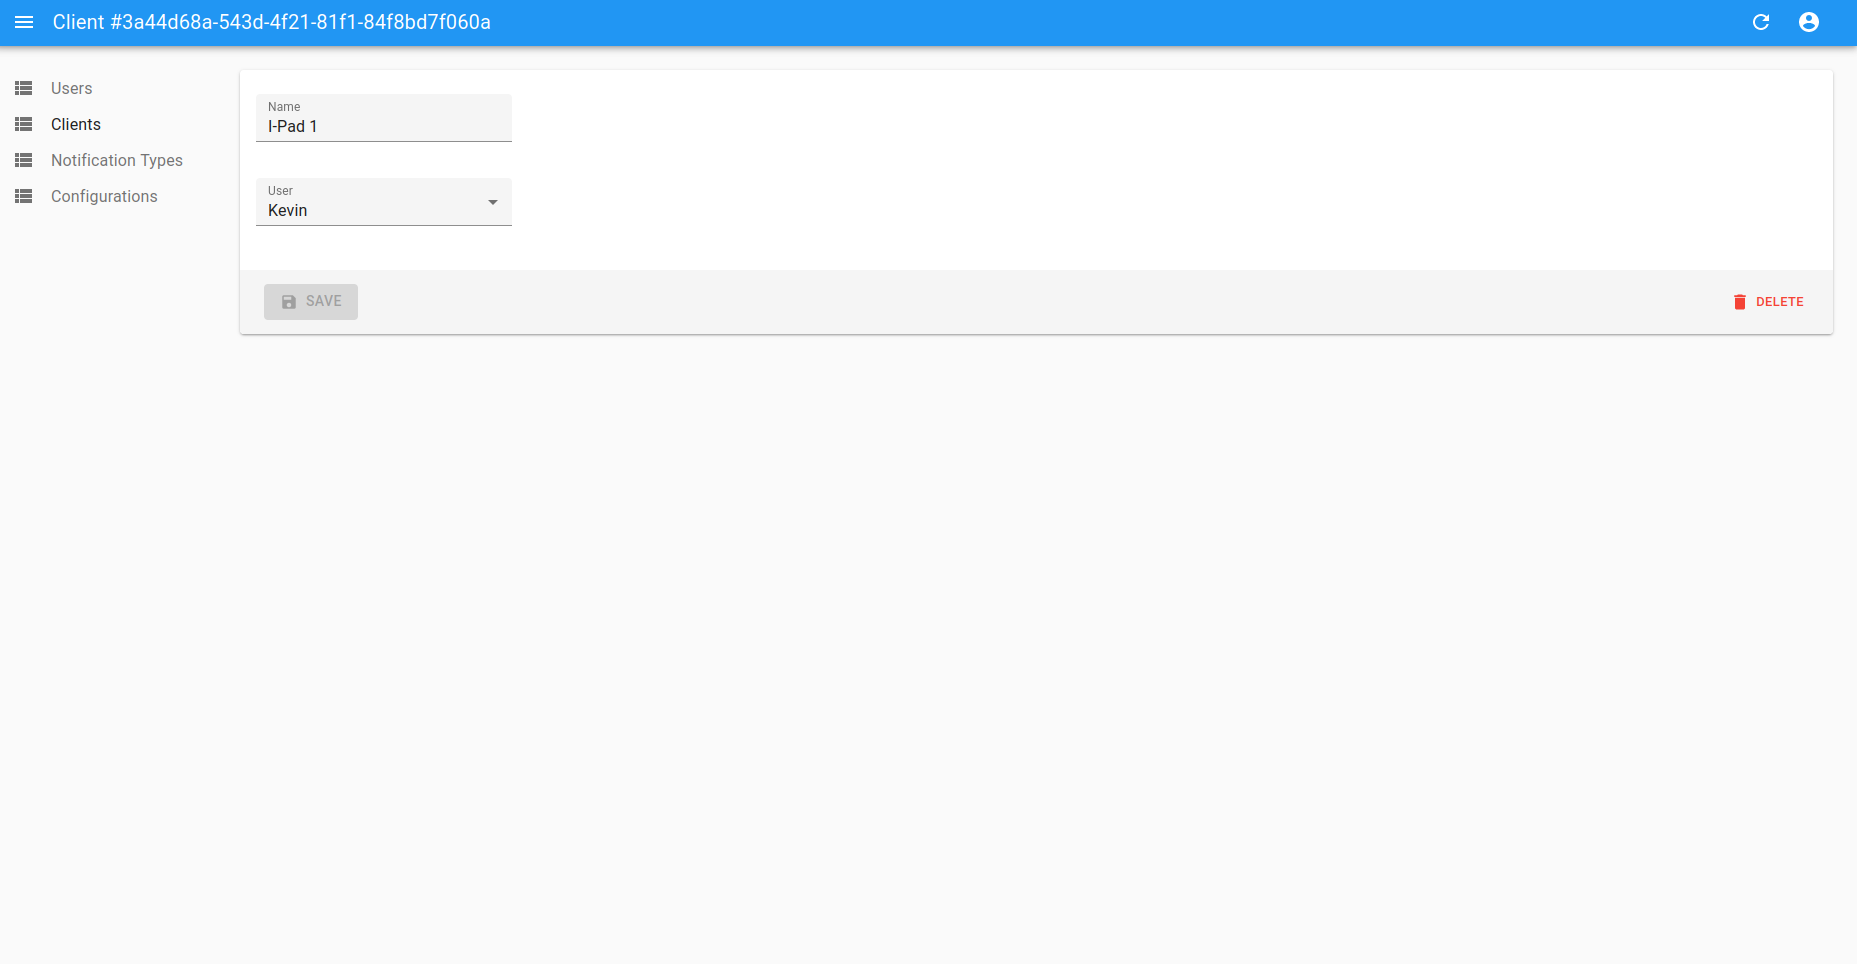
\includegraphics[width=\textwidth]{graphics/screenshots/adminui/configuration}
        \caption{Login}
    \end{minipage}
    \hfill
    \begin{minipage}[b]{0.4\textwidth}
        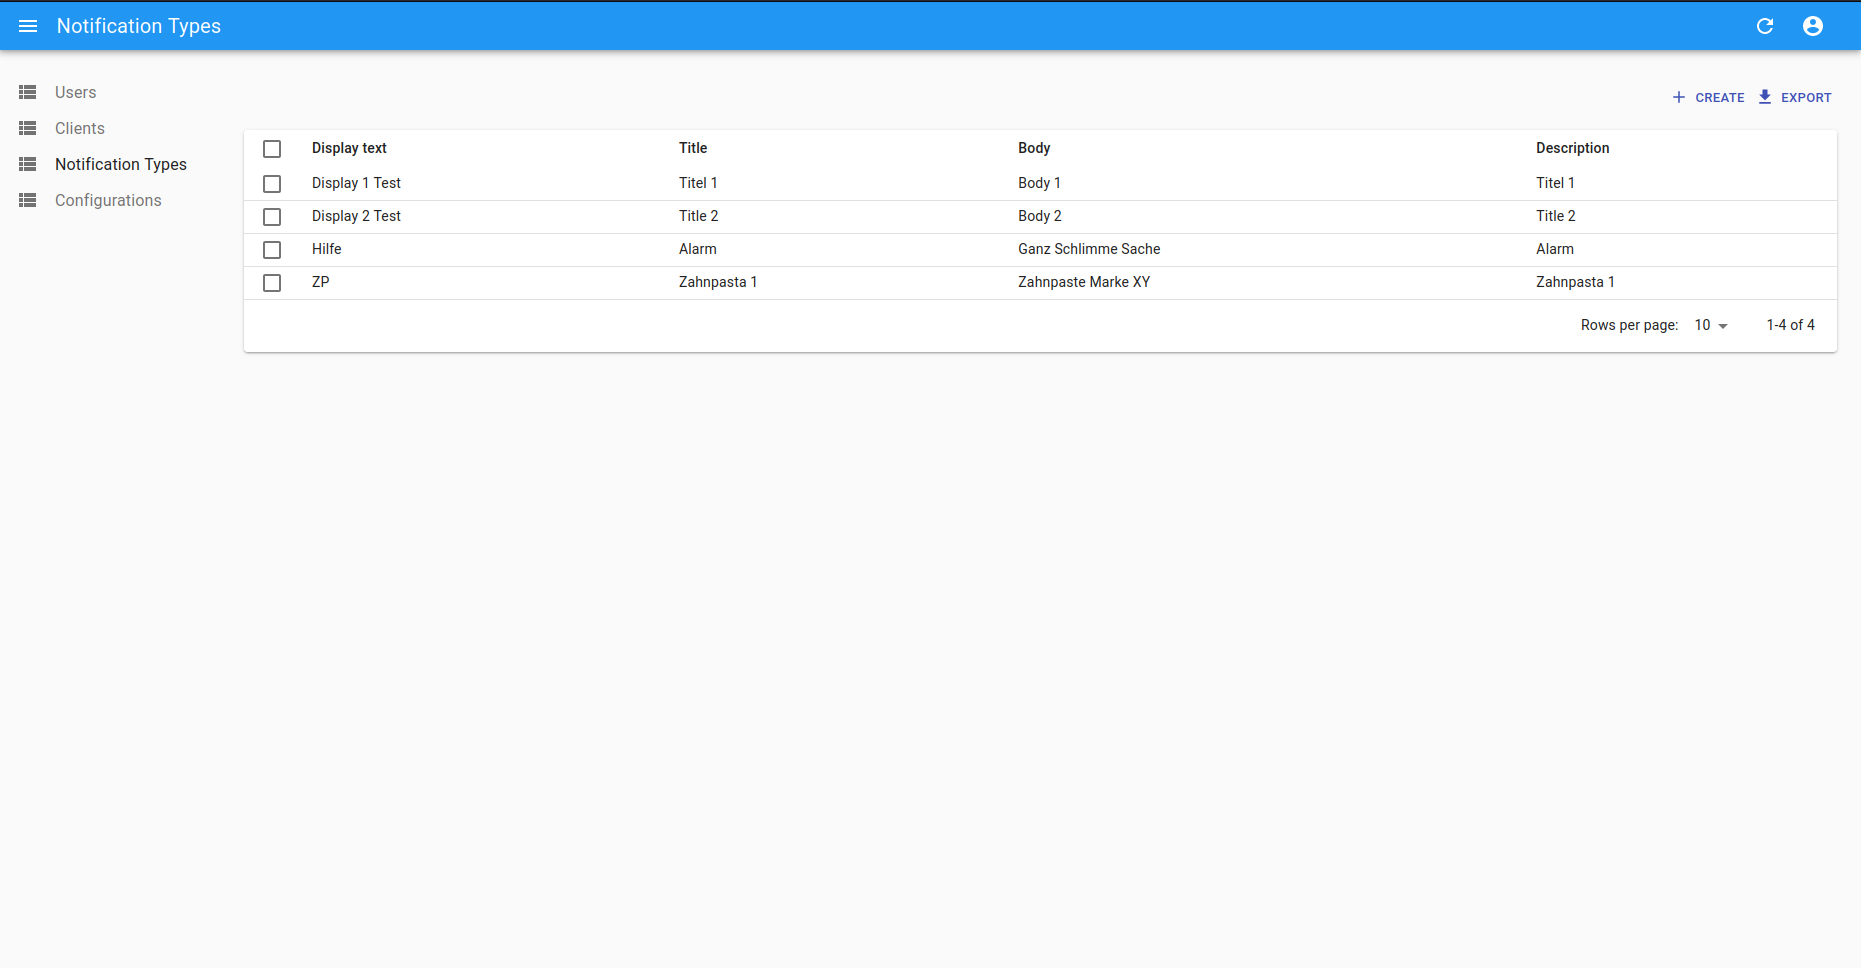
\includegraphics[width=\textwidth]{graphics/screenshots/adminui/notification-type}
        \caption{Configuration Overview}
    \end{minipage}
    \label{fig:AdminUI-Screens2}
\end{figure}

Jeder der Bereiche im Admin UI bietet dem Benutzer die Möglichkeit, den jeweiligen Teil der Konfiguration zu lesen, erstellen, bearbeiten und löschen.
Auf der Startseite jedes Bereiches wird eine Liste mit allen relevanten Einträgen angezeigt.
Mehr Informationen zur Bedienung des Admin UIs befinden sich im Benutzerhandbuch.\footnote{Siehe Anhang C}

\clearpage


    \subsection{Tests}

        \subsubsection*{Benutzertests}

\subsubsection*{Testablauf}

Am 21. Juli 2021 wurden zusammen mit dem Auftraggeber Benutzertests durchgeführt.
Dazu wurde der Mobile Client auf in physisches Ipad installiert.
Zusätzlich wurde eine zweite Mobile Client Instanz auf einem Emulator gestartet.
Der Cloud Service sowie das Admin UI wurden mit Amazon Webservices deployt.
Ein Firebase Messaging Service wurde angebunden.

Für die Benutzertests wurde folgender Ablauf durchgespielt:

\begin{enumerate}
    \item Client 1 im Admin UI anlegen und Benutzer 1 zuweisen.
    \item Client 2 im Admin UI anlegen und Benutzer 1 zuweisen.
    \item Einen neuen Notification Type im Admin UI anlegen
    \item Eine Client Configuration für Client 1 erstellen und darauf den erfassten Notification Type setzen.
    \item Eine Client Configuration für Client 2 erstellen und Regel Parameter erfassen, das alle Benachrichtigungen von Client 1 empfangen werden sollen.
    \item Mobile Client auf Ipad starten
    \item Auf Ipad mit Benutzer 1 anmelden.
    \item Auf Ipad Client 2 auswählen.
    \item Mobile Client auf Emulator starten.
    \item Auf Emulator mit Benutzer 1 anmelden.
    \item Auf Emulator Client 1 auswählen.
    \item Auf Emulator Benachrichtigung auslösen.
\end{enumerate}

Der Test wurde zweimal durchgeführt.
Bei der ersten Durchführung war die Mobile Client Applikation auf dem Empfänger Gerät im Vordergrund geöffnet.
Bei der zweiten Durchführung wurde die Mobile Client Applikation auf dem Empfänger Gerät minimiert.
In beiden Fällen wurde erwartet, dass die Benachrichtigung in der Inbox des Empfängers angezeigt wird.
Im zweiten Fall wurde zusätzlich erwartet, dass eine Push-Benachrichtigung angezeigt wird.

Mehr oder frühere Benutzertests konnten aufgrund der pandemischen Situation nicht durchgeführt werden.

\subsubsection*{Feedback vom Benutzer}

Aus den Tests mit dem Benutzer sind folgende zusätzliche Anforderungen hervorgegangen:

\begin{itemize}
    \item Wenn Benachrichtigungen eingehen sollte ein Audiosignal ertönen.
    \item Wenn Benachrichtigungen nicht quittiert werden, soll ein Erinnerungston ertönen.
    \item Wenn Benachrichtigungen quittiert werden, soll der Versender darüber informiert werden.
\end{itemize}

Um diesen Wünschen Gerecht zu werden, wurden die Szenarien S07 und S09 hinzugefügt.\footnote{Siehe Anhang E}
Diese Anforderungen konnten im Rahmen des Projektes umgesetzt werden.
Der dritte Wunsch des Kunden, die Quittierung von Benachrichtigungen an den Sender weitergeleitet wird konnte aus zeitlichen Gründen nicht mehr umgesetzt werden.

\clearpage


        \subsubsection*{Testplan}

Aus den vervollständigten Features und Szenarien wurde der finale Testplan für das umgesetzte System definiert.
Alle Szenarien sind detailliert im Anhang E beschrieben.
Jedes Szenario definiert die erwarteten Vorbedingungen, einen Testschritt und die zu verifizierenden Ergebnisse.
Diese Szenarien dienen als Grundlage für den Testplan, wobei jedes Szenario einen Testfall darstellt.

Folgendes Protokoll zeigt den Stand der letzten Ausführung der Tests am 19.08.2021:

\begin{table}[h]
    \centering
    \begin{tabular}{|l|p{11cm}|c|c|}
        \hline
        \textbf{Szenario} & \textbf{Beschreibung}                                                                                                                                  & \textbf{Resultat} \\
        \hline
        S01         & Benachrichtigung versenden - Empfänger konfiguriert   & +\\
        \hline
        S02         & Benachrichtigung versenden - kein Empfänger & +\\
        \hline
        S03         & Benachrichtigung empfangen.  & +\\
        \hline
        S04         & Fehler beim Versenden anzeigen.  & +\\
        \hline
        S05         & Wiederholen im Fehlerfall bestätigen.  & +\\
        \hline
        S06         & Wiederholen im Fehlerfall abbrechen.  & +\\
        \hline
        S07         & Audiosignal bei Benachrichtigung.   & +\\
        \hline
        S08         & Push Benachrichtigung im Hintergrund.  & +\\
        \hline
        S09         & Erinnerungston für nicht Quittierte Benachrichtigungen.   & +\\
        \hline
        S10         & Start Mobile Client - nicht angemeldet   & +\\
        \hline
        S11         & Start Mobile Client  - angemeldet & +\\
        \hline
        S12         & Anmelden mit korrekten Daten.   & +\\
        \hline
        S13         & Anmeldung mit ungültigen Daten.   & +\\
        \hline
        S14         & Konfiguration Wählen   & +\\
        \hline
        S15         & Abmelden.   & +\\
        \hline
        S16         & Admin UI - Anmeldung mit korrekten Daten   & +\\
        \hline
        S17         & Admin UI - Anmeldung mit ungültigen Daten   & +\\
        \hline
        S18         & Admin UI - Konfiguration Verwalten   & +\\
        \hline
    \end{tabular}\label{tab:testplan}
\end{table}
\clearpage


    \subsection{Fazit}

In diesem Kapitel werden die zentralen Herausforderungen während der Projektarbeit und die Schlussfolgerungen die wir daraus ziehen beschrieben.

Die grösste Herausforderung im Projekt waren Entwicklung und Konzept des Mobile Clients mit einer geteilten Codebasis für iOS und Android.
Die Recherchen und Tests in diesem Bereich haben deutlich mehr Zeit in Anspruch genommen, als ursprünglich geplant.
Mit der gewählten Technologie Native Script konnten die Anforderungen and den Mobile Client schlussendlich umgesetzt werden.
Grosse Teile des Mobile Clients konnten für Android und iOS gleichzeitig umgesetzt werden.
An den Stellen wo die Applikation mit dem Betriebssystem interagieren muss, müssen aber Unterschiede gemacht werden und Betriebssystemspezifische Plugins verwendet werden.
Die Dokumentation des Frameworks zeigt, das es eine Vielzahl von Plugins gibt und somit fast alle Funktionen die eine native Applikation bietet auch mit Native Script umgesetzt werden können.
Während der Entwicklung mussten wir jedoch feststellen, dass diese Anbindungen in der Praxis oft nicht wie erwartet funktionieren.
Entweder, weil Plugins unvollständig dokumentiert und implementiert sind oder, weil ein Plugin nur mit einer spezifischen Version von Nativescript oder iOS funktioniert.
Dies zeigt, dass eine geteilte Codebasis für mehrere Plattformen Zeit bei der Entwicklung und Wartung sparen kann.
Sie bringt aber den Nachteil, dass die Applikation komplizierter wird, weil trotzdem oft zwischen den unterstützten Betriebssystemen unterschieden werden muss.
Weiter erschwert es die Verwendung von Betriebssystemfunktionen und Gerätehardware, da diese für alle Betriebssystem abstrahiert werden müssen.
Schlussendlich bringt dies eine zusätzliche Schicht in die Architektur die bei Änderungen am Betriebssystem und am Framework Änderungen benötigt.
Dies erhöht den Wartungsaufwand deutlich und kann langfristig Probleme für die Kompatibilität mit dem Betriebssystem verursachen.

Wir schliessen daraus, dass eine geteilte Basis vor allem bei Applikationen die keine oder nur wenig Interaktion mit dem Betriebssystem benötigen, einen Vorteil bietet.
Sobald aber kritische Teile der Applikation mit betriebssystemnahen Funktionen zusammenhängen, empfehlen wir mehrere native Applikationen zu entwickeln.
Der Nachteil, dass Funktionen doppelt implementiert werden müssen wird durch bessere Zukunftssicherheit und einfachere Anbindung an das Betriebssystem aufgehoben.

Eine weitere Herausforderung war das Konzept für den Cloud Service zu erstellen.
Dieser musste ein konfigurierbares Subscription System bieten über den die Mobile Clients Benachrichtigungen versenden und empfangen können.
Bedingung dafür war dass, individuell Regeln konfiguriert werden können die an unterschiedlichen Bedingungen prüfen, welche Benachrichtigungen für welche Clients relevant sind.
Dabei ist es wichtig, dass das Konzept es ermöglicht in Zukunft mit geringem Aufwand weitere Regeln zu implementieren.
Neben dem Regelwerk für Benachrichtigungen war auch die Erweiterbarkeit und Skalierbarkeit des Cloud Services als Ganzes eine Herausforderung.
Anfänglich sind wir davon ausgegangen, dass sich der Cloud Service als einfache Applikation mit einem Endpunkt für Konfiguration und einem Endpunkt für Benachrichtigungen umsetzen lässt.
Die Entwicklungs- und Konzeptphase haben aber gezeigt, dass es auch innerhalb der Domänen eine saubere Aufteilung braucht.
Dementsprechend musste die API aufgeteilt werden, um die Weiterentwicklung und Wartbarkeit des Projektes zu gewähren.
Das Aufsetzten der Entwicklungs- und Betriebsstruktur mit Amazon Webservices hat ebenfalls deutlich mehr Zeit als geplant in Anspruch genommen.
Diese Projektarbeit hat gezeigt, das AWS alle nötigen Mittel bietet, um ein cloudbasiertes Praxisrufsystem zu betreiben.
Damit dies effizient umgesetzt werden kann ist es aber essenziell, ein Konzept zu erstellen, welches die benötigten Dienste und Konfigurationen beschreibt.
Das Installationshandbuch im Anhang kann als Vorlage für ein solches Konzept dienen\footnote{Siehe Anhang D}.

Wir haben gelernt, dass es zentral ist alle Konzepte bei Projektstart zu erstellen.
Die Konzepte müssen dabei nicht von Anfang an ausgereift sein.
Sie dienen aber als Startpunkt und Orientierungshilfe im Projekt.
Dabei ist es wichtig, dass auch Betriebsinfrastruktur, Skalierbarkait und Erweiterbarkeit von Anfang an bedacht werden.

Die letzte Herausforderung, die hier erwähnt werden soll, betrifft das Erarbeiten der Anforderungen.
Die Anforderungen und Prioritäten laufend mit dem Auftraggeber zu besprechen hat für die Projektarbeit immer klare nächste Ziele gegeben.
Da nicht alle Anforderungen bei Projektanfang vollständig definiert wurden, war es teilweise schwer den aktuellen Stand des Projektes einzuordnen.

Für weitere Projekte in diesem Rahmen empfehlen wir, alle relevanten Anforderungen bei Projektstart so detailliert wie möglich zu erarbeiten.
Diese Anforderungen können im Projektverlauf regelmässig besprochen, priorisiert und wenn nötig angepasst werden.
Dadurch ist es einfacher den Fortschritt des Projekts zu evaluieren und trotzdem möglich schnell auf neue Erkenntnisse zu reagieren.

\clearpage


    \section {Schluss}

Im Rahmen dieser Projektarbeit konnte ein cloudbasiertes Praxisrufsystem umgesetzt werden.
Das umgesetzte System besteht aus einer Mobilen Applikation für iOS und Android, einem Cloud Service und einer Web-Applikation.
Mit Firebase Messaging wurde ein externer Messaging Service angebunden, der es Erlaubt
Zudem wurde eine Entwicklungs- und Betriebsinfrastruktur mit Amazon Webservices aufgebaut, welche es erlaubt den Cloud Service und die Web-Applikation zu betreiben.

Das umgesetzte Praxisrufsystem ermöglicht es Benachrichtigungen über eine Mobile Applikation zu versenden.
Als Endgeräte können dafür IPads oder Android Tablets verwendet und empfangen werden.
Der Mobile Client ermöglicht es dabei Benachrichtigungen auch zu empfangen, wenn die Applikation im Hintergrund läuft und sammelt alle Benachrichtigungen in einer Inbox.
Welche Benachrichtigungen versendet werden können, kann über eine Web-Applikation pro Gerät konfiguriert werden.
Weiter können über die Web-Applikation Regeln definiert werden, welche Benachrichtigungen ein Gerät empfangen soll.
So ist es mit dem Praxisrufsystem möglich vorkonfigurierte Benachrichtigungen an einzelne, mehrere oder alle angebundenen Clients zu versenden.

Das umgesetzte System hat aber durchaus noch Lücken, welche eine produktive Nutzung verhindern könnten.
Das Praxisrufsystem konnte wegen diverser Herausforderungen\footnote{Siehe Kapitel 6} nicht im Umfang wie es in der Aufgabenstellung beschrieben wurde umgesetzt werden.
Die Anforderungen Benachrichtigungen, mit einer Text-To-Speech-Funktion auszugeben und eine Gegensprechanlage für Direkt- und Gruppengespräche wurden weder als Konzept noch in der Praxis umgesetzt.
Dementsprechend bietet das umgesetzte Praxisrufsystem nicht in allen Fällen den Funktionsumfang, der für eine produktive Nutzung nötig wäre.

Werden die Funktionen Text-To-Speech und Gegensprechanlage nicht benötigt, könnte das implementierte System grundsätzlich produktiv eingesetzt werden.
Mit dem aktuellen Stand des Systems ist allerdings nur die Konfiguration von einfachen Regeln möglich.
Wenn in einem produktiven System kompliziertere oder zusammengesetzte Regeln zur Vermittlung von Benachrichtigung benötigt werden, ist das Praxisrufsystem noch nicht einsetzbar.
Das System wurde allerdings so konzipiert, dass zusätzliche und kompliziertere Regeln einfach umgesetzt werden können.
Eine Erweiterung des Systems in diesem Punkt wäre deshalb mit verhältnissmässig kleinem Aufwand möglich.

Die grösste Gefahr für die produktive Nutzung des Systems ist allerdings die umgesetzte mobile Applikation.
Die Technologie mit der die Applikation umgesetzt wurde ermöglicht es, eine Codebasis für Android und iOS Geräte zu teilen.
Dies ermöglicht in einigen Bereichen schnellere Entwicklung und einfachere Wartung.
Es erschwert allerdings die Anbindung von Betriebssystemfunktionen und Zugriff auf Gerätehardeware wie es für eine Gegensprechanlage und Text-To-Speech Funktionen nötig wäre.

Insgesamt sind wir zufrieden mit den Konzepten und Ergebnissen, die aus dieser Arbeit hervorgegangen sind.
Wir sind überzeugt mit dem Konzept für die Registrierung von Mobile Clients und dem Regelwerk für Benachrichtigungen eine erweiterbare, skalierbare Grundlage geschaffen zu haben.
Das umgesetzte Rufsystem bietet eine solide Grundlage um ein konkurrenzfähiges, modernes Praxisrufsystem zu entwickeln, welches alle nötigen Anforderungen für den produktiven Einsatz abdeckt.



%%---APPENDIX----------------------------------------------------------------------------
    \renewcommand\refname{Literaturverzeichnis}
\addcontentsline{toc}{section}{Literaturverzeichnis}
\printbibliography
\cleardoublepage
\listoffigures

\appendix

\section{Aufgabenstellung}\label{sec:aufgabenstellung}
\begin{figure}[h]
    \centering
    \begin{minipage}[b]{0.8\textwidth}
        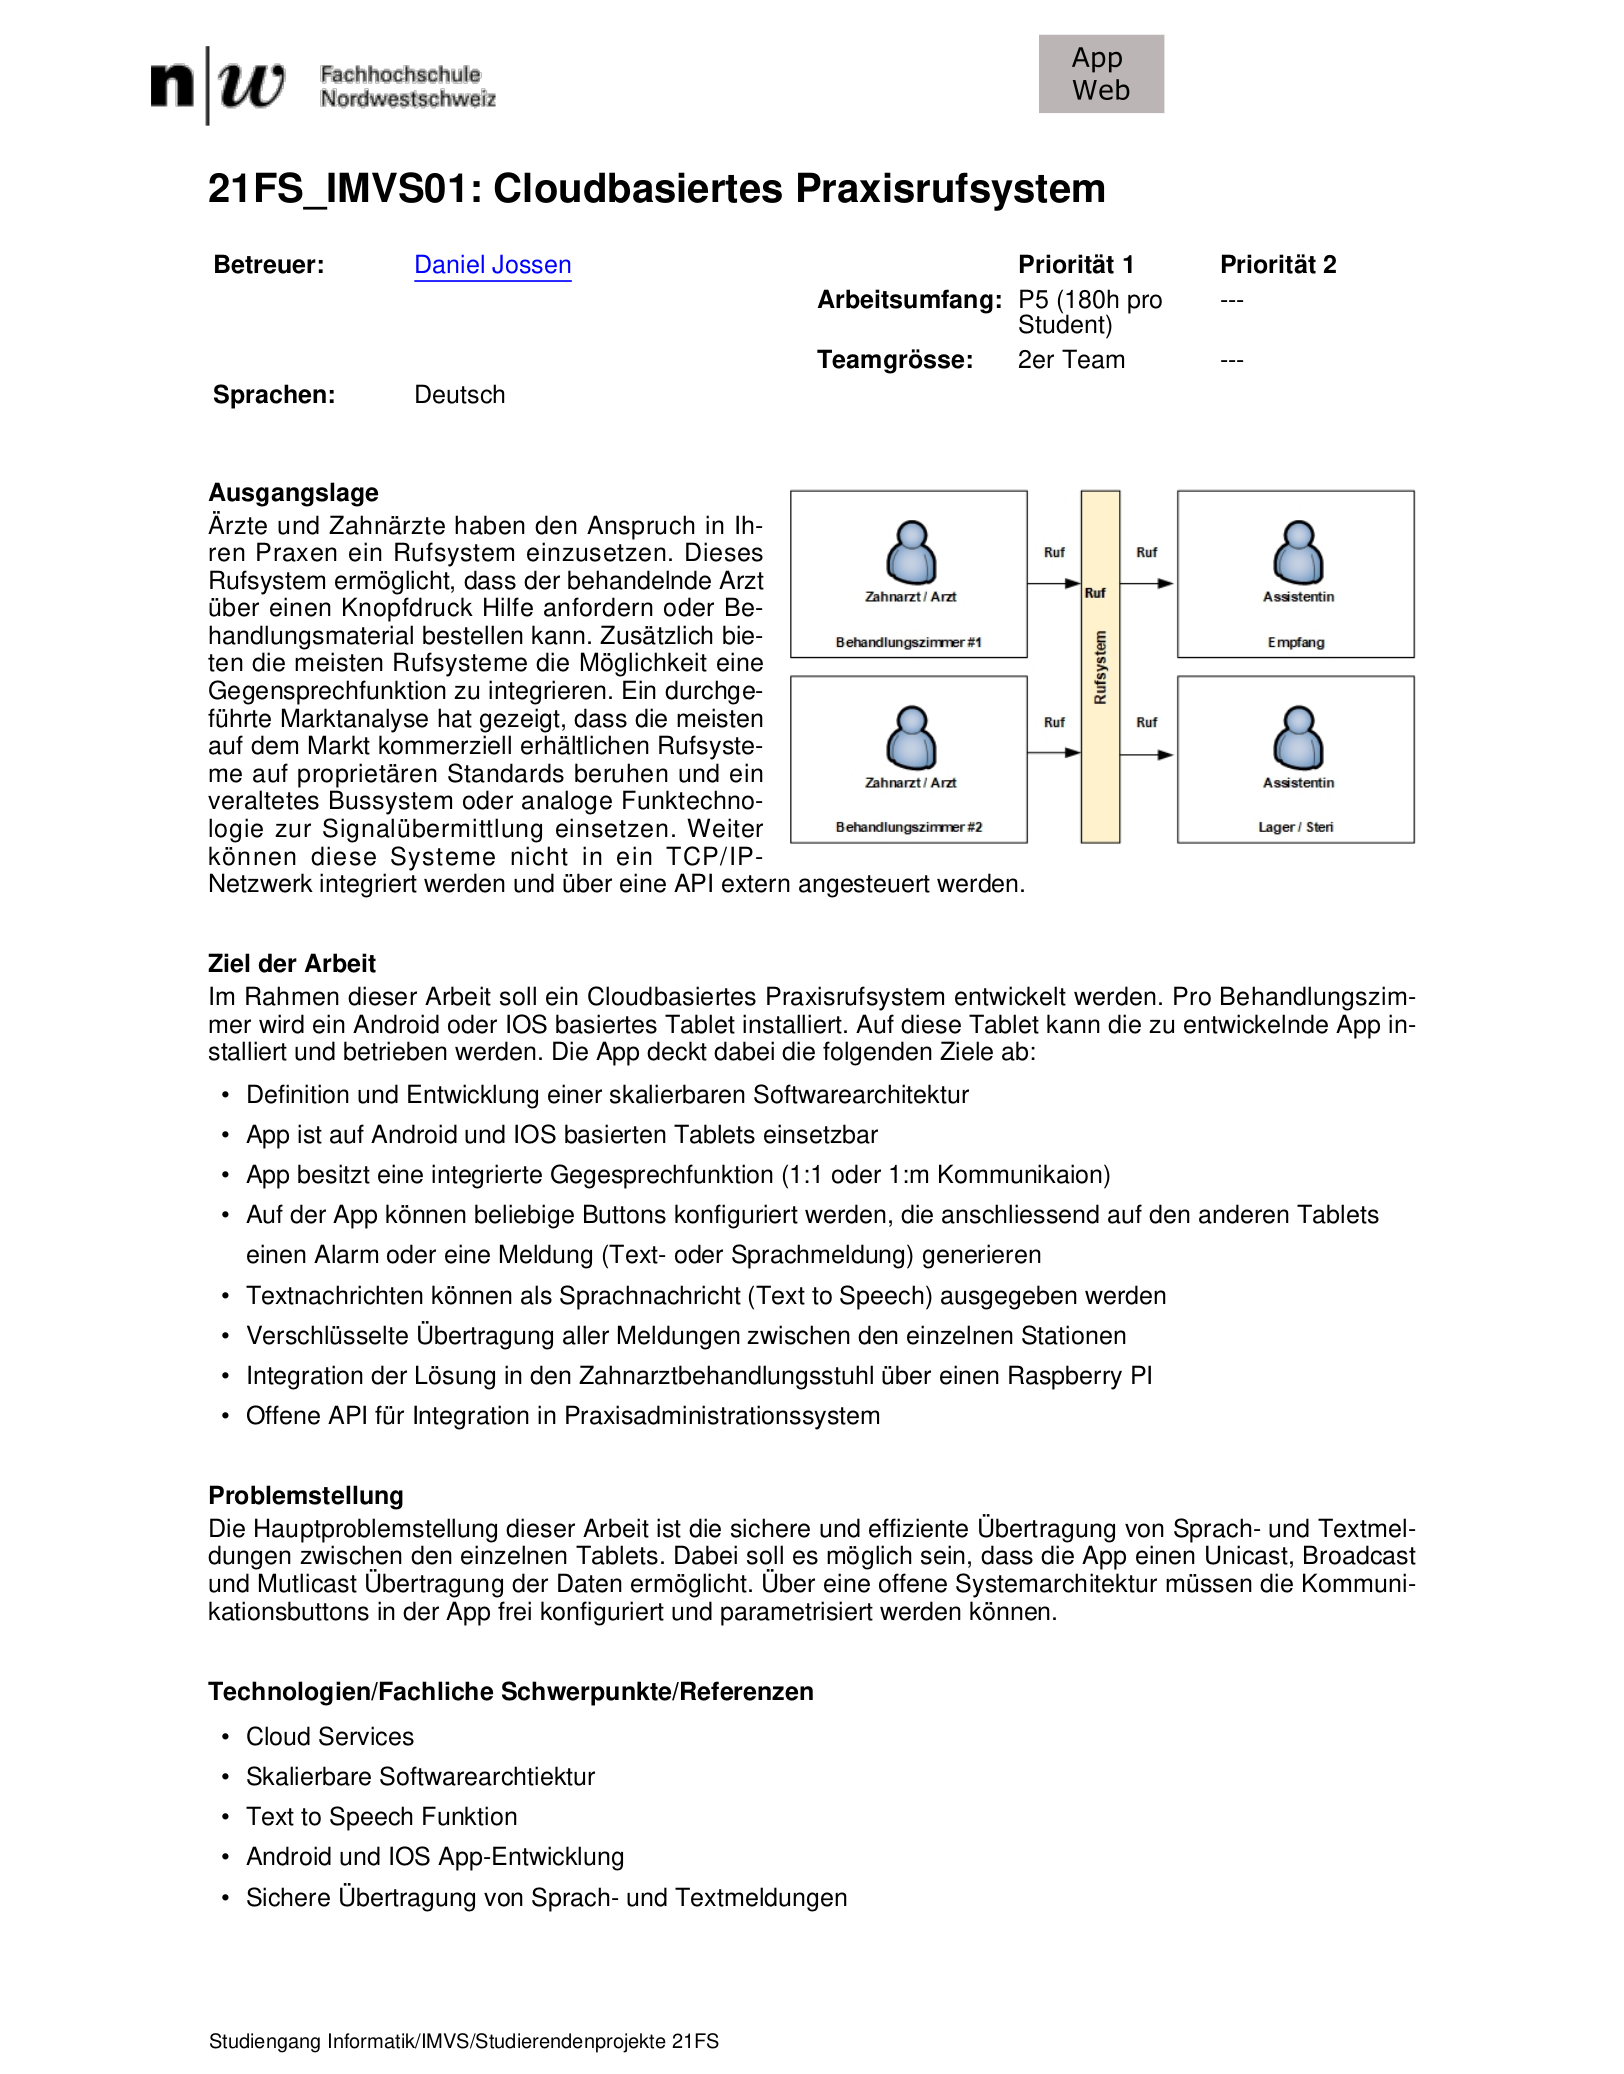
\includegraphics[width=\textwidth]{graphics/aufgabenstellung}
        \caption{Aufgabenstellung}
    \end{minipage}\label{fig:aufgabenstellung}
\end{figure}

\clearpage

\section{Quellcodeverwaltung}\label{sec:quellcodeverwaltung}

Sämtlicher Quellcode der im Rahmen des Projektes entsteht, wurde mit Git verwaltet.
Der Quellcode ist für Berechtigte unter dem Projekt IP5-Cloudbasiertes-Praxisrufsystem auf github.com einsehbar.
(Referenz https://github.com/IP5-Cloudbasiertes-Praxisrufsystem).
Berechtigungen können bei Joshua Villing oder Kevin Zellweger angefordert werden.

\clearpage

\section{Benutzerhandbuch}

\subsubsection*{Mobile Client}

\textbf{Anmeldung und Konfiguration}

\begin{enumerate}
    \item Mobile Client Applikation öffnen
    \item Anmeldedaten eingeben und bestätigen
    \item Gewünschte Konfiguration auswählen
\end{enumerate}

\textbf{Benachrichtigung empfangen}

\begin{enumerate}
    \item In Mobile Client anmelden.
    \item In Navigationsleiste (unten) "Home" auswählen.
    \item Button mit dem gewünschten Titel antippen.
    \item Die Benachrichtigung wird automatisch versendet.
\end{enumerate}

\textbf{Benachrichtigung Auflisten und Quittieren}

\begin{enumerate}
    \item In Mobile Client anmelden.
    \item In Navigationsleiste (unten) "Inbox" auswählen.
    \item In dieser Ansicht sehen Sie alle empfangenen noch nicht quittierten Benachrichtigungen.
    \item Zum Quittieren einer Benachrichtigung kann diese angetippt werden.
\end{enumerate}

\textbf{Abmeldung}

\begin{enumerate}
    \item Mobile Client Applikation öffnen
    \item Auf den Namen in der Kopfleiste tippen
    \item Logout bestätigen
\end{enumerate}

\subsubsection*{Admin UI}

\textbf{Anmeldung}

\begin{enumerate}
    \item Admin UI im Browser öffnen
    \item Anmeldedaten eingeben und bestätigen. Die Anmeldedaten erhalten Sie nach Installation des Systems vom Betreiber.
\end{enumerate}

\textbf{Einträge hinzufügen}
\begin{enumerate}
    \item Melden Sie sich im Admin UI an.
    \item Wählen Sie auf der Linken Seite die Kategorie die Sie verwalten möchten.
    \item Auf dieser Seite können Sie nun Einträge zur gewählten Kategorie verwalten:
    \begin{itemize}
        \item Klicken Sie oben rechts auf die Schaltfläche "Create" um einen neuen Eintrag zu erstellen.
        \item Klicken Sie auf einen Eintrag in der Liste um ihn zu bearbeiten.
        \item Klicken Sie die Checkbox auf der Linken Seite eines Eintrages und dann auf die Schaltfläche "löschen" um einen Eintrag zu löschen.
    \end{itemize}
\end{enumerate}

\textbf{Praxisruf konfigurieren}
\begin{enumerate}
    \item Melden Sie sich im Admin UI an.
    \item Erfassen Sie in der Kategorie "User" pro Praxiszimmer einen Benutzer.
    \item Erfassen Sie in der Kategorie "Client" pro Gerät und Zimmer einen Eintrag und weisen Sie ihn dem Benutzer des entsprechenden Zimmers zu.
    \item Erfassen Sie in der Kategorie "Notification Types" alle Benachrichtigungen die Sie zur Verfügung stellen möchten.
    \item Erfassen Sie in der Kategorie "Configurations" pro Gerät und Zimmer einen Eintrag und weisen es dem entsprechenden Client zu.
    \item Unter Notification Types können die Benachrichtigungen auswählen, die auf diesem Gerät zum Versenden verfügbar sind.
    \item Unter Rule Parameters können Sie Regeln definieren, welche Benachrichtigungen diesem Client zugestellt werden.
\end{enumerate}

\clearpage


\section{Installationsanleitung}

\subsubsection*{Mobile Client}
\textbf{TODO} \\
?? Cloud Service url configuration \\
?? FCM Integration configuration \\

\subsubsection*{Admin UI}

Im Folgenden wird beschrieben wie die Admin UI Applikation mit AWS betrieben werden kann.

\begin{enumerate}
    \item AWS Amplify Service aufsetzen:
    \begin{enumerate}
        \item Amazon Webservice unterstützt die Anbdingun von Github, Gitlab, BitBucket und AWS CodeCommit. Stellen Sie sicher, dass der Quellcode der Admin UI Applikation in einem Git Repository zur Verfügung steht.
        \item Folgen Sie den Schritten in der \href{https://docs.aws.amazon.com/amplify/latest/userguide/getting-started.html}{\textit{offiziellen Anleitung}}.\cite{aws-amplify}
    \end{enumerate}
    \item Verbindung zum Cloud Service konfigurieren:
    \begin{enumerate}
        \item Öffnen sie die AWS Amplify Konsole für die in Schritt 1 erstellte Applikation.
        \item Wählen Sie den Menüpunkt "Environment Variables"
        \item Erstellen Sie eine neue Variable mit dem Namen REACT\_APP\_BACKEND\_BASE\_URI. Setzten Sie als Wert dafür die Domain, unter welcher der Cloud Service erreichbar ist.
    \end{enumerate}
    \item Konfigurieren Sie eine Domain für die Admin UI Applikation.
    \begin{enumerate}
        \item Folgen Sie dazu den Schritten in der \href{https://docs.aws.amazon.com/amplify/latest/userguide/custom-domains.html}{\textit{offiziellen Anleitung}}.\cite{aws-amplify-domain} folgen.
    \end{enumerate}
\end{enumerate}

\subsubsection*{Cloud Service}

Im Folgenden wird beschrieben wie die Cloud Service Applikation mit AWS betrieben werden kann.

\begin{enumerate}
    \item Stellen Sie sicher, dass der Quellcode der Cloud Service Applikation in einem Git Repository bei einem der Anbieter Github, Gitlab, BitBucket oder AWS CodeCommit zur Verfügung steht.
    \item Erstellen Sie einen mit AWS ein Elastic Beanstalk Environment.
    \begin{enumerate}
        \item Folgen Sie dazu der \href{https://docs.aws.amazon.com/elasticbeanstalk/latest/dg/GettingStarted.CreateApp.html}{\textit{offiziellen Anleitung}}\cite{aws-elastic}
        \item Wählen Sie unter Plattform "Java" und die dazugehörigen Standardeinstellungen.
        \item Wählen Sie unter Application Code "Sample Application".
    \end{enumerate}
    \item Erstellen sie mit AWS RDS eine Datenbank für die Cloud Service Applikation
    \begin{enumerate}
        \item In Beanstalk Console
        \item Folgen Sie der \href{https://docs.aws.amazon.com/elasticbeanstalk/latest/dg/using-features.managing.db.html}{\textit{offiziellen Anleitung}}\cite{aws-elastic-rds} um eine Relationale Datenbank an das Beanstalk Environment anzubinden.
        \item Wählen Sie als Datenbank Engine "postgres" in der Version 13.3.
        \item Wenn sie oben genannter Anleitung folgen, ist keine weitere Konfiguration für die Datenbankanbindung im Cloud Service nötig.
        Sollten Sie wählen, die Datenbank auf eine andere Art zu Betreiben müssen in Schritt 4 die Umgebungsvariablen RDS\_HOSTNAME, RDS\_PORT, RDS\_DB\_NAME, RDS\_USERNAME und RDS\_PASSWORD mit den entsprechenden Werten konfiguriert werden.
    \end{enumerate}
    \item Definieren Sie die nötigen Umgebungsvariablen für die Cloud Service Applikation:
    \begin{enumerate}
        \item Folgen Sie der \href{https://docs.aws.amazon.com/elasticbeanstalk/latest/dg/environments-cfg-softwaresettings.html}{\textit{offiziellen Anleitung}}\cite{aws-elastic-env} um die nötigen Umgebungsvariablen zu setzen:
        \item Name: FCM\_CREDENTIALS, Wert: Firebase Credentials mit Base 64 Encoded\footnote{Siehe Installationsanleitung Firebase Messaging}
        \item Name: SPRING\_PROFILES\_ACTIVE, Wert: aws.
    \end{enumerate}
    \item Konfigurieren Sie AWS CodeBuild um die Cloud Service Applikation mit AWS bauen zu können.
    \begin{enumerate}
        \item Öffnen Sie die AWS Console und wählen Sie unter Services "Code Pipeline" aus.
        \item Wählen Sie die Option "Create build project".
        \item Geben Sie unter Project Configuration einen passenden Namen ein.
        \item Wählen Sie unter Source den gewünschten Anbieter und geben Sie die Repository URl sowie die gewünschte Version (Branch Name) ein.
        \item Wählen Sie unter Buildspec "Use a buildspec file". Die projektspezifische Build Konfiguration ist in der Cloud Service Applikation bereits enthalten.
        \item Bestätigen Sie die Eingaben.
    \end{enumerate}
    \item Konfigurieren Sie AWS CodePipeline um die Cloud Service Applikation zu installieren:
    \begin{enumerate}
        \item Öffnen Sie die AWS Console und wählen Sie unter Services "Code Pipeline" aus.
        \item Wählen Sie die Option "Create New Pipeline".
        \item Geben Sie in Schritt 1 einen Namen für die Pipeline an und wählen Sie "Next".
        \item Wählen Sie in Schritt 2 gewünschten Anbieter und folgen sie dem Wizard um das Git Repository des Cloud Services anzubinden.
        \item Wählen Sie in Schritt 3 AWS CodeBuild und das CodeBuild Projekt welches Sie in Schritt 3 erstellt haben.
        \item Wählen Sie in Schritt 4 AWS Elastic Beanstalk und die in Schritt 2 definierten Instanzen.
        \item Bestätigen Sie die Eingabem.
    \end{enumerate}
    \item Stellen Sie sicher, dass die installierete Cloud Service Applikation über HTTPS erreichbar ist. Dies ist für die Kommunication mit Mobile Client Instanzen zwingend notwendig.
    \begin{enumerate}
        \item Folgen Sie dazu der offiziellen Anleitung\href{https://aws.amazon.com/premiumsupport/knowledge-center/elastic-beanstalk-https-configuration/}{\textit{offiziellen Anleitung}}\cite{aws-elastic-https}.
        \item Am Cloud Service sind dabei keine Änderungen nötig. 
    \end{enumerate}
    \item Erstellen Sie einen Adminstrator Account für das Admin UI.
    \begin{enumerate}
        \item Richten Sie den Datenbankzugriff auf die in Schritt 3 erstellte Datenbank gemäss der \href{https://docs.aws.amazon.com/AmazonRDS/latest/UserGuide/USER_ConnectToPostgreSQLInstance.html}{\textit{offiziellen Anleitung}}\cite{aws-elastic-rds-access}. ein.
        \item Passen Sie die Parameter in folgenden Script an und führen es auf der Datenbank aus:
        \lstinputlisting[caption=createadmin.sql,language=sql,label={lst:CreateAdmin.java}]{listings/createadmin.sql}

    \end{enumerate}

\end{enumerate}


\clearpage


\clearpage

\section{Features und Testszenarien}

\subsubsection*{F01 - Benachrichtigungen Versenden}
\begin{tabbing}
    Left \= Middle \= Right \= Right \kill
    Scenario S01: \> \> \> Benachrichtigung versenden\\ \\
    Given:  \> \> \> Benutzer ist vollständig angemeldet\\
    And: \>    \> \> Mindestens ein Empfänger ist konfiguriert\\
    When:   \> \> \> Praxismitarbeiter tippt auf einen Benachrichtigungs-Button\\
    Then:   \> \> \> Benachrichtigung wird an den zentralen Cloud Service gesendet\\
    And: \>    \> \> Benachrichtigung wird an alle Mobile Clients versendet\\
    \> \>  \> die sich für diese Benachrichtigung subscribed haben weitergeleitet\\
    And:   \> \> \> Praxismitarbeiter erhält optische Rückmeldung, dass Benachrichtigung versendet wurde\\

    \\
    Scenario S02: \>  \> \> Keine Empfänger konfiguriert\\ \\
    Given:  \> \> \> Benutzer ist vollständig angemeldet\\
    And:  \> \>   \> Kein Empfänger ist konfiguriert\\
    When:  \> \>  \> Praxismitarbeiter tippt auf einen Benachrichtigungs-Button\\
    Then:  \> \>  \> Benachrichtigung wird an den zentralen Cloud Service gesendet\\
    And:  \> \>   \> Benachrichtigung wird nicht weitergeleitet\\

\end{tabbing}


\subsubsection*{F02 - Benachrichtigungen Empfangen}
\begin{tabbing}
    Left \= Middle \= Right \= Right  \kill

    Scenario S03: \>  \> \> Empfangen\\ \\
    Given: \>  \> \>  Eine Benachrichtigung wurde von Mobile Client versendet\\
    When: \>  \> \>   Cloud Service Notification an Empfänger Mobile Client weiterleitet\\
    Then: \>  \> \>   Wird die Benachrichtigung vom Empfänger Mobile Client empfangen\\
    And: \>  \> \>    In einer Übersicht für empfangene Benachrichtigung angezeigt.\\

\end{tabbing}

\clearpage
\subsubsection*{F03 - Fehlgeschlagene Benachrichtigungen}

\begin{tabbing}
    Left \= Middle \= Right \= Right  \kill
    Scenario S04: \> \> \>  Fehler Rückmeldung\\ \\
    Given: \> \> \>   Eine Benachrichtigung wurde von Mobile Client versendet\\
    When: \> \> \>    Weiterleitung von Cloud Service Notification an Empfänger schlägt auf Service Seite fehl\\
    Then: \> \> \>    Der Praxismitarbeiter wird über den Fehler informiert\\
    And: \> \> \>     Der Praxismitarbeiter hat die Möglichkeit die fehlgeschlagenen Benachrichtigungen zu wiederholen\\
    \\
    Scenario S05: \> \> \>  Confirm Retry\\ \\
    Given: \> \> \>   Benachrichtigung ist fehlgeschlagen\\
    And: \> \> \>     Dialog zum Wiederholen wird angezeigt\\
    When: \> \> \>    Praxismitarbeiter bestätigt, dass wiederholt werden soll\\
    Then: \> \> \>    Der Cloudservice versucht erneut, die fehlgeschlagenen zuzustellen\\
    \\
    Scenario S06: \> \> \>  Cancel Retry\\ \\
    Given: \> \> \>   Benachrichtigung ist fehlgeschlagen\\
    And: \> \> \>     Dialog zum Wiederholen wird angezeigt\\
    When: \> \> \>    Praxismitarbeiter klick, dass nicht wiederholt werden soll\\
    Then: \> \> \>    Werden die fehlgeschlagenen nicht wiederholt\\
    And: \> \> \>     Zurück zur Notificationsansicht\\

\end{tabbing}

\subsubsection*{F04 - Über Benachrichtigungen Notifizieren}
\begin{tabbing}
    Left \= Middle \= Right \= Right  \kill
    Scenario S07: \> \> \>  Foreground\\ \\
    Given: \> \> \>   Mobile Client ist geöffnet\\
    When: \> \> \>    Eine Benachrichtigung wird vom Mobile Client empfangen\\
    Then: \> \> \>    Ein Audio Signal erklingt\\
    \\
    Scenario S08: \> \> \>  Background\\ \\
    Given: \> \> \>   Mobile Client läuft im Hintergrund\\
    When: \> \> \>    Eine Benachrichtigung wird vom Mobile Client empfangen\\
    Then: \> \> \>    Ein Audio Signal erklingt\\
    And: \> \> \>     Eine Push-Benachrichtigung wird angezeigt\\
    \\
    Scenario S09: \> \> \>  Nicht Quittiert\\ \\
    Given: \> \> \>   Mobile Client ist geöffnet\\
    And: \> \> \>     Eine Benachrichtigung wurde empfangen\\
    When: \> \> \>    Benachrichtigung wird nicht quittiert\\
    Then: \> \> \>    Ein Audio Signal erklingt\\
    And: \> \> \>     Das Audio Signal wiederholt sich alle 30 Sekunden, bis die Benachrichtigung quittiert wurde.\\
\end{tabbing}

\clearpage

\subsubsection*{F05 - Login Mobile Client}
\begin{tabbing}
    Left \= Middle \= Right \= Right  \kill
    Scenario S10: \> \> \>  Startbildschirm, wenn nicht angemeldet\\ \\
    Given: \> \> \>   Mobile Client is geöffnet\\
    When: \> \> \>  Benutzer ist nicht angemeldet\\
    Then: \> \> \>  Benutzer wird zum Login aufgefordert\\
    \\
    Scenario S11: \> \> \>  Startbildschirm, wenn angemeldet\\ \\
    Given: \> \> \>   Mobile Client is geöffnet\\
    When: \> \> \>  Benutzer ist angemeldet\\
    Then: \> \> \>  Konfiguration, die der Benutzer zuletzt gewählt hat, wird angezeigt\\
    And: \> \> \>    Benachrichtigungs-Buttons gemäss Konfiguration werden angezeigt.\\
    \\
    Scenario S12: \> \> \>  Anmelden korrekt\\ \\
    Given: \> \> \>  Benutzer ist nicht angemeldet\\
    And: \> \> \>    Login Screen wird angezeigt\\
    And: \> \> \>     Für den Benutzer sind gültige Konfigurationen erfasst\\
    When: \> \> \>   Benutzer meldet sich mit korrekten Daten an\\
    Then: \> \> \>   Benutzer wird auf nächste Seite geleitet und kann dort die Konfiguration auswählen, die er Benutzen möchte.\\
    \\
    Scenario S13: \> \> \>  Anmelden falsch\\ \\
    Given: \> \> \>  Benutzer ist nicht angemeldet\\
    And: \> \> \>    Login Screen wird angezeigt\\
    When: \> \> \>   Benutzer meldet sich mit falschen Daten an\\
    Then: \> \> \>   Fehlermeldung\\
    And: \> \> \>  Benutzer wird nicht weitergeleitet\\
    \\
    Scenario S14: \> \> \>  Konfiguration Wählen\\ \\
    Given: \> \> \>  Benutzer hat sich korrekt angemeldet\\
    And: \> \> \>    Konfiguration Auswählen Screen wird angezeigt\\
    When: \> \> \>   Der Benutzer wählt die gewünschte Konfiguration\\
    Then: \> \> \>   Der Benutzer wird weitergeleitet\\
    And: \> \> \>    Die gewählte Konfiguration wird geladen\\
    And: \> \> \>    Benachrichtigungs Buttons gemäss Konfiguration werden angezeigt.\\ \\

    Scenario S15: \>  \> \> Logout\\ \\
    Given: \> \> \>  Benutzer ist angemeldet\\
    When: \> \> \>   Benutzer klickt logout\\
    Then: \> \> \>  Benutzer wird zur Login Seite weitergeleitet\\
\end{tabbing}

\clearpage

\subsubsection*{F06 - Konfigurationsverwaltung}
\begin{tabbing}
    Left \= Middle \= Right \= Right  \kill
    Scenario S16: \> \> \>  Login\\ \\
    Given: \> \> \>  Benutzer ist nicht angemeldet\\
    And: \> \> \>    Admin UI Login Screen wird angezeigt\\
    When: \> \> \>   Admin meldet sich mit korrekten Daten an\\
    Then: \> \> \>   Admin wird auf Übersichtsseite weitergeleitet\\ \\

    Scenario S17: \> \> \>  Anmelden falsch\\ \\
    Given: \> \> \>  Benutzer ist nicht angemeldet\\
    And: \> \> \>    Admin UI Login Screen wird angezeigt\\
    When: \> \> \>   Admin meldet sich mit falschen Daten an\\
    Then: \> \> \>   Fehlermeldung wird angezeigt\\
    And: \> \> \>   Admin wird nicht weitergeleitet.\\ \\

    Scenario S18: \> \> \>  Konfiguration verwalten \\ \\
    Given: \> \> \>  Admin ist angemeldet\\
    When: \> \> \>  Admin UI wird aufgerufen\\
    Then: \> \> \>  Alle existierenden Konfigurationen werden angezeigt\\
    And: \> \> \>  Neue Konfigurationen können erstellt werden\\
    And: \> \> \>  Bestehende Konfigurationen können verändert werden\\
    And: \> \> \>  Bestehende Konfigurationen können gelöscht werden\\
\end{tabbing}

\subsubsection*{F07 - Integration Behandlungsstuhl}

Dieses Feature fällt ausserhalb des Projekt Scopes. Dementsprechend wurden dafür noch keine Szenarien definiert.

\subsubsection*{F08 - Text To Speech}
Dieses Feature fällt ausserhalb des Projekt Scopes. Dementsprechend wurden dafür noch keine Szenarien definiert.

\subsubsection*{F09 - Direkte Anrufe}
Dieses Feature fällt ausserhalb des Projekt Scopes. Dementsprechend wurden dafür noch keine Szenarien definiert.

\subsubsection*{F10 - Gruppen Anrufe}
Dieses Feature fällt ausserhalb des Projekt Scopes. Dementsprechend wurden dafür noch keine Szenarien definiert.

\clearpage

\section{Ehrlichkeitserklärung}

«Hiermit erkläre ich, die vorliegende Projektarbeit IP5 - Cloudbasiertes Praxisrufsystem selbständig und nur unter Benutzung der angegebenen Quellen verfasst zu haben.
Die wörtlich oder inhaltlich aus den aufgeführten Quellen entnommenen Stellen sind in der Arbeit als Zitat bzw. Paraphrase kenntlich gemacht.
Diese Projektarbeit ist noch nicht veröffentlicht worden.
Sie ist somit weder anderen Interessierten zugänglich gemacht noch einer anderen Prüfungsbehörde vorgelegt worden.»

\begin{tabbing}
    \\
    \\
    \\
    Left \= Middle \=  \= Right \kill
    Name \> \> \>    Joshua Villing\\
    Ort \> \> \>    Aarau \\
    Datum \> \> \>    19.08.2021\\
    \\
    Unterschrift \> \> \>     ............................\\
    \\
    \\
    Left \= Middle \= Right \kill
    Name \> \> \>    Kevin Zellweger\\
    Ort \> \>\>    Aarau\\
    Datum \> \> \>    19.08.2021\\
    \\
    Unterschrift \> \> \>    ............................\\
\end{tabbing}




\end{document}
